\documentclass{article}


\usepackage{arxiv}
\usepackage{natbib}

\usepackage{hyperref}
\usepackage{cleveref}
\usepackage{booktabs} % For formal tables
\usepackage[english]{babel}
\usepackage[utf8]{inputenc}
\usepackage{algorithm}
\usepackage[noend]{algpseudocode}
\usepackage{multirow}
\usepackage{soul,color,colortbl}
\usepackage{xcolor}
\usepackage{upgreek}
\usepackage{url}
\usepackage{verbatim}
\usepackage{xcolor}
\usepackage{booktabs}
\usepackage{upgreek}
\usepackage{mathrsfs}
\usepackage{enumerate}
\usepackage{framed}
\usepackage[framemethod=tikz]{mdframed}
\usepackage{graphicx}
\usepackage{multicol}
\usepackage{graphics}
\usepackage{cuted}
\usepackage{algorithm}
\usepackage[noend]{algpseudocode}
\usepackage{amssymb}
\usepackage{pbox}
\usepackage{amsmath}
\usepackage{pbox}
\usepackage{balance}
\usepackage{flushend}
\usepackage{amsthm}
\usepackage{stmaryrd}
\usepackage{tikz}
\usepackage{tikz-qtree}
% \usepackage[tableposition=top]{caption}
\usepackage[justification=centering]{caption}
\usepackage{caption,booktabs}
\usepackage{subcaption}
\usepackage{graphicx}

\begingroup
\catcode`[=\active \catcode`]=\active

% Define a meaning for active [ and ]
\gdef[{\llbracket} \gdef]{\rrbracket}

% Now take care of the \delcode of [ and ] for \left and \right
% First a temporary macro
\def\getdelim#1#2#3#4\relax{"#4}
% Use the temporary macro to get the right delcodes out of
% the meaning of \llbracket and \rrbracket
\global\delcode`[=\expandafter\getdelim\llbracket\relax
\global\delcode`]=\expandafter\getdelim\rrbracket\relax
\endgroup



\newcommand{\sign}{\mathrm{sign}}
\newcommand{\argmin}{\operatorname{argmin}\, }
\newcommand{\argmax}{\operatorname{argmax}\, }

\newcommand{\E}[2]{\mathbb{E}_{#1}\left[ #2 \right]}

\newcommand{\indicator}[1]{\llbracket #1 \rrbracket}
\newcommand{\bias}{r}
\newcommand{\XCal}{\mathscr{X}}
\newcommand{\A}{\mathbf{A}}
\newcommand{\B}{\mathbf{B}}
% \newcommand{\E}{\mathbf{E}}
\newcommand{\I}{\mathbf{I}}
\newcommand{\J}{\mathbf{J}}
\newcommand{\N}{\mathbf{N}}
\newcommand{\R}{\mathbf{R}}
\renewcommand{\S}{\mathbf{S}}
\newcommand{\T}{\mathbf{T}}
% \newcommand{\U}{\mathbf{U}}
\newcommand{\V}{\mathbf{V}}
\newcommand{\W}{\mathbf{W}}
\newcommand{\X}{\mathbf{X}}
\newcommand{\Z}{\mathbf{Z}}
\newcommand{\HCal}{\mathscr{H}}
\newcommand{\Real}{\mathbb{R}}
\newcommand{\mbf}{\mathbf}% math bold

\newcommand{\sanjay}[1]{\hl{\footnote{\hl{Sanjay: #1}}}}


\newtheorem{theorem}{Theorem}


\title{Deep Learning for Anomaly Detection: A Survey}


\author{
  Raghavendra Chalapathy \\
%   \thanks{Use footnote for providing further
%     information about author (webpage, alternative
%     address)---\emph{not} for acknowledging funding agencies.} \\
  University of Sydney,\\
  Capital Markets Co-operative Research Centre (CMCRC)\\
  \texttt{rcha9612@uni.sydney.edu.au} \\
  %% examples of more authors
 %   \And
 % Aditya Krishna Menon \\
 %  Data61/CSIRO and the Australian National University\\
 %  \texttt{aditya.menon@data61.csiro.au} \\
  \And
 Sanjay Chawla \\
  Qatar Computing Research Institute (QCRI), HBKU\\
  \texttt{schawla@qf.org.qa} \\
  }
  %% \AND
  %% Coauthor \\
  %% Affiliation \\
  %% Address \\
  %% \texttt{email} \\
  %% \And
  %% Coauthor \\
  %% Affiliation \\
  %% Address \\
  %% \texttt{email} \\
  %% \And
  %% Coauthor \\
  %% Affiliation \\
  %% Address \\
  %% \texttt{email} \\


\begin{document}


\maketitle

\begin{abstract}
%!TEX root = ../main.tex
Anomaly detection is an important problem that has been well-studied within diverse research areas and application domains. The aim of this survey is two fold, firstly we present a structured and comprehensive overview of research methods in deep learning-based anomaly detection. Furthermore, we review the adoption of these methods for anomaly across various application domains and asess their effectiveness. We have grouped state-of-the-art research techniques into different categories based on the underlying assumptions and approach adopted.  Within each category we outline the basic anomaly detection technique, alongwith its variants and present key assumptions, to differentiate between normal and anomalous behavior. For each category we present we also present the advantages and limitations and discuss the computational complexity of the techniques in real application domains. Finally, we outline open issues in research and challenges faced while adopting these techniques.


\end{abstract}
\keywords{anomalies, outlier, novelty, deep learning}
%!TEX root = ../main.tex

\section{Introduction}

A common need when analyzing real-world data-sets is determining which instances stand out as being dissimilar to all others. Such instances are known as \emph{anomalies}, and the goal of \emph{anomaly detection} (also known as \emph{outlier detection}) is to determine all such instances in a data-driven fashion~\cite{chandola2007outlier}. Anomalies can be caused by errors in the data but sometimes are indicative of a new, previously unknown, underlying process; in fact Hawkins~\cite{hawkins} defines an outlier as an observation that {\it deviates so significantly from other observations as to arouse suspicion that it was generated by a different mechanism.} In the broader field of machine learning, the recent years have witnessed proliferation of deep neural networks, with unprecedented results across various application domains. Deep learning is subset of machine learning that achieves good performance and flexibility by learning to represent the data as nested hierarchy of concepts within layers of neural network. Deep learning outperforms the traditional machine learning as the scale of data increases as illustrated in Figure~\ref{fig:performanceCompare}. In recent years, deep learning-based anomaly detection algorithms has become increasingly popular and has been applied for diverse set of tasks as illustrated in Figure~\ref{fig:applications}; studies have shown that deep learning completely surpasses traditional methods~\cite{javaid2016deep,peng2015multi}. The aim of this survey is two fold, firstly we present a structured and comprehensive review of research methods in deep anomaly detection (DAD). Furthermore, we also discuss the adoption of  DAD methods across various application domains and assess their effectiveness.

% in both research and applications ~\cite{javaid2016deep}.

%performance comparision
\begin{figure}[h]
\centering
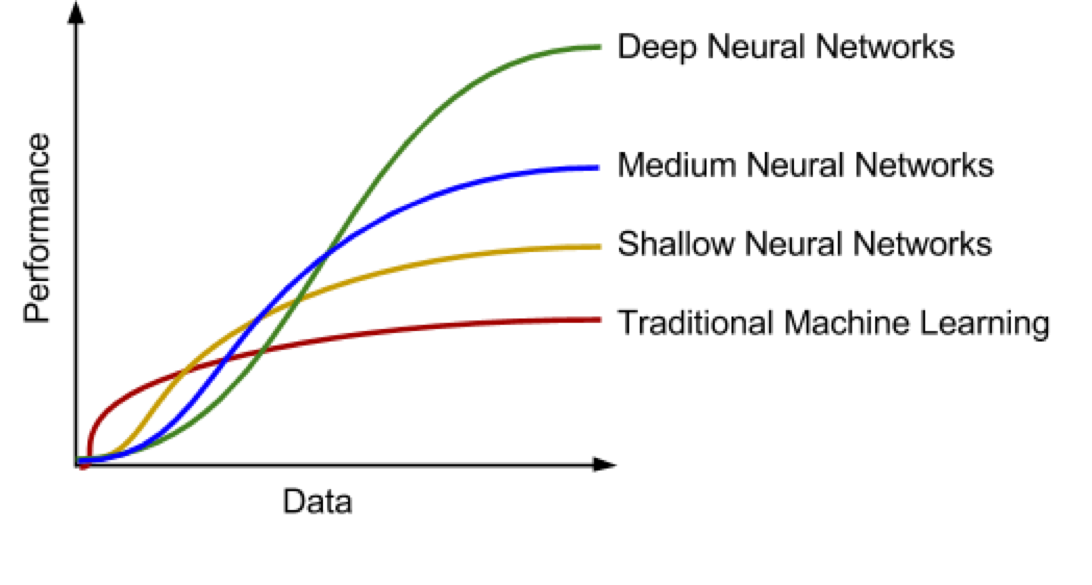
\includegraphics[scale=0.5]{images/traditionalVsDeepLearning}
\captionsetup{justification=centering}
\caption{Performance Comparison of Deep learning-based algorithms Vs Traditional Algorithms~\cite{deeplearningVstraditionalAlgorithms}.}
\label{fig:performanceCompare}
\end{figure}


%%Applications of deep learning based anomaly detection
\begin{figure}[h]
\centering
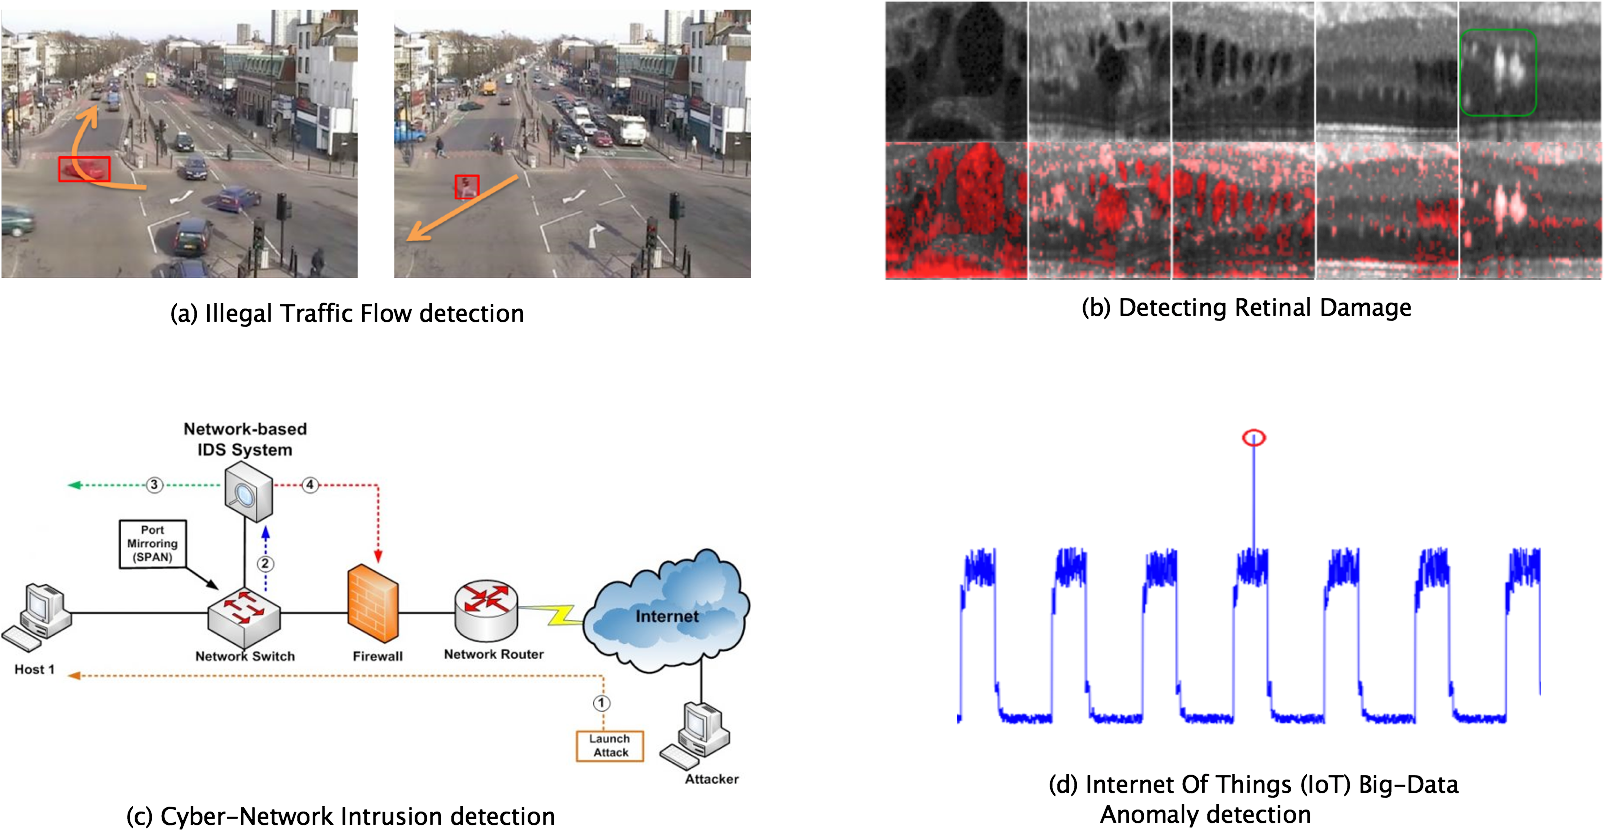
\includegraphics[scale=0.5]{images/applications}
\captionsetup{justification=centering}
\caption{Applications Deep learning-based anomaly detection algorithms.\\
(a) Video Surveillance, Image Analysis: Illegal Traffic detection~\cite{xie2017real},  (b) Health-care: Detecting Retinal Damage~\cite{schlegl2017unsupervised}\\
(c) Networks: Cyber-intrusion detection~\cite{javaid2016deep}  (d) Sensor Networks: Internet of Things (IoT) big-data anomaly detection~\cite{mohammadi2017deep} }
\label{fig:applications}
\end{figure}



%anomalies
\section{ What are anomalies ?}
Anomalies  are also referred to as abnormalities, deviants, or outliers in the data mining and statistics literature~\cite{aggarwal2013introduction}. As illustrated in Figure ~\ref{fig:anomalies}, $N_{1}$ and $N_{2}$ are regions consisting of majority of observations and hence considered as normal data instance regions, whereas the region $O_{3}$, and data points  $O_{1}$ and $O_{2}$  are few data points which are located further away from the bulk of data points and hence are considered anomalies. Anomalies may arise due to several reasons, such as malicious actions, system failures, intentional fraud, etc. These anomalies reveal interesting insights about the data and are often convey valuable information about data. Therefore, anomaly detection considered an essential step in various decision-making systems.
% Novelty Detection Definition
% \begin{figure}[h]
% 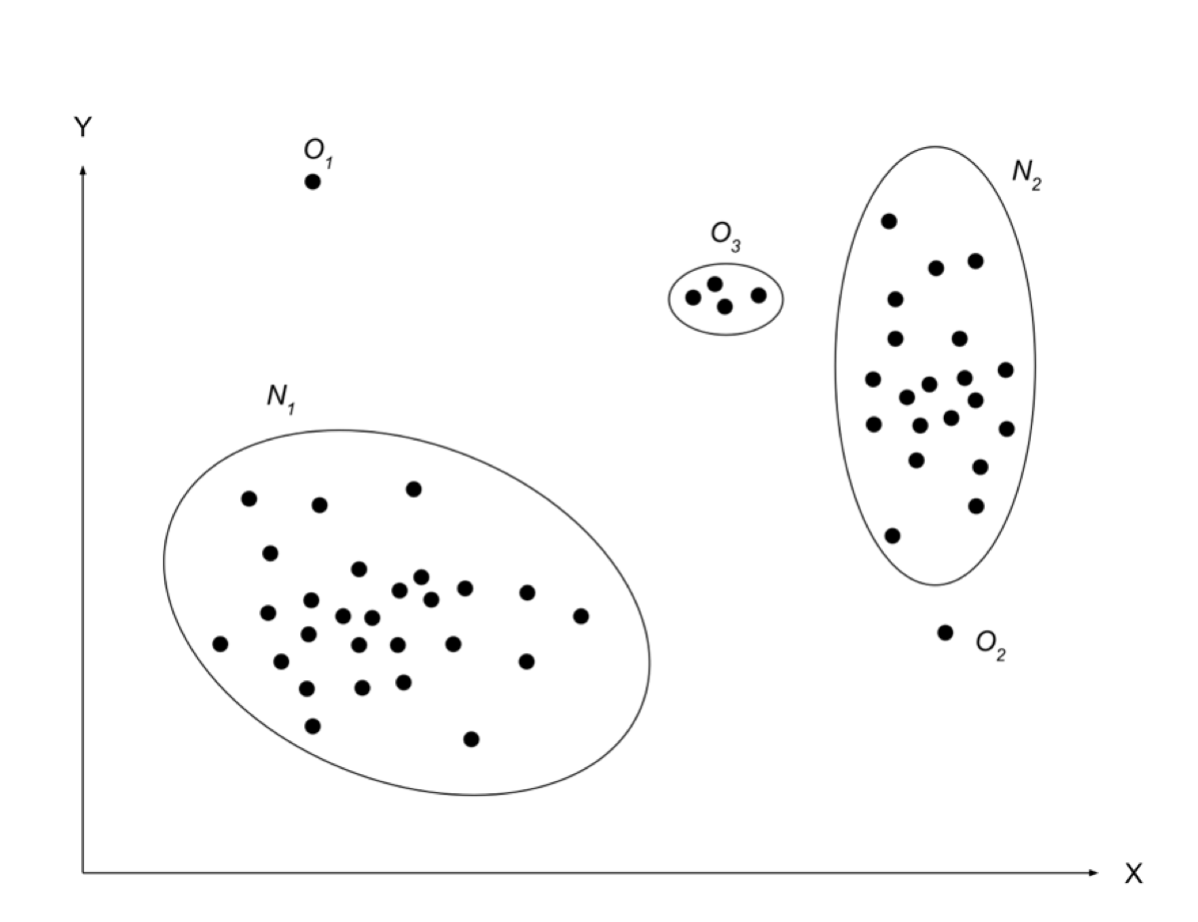
\includegraphics[scale=0.3]{images/anomalies.png}
% \caption{An illustration of anomalies in two-dimensional data set.}
% \label{fig:novelties}
% \end{figure}

% Begin of figure
\begin{figure}
  \centering
  \begin{minipage}{.48\linewidth}
    \centering
    % \subcaptionbox{}
      {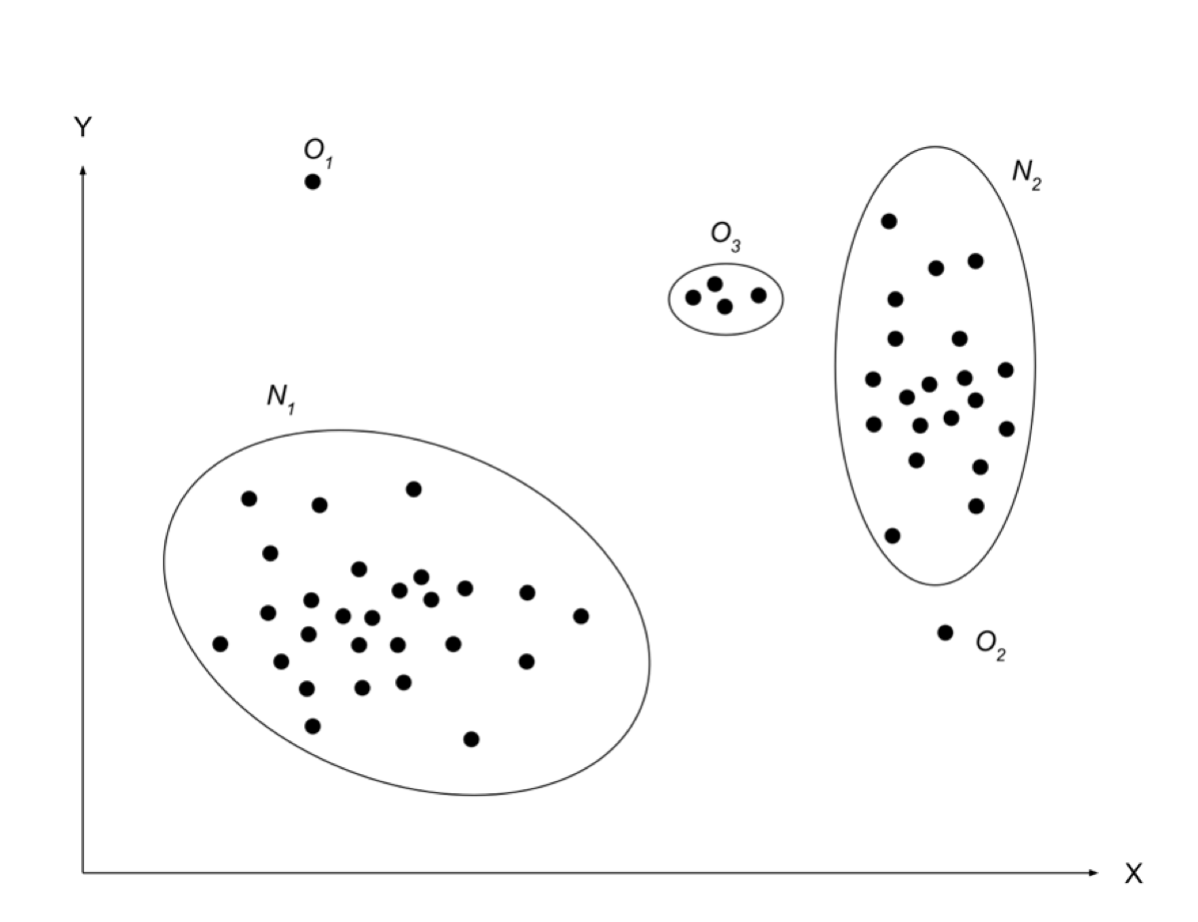
\includegraphics[scale=0.35]{images/anomalies.png}}
    \caption{Illustration of anomalies in two-dimensional data set.}
    \label{fig:anomalies}
  \end{minipage}\quad
  \begin{minipage}{.48\linewidth}
    \centering
    % \subcaptionbox{t}
      {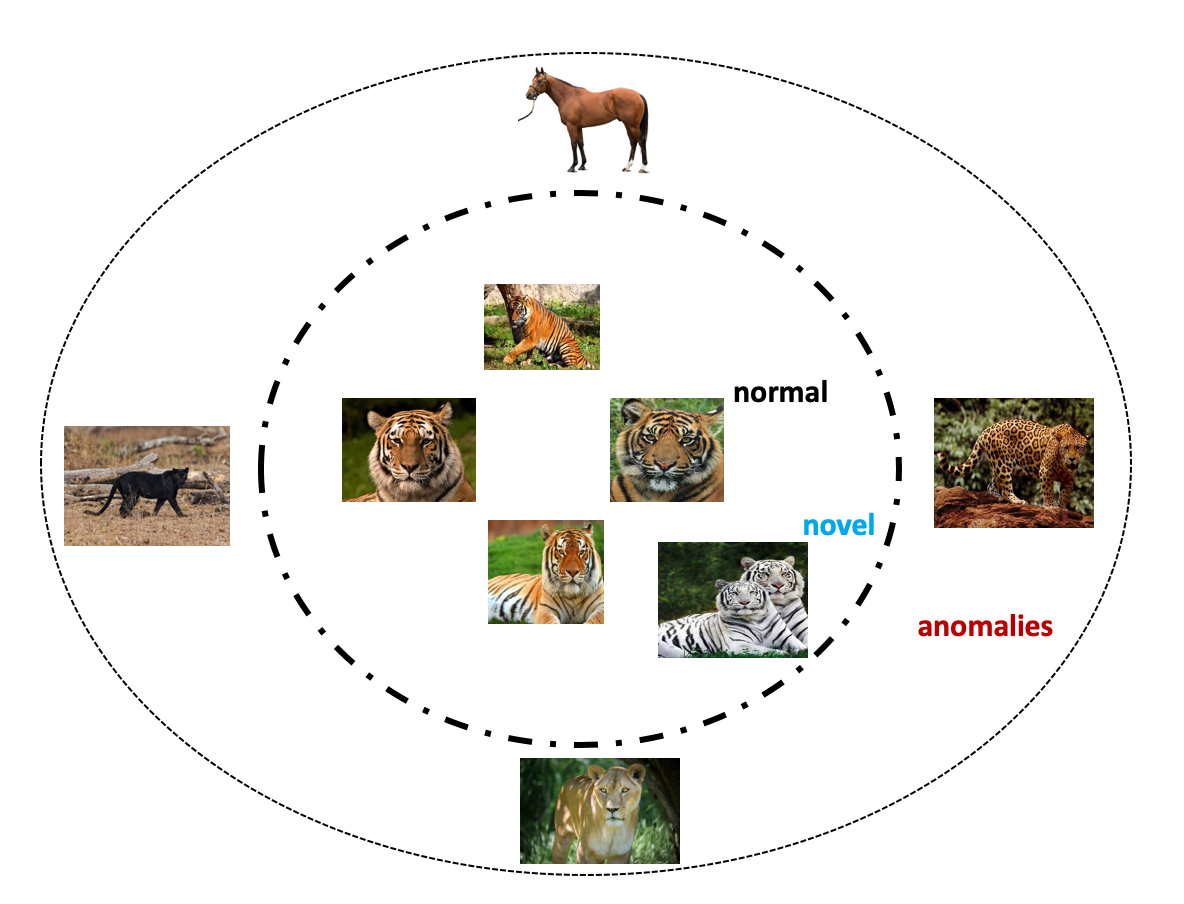
\includegraphics[scale=0.35]{images/novel.png}}
    \caption{Illustration of novelty in image data set.}
    \label{fig:novelties}
  \end{minipage}
  \bigskip

\end{figure}
% end of figure


% novelties
\section{What are novelties ?}
Novelty detection is the identification of novel (new) or unobserved patterns in the data.~\cite{miljkovic2010review}. The novelties detected are not considered as anomalous data points; instead they are incorporated into the normal data model. A novelty score may be assigned for these previously unseen data points, using a decision threshold score. ~\cite{pimentel2014review}.  The points which significantly deviate from this decision threshold may be deemed as anomalies or outliers. For instance in Figure ~\ref{fig:novelties}  the images of \textit{(white tigers)} among normal tigers may be considered as novelty, while image of \textit{(horse, panther,lion and cheetah)} are considered as anomalies.
The techniques used for anomaly detection are often used for novelty detection and vice versa.



% Challenges : Motivation and challenges Why deep learning-based anomaly detection.
\section{Motivation and Challenges: Deep anomaly detection (DAD) techniques}
\begin{itemize}
\item Performance of traditional algorithms in detecting outliers is sub-optimal on  image (e.g. medical images) and sequence data sets since it fails to capture complex structures in the data.
\item  Need for Large-scale anomaly detection : As the volume of data increases let's say to gigabytes then, it becomes nearly impossible for the traditional methods to scale to such large scale data to find outliers.
\item  Deep anomaly detection (DAD) techniques learn hierarchical discriminative features from data. This automatic feature learning capability eliminates the need of developing manual features by domain experts, therefore advocates to solve the problem end-to-end taking raw input data in domains such as text and speech recognition.
\item The boundary between normal and anomalous (erroneous) behavior is often not precisely defined  in several data domains and is constantly evolving. This lack of well defined representative normal boundary poses challenges for both conventional and deep learning-based algorithms.
\end{itemize}
% end itemize

% Begin Table
\begin{table} [ht!]
\centering
\captionsetup{justification=centering}
\caption{Comparison of our Survey to Other Related Survey Articles. \\1 \textemdash Our Survey,
2 \textemdash Kwon and Donghwoon ~\cite{kwon2017survey}, 5 \textemdash John and Derek ~\cite{ball2017comprehensive}\\
3 \textemdash Kiran  and Thomas ~\cite{kiran2018overview},            6 \textemdash Mohammadi and Al-Fuqaha ~\cite{mohammadi2017deep}\\
4 \textemdash Adewumi and Andronicus ~\cite{adewumi2017survey}       7 \textemdash Geert and  Kooi et.al ~\cite{litjens2017survey}.
}
\label{tbl:surveysummary}
\scalebox{0.75}{
\begin{tabular}{ |c|c|c|c|c|c|c|c|c|c| }
\hline
 & & 1&2&3&4&5&6&7 \\
\hline
\multirow{4}{6em}{Methods  }
&Supervised &\checkmark  & & & & & & \\
&Unsupervised &\checkmark & & & & & &  \\
&Hybrid Models & \checkmark& & & & & &  \\
&one-Class Neural Networks &\checkmark & & & & & &  \\
\hline
\multirow{8}{8em}{Applications  }
&Fraud Detection&\checkmark  & & &\checkmark & & & \\
&Cyber-Intrusion Detection&\checkmark  &\checkmark & & & & & \\
&Medical Anomaly Detection&\checkmark  & & & & & &\checkmark \\
&Sensor Networks Anomaly Detection&\checkmark  & & & &\checkmark & & \\
&Internet Of Things (IoT)
 Big-data Anomaly Detection&\checkmark  & & & & & \checkmark& \\
&Log-Anomaly Detection&\checkmark  & & & & & & \\
&Video Surveillance&\checkmark & &\checkmark  & & & & \\
&Industrial Damage Detection&\checkmark & & & & & & \\
\hline
\end{tabular}}
\end{table}
% End of Table


% Related Work
\section{Related Work}
Despite the substantial advances made by deep learning methods in many machine learning problems, there
is a relative scarcity of deep learning approaches for anomaly detection. Adewumi et.al~\cite{adewumi2017survey} provide a comprehensive survey of deep learning-based methods for fraud detection. A broad review of deep anomaly detection (DAD) techniques for cyber-intrusion detection is presented by Kwon et.al~\cite{kwon2017survey}. An extensive review of using DAD techniques in medical domain has been presented by Litjens et.al ~\cite{litjens2017survey}. An  overview of DAD techniques for Internet of Things (IoT) and  big-data anomaly detection is introduced by  Mohammadi et.al~\cite{mohammadi2017deep}. Sensor networks anomaly detection has been reviewed  by  Ball et.al~\cite{ball2017comprehensive}. The state-of-the-art deep learning based methods for video anomaly detection along with various categories has been presented in~\cite{kiran2018overview}. Although there are a number of reviews in applying DAD techniques, there is shortage of comparative analysis of deep learning architecture adopted for outlier detection. For instance a substantial amount of research on anomaly detection is conducted using deep autoencoders, but there is lack of comprehensive survey of various deep architecture's best suited for a given data-set and application domain. We hope that this survey bridges this gap and provides a comprehensive reference for researchers and engineers aspiring to leverage deep learning for anomaly detection. Table~\ref{tbl:surveysummary} shows the set of research methods and application domains covered by our survey.

% The classification taxonomy is also present in this paper $https://www.ncbi.nlm.nih.gov/pmc/articles/PMC4836738/$
% This paper~\cite{erfani2016high} presents a hybrid approach of combining deep learning models in combination with other traditional techniques to identify outliers and obtained promising results.

% Anomaly Detection Taxonomy
\begin{figure}[h]
\centering
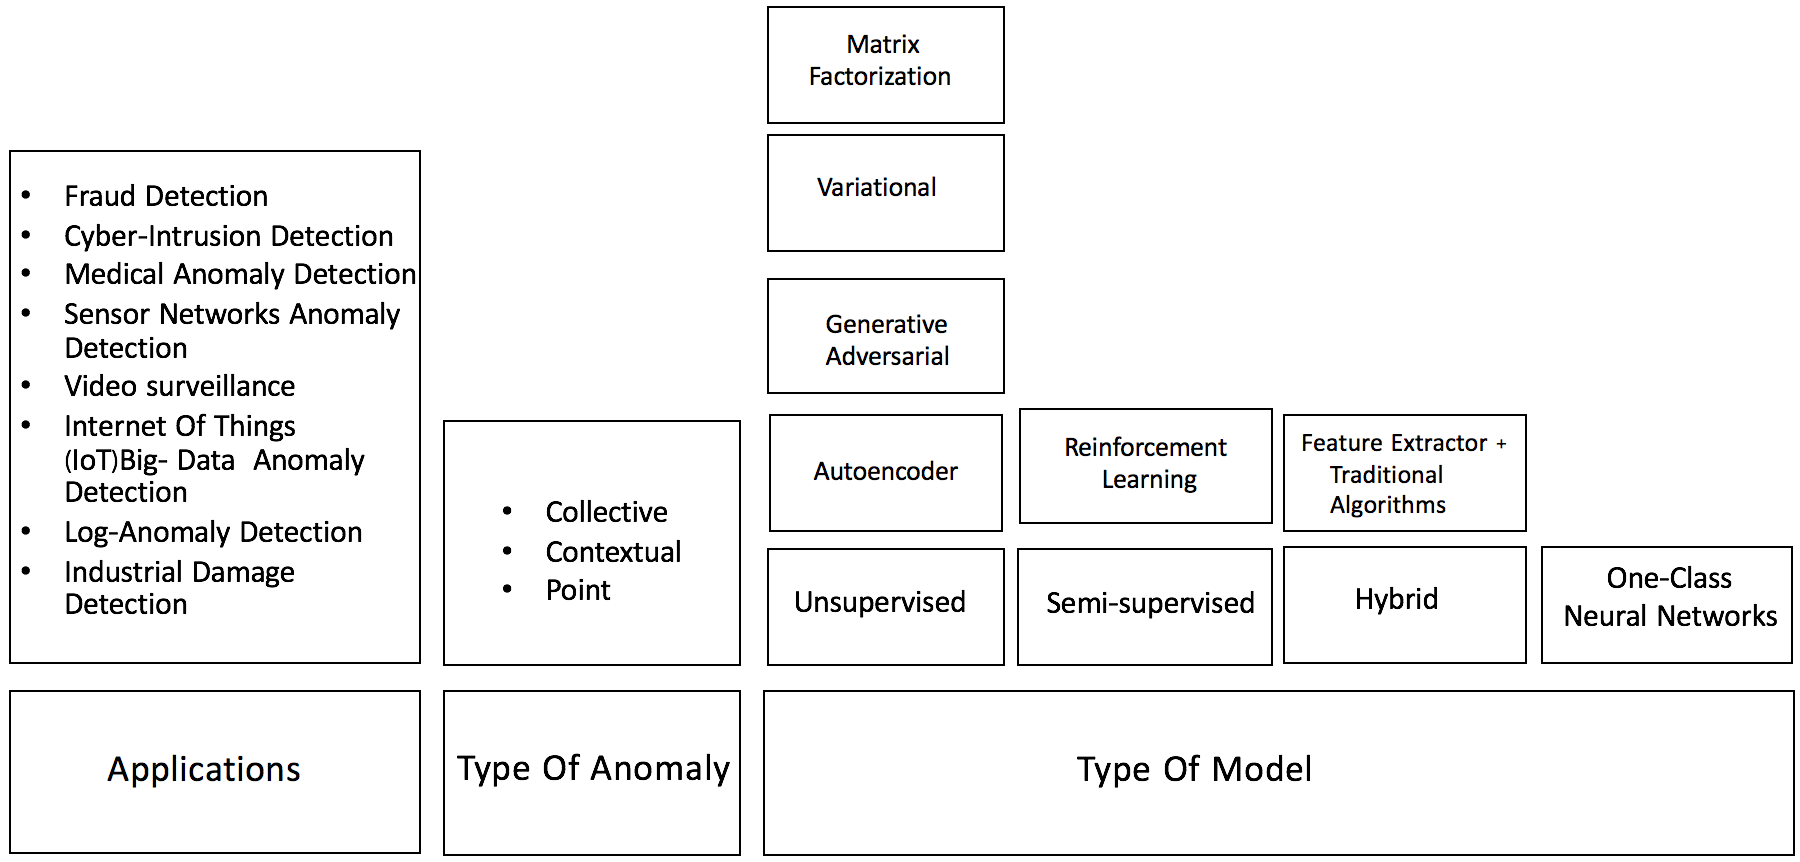
\includegraphics[scale=0.45]{images/AnomalyDetectionTaxonomy}
\caption{Key components associated with deep learning-based anomaly detection technique.}
\label{fig:surveyTaxonomy}
\end{figure}
% end of related work

%% Our Contributions
\section{ Our Contributions}
We follow survey approach of V.Chandola and A.Banerjee et.al~\cite{chandola2007outlier} for deep  anomaly detection (DAD). Our survey presents a detailed and structured overview of research and applications of DAD techniques. We summarize our main contributions as follows:
\begin{itemize}
\item Most of the existing surveys on DAD techniques either focus on a particular
application domain or specific research area of interest~\cite{kiran2018overview,mohammadi2017deep,litjens2017survey,kwon2017survey,adewumi2017survey,ball2017comprehensive}.
This review aims to provide a comprehensive outline of state-of-the art research in DAD techniques as well as several real world applications these techniques are discussed.
\item In recent years a number of new deep learning based anomaly detection techniques  with greatly reduced computational requirements have been developed. The purpose of this paper is to survey these techniques and classify them into organized schema for better understanding. We introduce two more sub-categories Hybrid models ~\cite{erfani2016high} and one-class neural networks techniques~\cite{chalapathy2018anomaly} as illustrated in Figure~\ref{fig:surveyTaxonomy} based on the choice of training objective. For each categories we discuss both the assumptions and techniques adopted for best performance. Furthermore within each category, we also present the challenges, advantages and disadvantages and provide an overview of computational complexity of DAD methods.
\end{itemize}

% Organization of the paper
\section{Organization}
This chapter is organized by following structure described in Figure~\ref{fig:surveyTaxonomy}.
In Section~\ref{sec:aspectsOfAnomalyDetection}, we identify the various aspects that determine the formulation of the problem and highlight the richness and complexity associated with anomaly detection.
We introduce and define two types of models: contextual and collective or group anomalies. In Section~\ref{sec:applicationsOfDLAD}, we briefly describe the different application domains to which deep learning-based anomaly detection has been applied. In subsequent sections we provide a categorization of deep learning-based techniques based on the research area to which they belong.  Based on training objectives employed and availability of labels  deep learning-based anomaly detection techniques  can be categorized into supervised (Section~\ref{sec:supervisedDAD}), unsupervised (Section ~\ref{sec:unsupervisedDAD}), hybrid (Section~\ref{sec:hybridModels}), and one-class neural network  (Section~\ref{sec:oneclassNN}). For each category of techniques we also discuss their computational complexity for training and testing phases. In Section~\ref{sec:typeBasedAD} we discuss  point, contextual, and collective (group) deep learning-based anomaly detection techniques. We present some discussion of the limitations and relative performance of various existing techniques in Section~\ref{sec:relativeSOW}. Section~\ref{sec:chapter1_conclusion} contains concluding remarks.

% \titlespacing{\section}{0pt}{2ex}{1ex}

\section{Different aspects of deep learning-based anomaly detection. }
\label{sec:aspectsOfAnomalyDetection}
This section identifies and discusses the different aspects of deep learning-based anomaly detection.

%%%%%%%%%%%%%%%%%%%%%%%% Begin of  Nature of Input data %%%%%%%%%%%%%%%%%%%%%%%%
\subsection{ Nature of Input Data}
The choice of deep neural network architecture in deep anomaly detection methods primarily depends on the nature of input data. Input data can be broadly classified into sequential (eg, voice, text, music, time series, protein sequences) or non-sequential data (eg, images, other data). Table~\ref{tab:dataTypeModelArchitecture} illustrates the nature of input data and deep model architectures used in anomaly detection. Additionally input data depending on the number of features (or attributes) can be further classified into either low or high-dimensional data. DAD techniques have been to learn complex hierarchical feature relations within high-dimensional raw input data ~\cite{lecun2015deep}. The number of layers used in DAD techniques is driven by input data dimension, deeper networks are shown to produce better performance on high dimensional data. Later on in the Section ~\ref{sec:deepDADModels}  various models considered for outlier detection are reviewed at depth.

%% Create a table with Type of data and kind of architecture suitable for anomaly detection.
% %%%%%%%%%%%%%%%%%%%%%%%% End of  Nature of Input data %%%%%%%%%%%%%%%%%%%%%%%%
%%%%%%%%%%%%%%%%%%%%%%%% Begin  Type of models %%%%%%%%%%%%%%%%%%%%%%%%
\subsection{Based on Availability of labels}
Labels indicate whether a chosen data instance is normal or outlier. Anomalies are rare entities hence it is very  difficult to obtain their labels. Furthermore anomalous behaviour may change over time, for instance  the nature of anomaly had changed so significantly and that it  remained unnoticed at Maroochy water treatment plant, for a long time which resulted in leakage of 150 million litres of untreated sewerage to local waterways ~\cite{ramotsoela2018survey}.\\
Deep anomaly detection (DAD) models can be categorized into three categories based on extent of availability of labels. (1) Supervised deep anomaly detection. (2) Semi-supervised deep anomaly detection. (3) Unsupervised deep anomaly detection.

\subsubsection{Supervised deep anomaly detection}
\label{supervised_learning}
Supervised deep anomaly detection involves training a deep supervised binary or multi-class classifier, using labels of both normal and anomalous data instances. For instance supervised DAD models, formulated as multi-class classifier aids in detecting rare brands, prohibited drug name mention and fraudulent health-care transactions~\cite{chalapathy2016investigation,chalapathy2016bidirectional}.
Despite the improved performance of supervised DAD methods, these methods are not as popular as semi-supervised or unsupervised methods, owing to lack of availability of labeled training samples. Moreover the performance of deep supervised classifier used as anomaly detector is sub-optimal due to class imbalance (the total number of positive class instances are far more than the total number of (negative) class of data). Therefore we do not consider the review of supervised DAD methods in this survey.

\begin{table}
\centering
\scalebox{0.99}{
\begin{tabular}{ |c|c|c|c| }
\hline
Type of Data & Examples & DAD model architecture  \\ [0.5ex]
\hline
\multirow{3}{3em}{Sequential} & Video,Speech &  \\
&Protein Sequence,Time Series  & CNN, RNN, LSTM  \\
&Text (Natural language)  &  \\
\hline
\multirow{2}{3em}{Non-Sequential} & Image,Sensor &  \\
&Other (data)  & CNN, AE and its variants  \\
\hline
\end{tabular}}
\caption{Table illustrating nature of input data and corresponding deep anomaly detection model architectures proposed in literature.
        \\CNN: Convolution Neural Networks, LSTM : Long Short Term Memory Networks \\
         AE: Autoencoders. }
\label{tab:dataTypeModelArchitecture}
\end{table}
% End of table
\subsubsection{Semi-supervised deep anomaly detection}
\label{semi_supervised_learning}
The labels of normal instances are far more easy to obtain than anomalies, as a result semi-supervised DAD techniques are more widely adopted, these techniques leverage existing labels of single (normally positive class) to separate outliers. One common way of using deep autoencoders  in anomaly detection is to train them in a semi-supervised way on data samples with no anomalies. With sufficient training samples, of normal class autoencoders would produce low reconstruction errors for normal instances, over anomalous events.
~\cite{wulsin2010semi,nadeem2016semi,song2017hybrid}. We consider detailed review of these methods in  Section~\ref{sec:semi_supervised_DAD}.

%% Taxonomy of Models
%performance comparision
\begin{figure}[h]
\centering
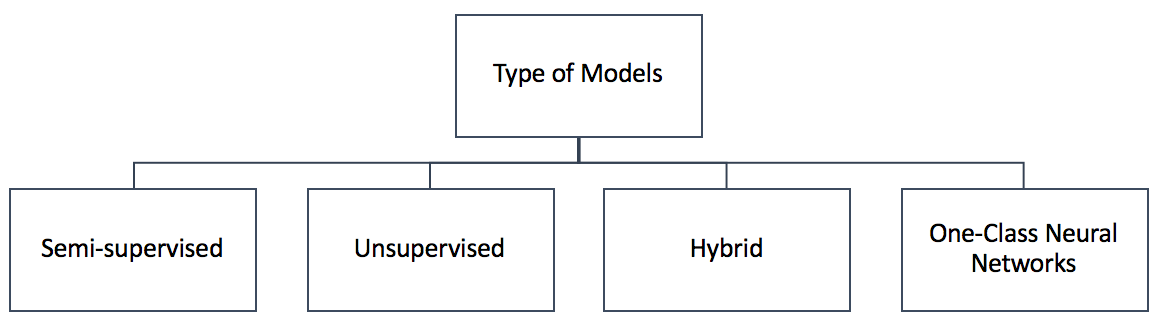
\includegraphics[scale=0.7]{images/TypeOfModels}
\captionsetup{justification=centering}
\caption{Taxonomy based on type of deep learning models for anomaly detection.}
\label{fig:typeOfModels}
\end{figure}

\subsubsection{Unsupervised deep anomaly detection}
\label{sec:USAD}

Unsupervised deep anomaly detection techniques detect outliers solely based on intrinsic properties of the data instances. Unsupervised DAD techniques are used in automatic labelling of unlabelled data samples since labeled data is very hard to obtain ~\cite{patterson2017deep}. Variants of Unsupervised DAD models~\cite{tuor2017deep} are shown to outperform traditional methods such as principal component analysis (PCA) ~\cite{wold1987principal}, support vector machine (SVM) ~\cite{cortes1995support} and Isolation Forest~\cite{liu2008isolation} techniques in applications domains such as health and cyber security.
Autoencoders are the core of all Unsupervised DAD models. These models assume the high prevalence of normal instances than abnormal data instances failing which would result in high false positive rate. Additionally unsupervised learning algorithms such as restricted Boltzmann machine (RBM)~\cite{sutskever2009recurrent}, deep Boltzmann machine (DBM), deep belief network (DBN)~\cite{salakhutdinov2010efficient}, generalized denoising autoencoders~\cite{vincent2008extracting} , recurrent neural network (RNN)~\cite{rodriguez1999recurrent} Long short term memory networks~\cite{lample2016neural} which are used to detect outliers are discussed in detail in Section ~\ref{sec:rnn_lstm_gru}.

\subsection{Based on training objective}
In this survey we introduce two new categories of deep anomaly detection (DAD) techniques based on training objective employed 1) Deep hybrid models (DHM). 2) One class neural networks (OC-NN).

\subsubsection{Deep Hybrid Models (DHM)}
\label{sec:DHM}

Deep hybrid models for anomaly detection use deep neural networks mainly autoencoders as feature extractors, the features learned within the hidden representations of autoencoders are input to traditional anomaly detection algorithms such as one-class SVM (OC-SVM) to detect outliers~\cite{andrews2016detecting}. Figure~\ref{fig:HybridDeepModels} illustrates  the deep hybrid model architecture used for anomaly detection. Following the success of transfer learning to obtain rich representative features  from models pre-trained on large data-sets,  hybrid models have also employed these pre-trained transfer learning models as feature extractors with great success ~\cite{pan2010survey}. A variant of hybrid model was proposed by  Ergen et.al~\cite{ergen2017unsupervised} which considers joint training of feature extractor along-with OC-SVM (or SVDD) objective to maximize the detection performance. A notable shortcoming of these hybrid approaches
is the lack of trainable objective customized for anomaly detection, hence these models fail to extract rich differential features to detect outliers.  In order to overcome this limitation customized objective for anomaly detection such Deep one-class classification~\cite{ruff2018deep}and  One class neural networks~\cite{chalapathy2018anomaly} are introduced.

\begin{figure*}
\centering
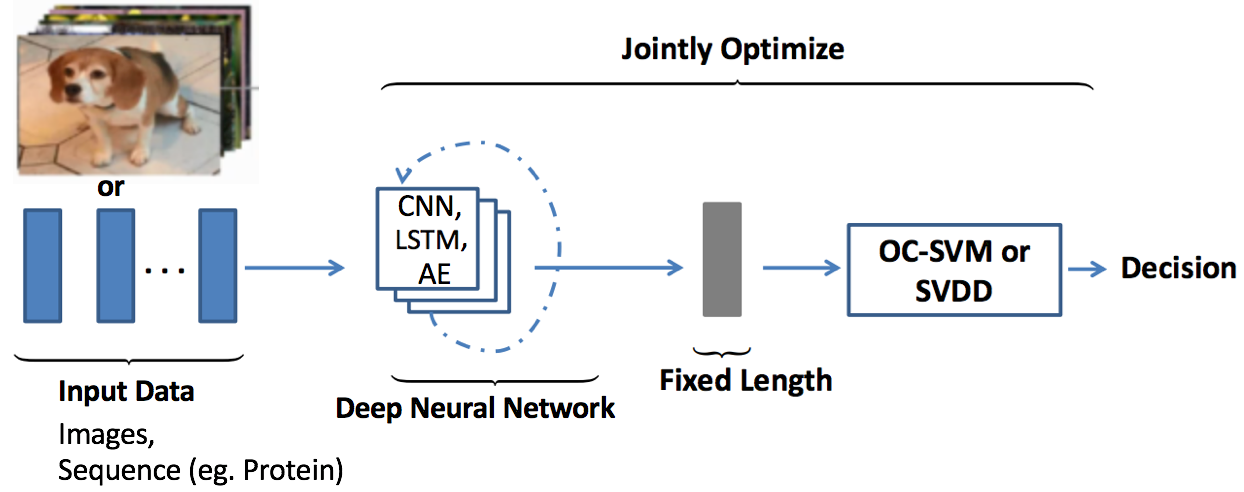
\includegraphics[scale=0.7]{images/HybridDeepModels}
\captionsetup{justification=centering}
\caption{Deep Hybrid Model Architecture.}
\label{fig:HybridDeepModels}
\end{figure*}


\subsubsection{One-Class Neural Networks (OC-NN)}
\label{sec:oc-nn}

One class neural network (OC-NN)~\cite{chalapathy2018anomaly} methods are inspired by kernel-based one-class classification which combines the ability of deep networks to extract progressively rich representation of data with the one-class objective of creating a tight envelope around normal data. The OC-NN approach breaks new ground for the following crucial reason: data representation in the hidden layer is driven by the OC-NN objective and is thus customized for anomaly detection. This is a departure from other approaches which use a hybrid approach of learning deep features using an autoencoder and then feeding the features into a separate anomaly detection method like one-class SVM (OC-SVM).  The details of training and evaluation of one class neural networks is discussed in Chapter ~\ref{chpt:ocnn} . Another variant of one class neural network architecture Deep Support Vector Data Description (Deep SVDD)~\cite{ruff2018deep} trains deep neural network to extract common factors of variation by closely mapping the normal data instances to the center of sphere, is shown to produce performance improvements on MNIST~\cite{lecun2010mnist} and CIFAR-10 ~\cite{krizhevsky2009learning} datasets.


%%%%%%%%%%%%%%%%%%%%%%%% End  Type of Models %%%%%%%%%%%%%%%%%%%%%%%%


\subsection{Type of Anomaly}
\label{sec:typeBasedAD}
Anomalies can be broadly  classified into three types: point anomalies, contextual anomalies and collective anomalies. Deep anomaly detection (DAD) methods have been shown to detect all three types of anomalies with great success.

% classification tree
\begin{figure}[h]
\centering
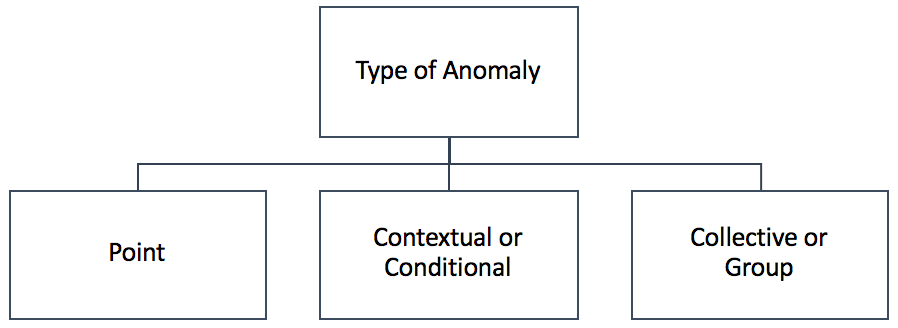
\includegraphics[scale=0.7]{images/TypeOfAnomaly}
\captionsetup{justification=centering}
\caption{Deep learning techniques classification based on type of anomaly.}
\label{fig:typeOfAnomaly}
\end{figure}


% Point Anomaly
\subsubsection{Point Anomalies.}
The majority of work in literature focuses on point anomalies. Point anomalies often represent an irregularity or deviation that happens randomly and may have no particular interpretation. For instance in Figure~\ref{fig:PointAndCollectiveAnomaly} a credit card transaction with high expenditure recorded at
\textit{Monaco} restaurant seems a point anomaly since it significantly deviates from the rest of the transactions. Several real world applications, considering point anomaly detection are reviewed in Section~\ref{sec:applicationsOfDLAD}.

% Contextual Anomaly
\subsubsection{Contextual Anomaly Detection}
\label{sec:contextualanomalies}
Contextual anomaly also referred as conditional anomaly is a data instance that could be considered as anomalous in some specific context~\cite{song2007conditional}. The contextual anomaly is identified by considering both contextual and behavioural features.
The contextual features, normally used are time and space. While the behavioral features may be pattern of spending money, occurence of system log events, or any feature used to describe the normal behaviour.
Figure ~\ref{fig:2dtemp} illustrates the example of contextual anomaly considering temperature data indicated by a drastic drop just before June, this value is not indicative of a normal value found during this time. Figure ~\ref{fig:syslog} illustrates using deep Long Short-Term Memory (LSTM)~\cite{hochreiter1997long}  based model to identify anomalous system log events ~\cite{du2017deeplog} in a given context (e.g event 53 is detected as being out of context).

% % Begin of figure
% \begin{figure}
%   \centering
%   \begin{minipage}{.48\linewidth}
%     \centering
%     % \subcaptionbox{}
%       {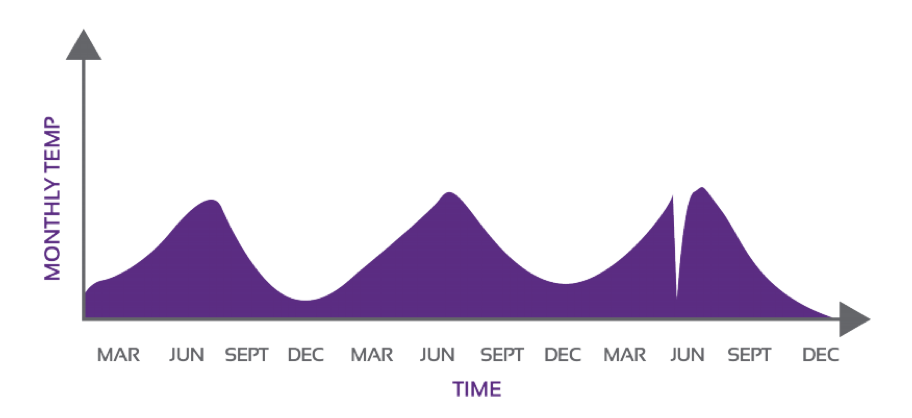
\includegraphics[scale=0.35]{images/temperature.png}}
%     \caption{Anomaly within two-dimensional temperature data set.}
%     \label{fig:temperatureContextual}
%   \end{minipage}\quad
%   \begin{minipage}{.48\linewidth}
%     \centering
%     % \subcaptionbox{t}
%       {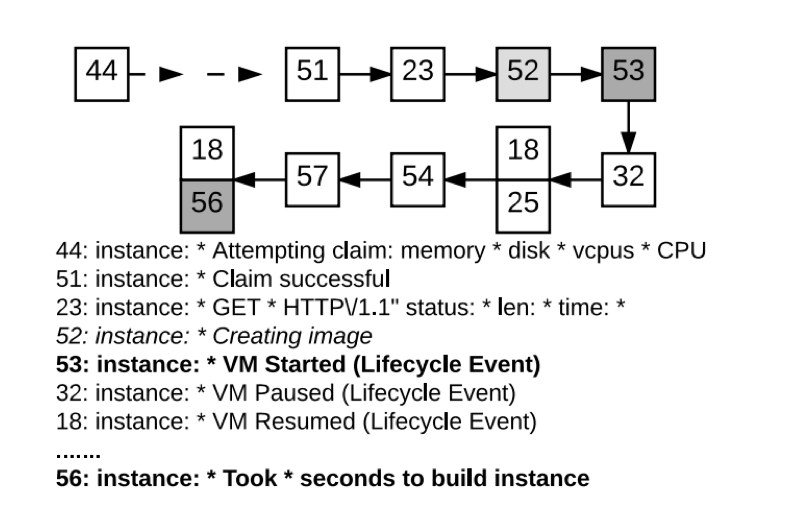
\includegraphics[scale=0.35]{images/deeplog.png}}
%     \caption{Anomaly within system logs.}
%     \label{fig:deeplogContextual}
%   \end{minipage}
%   \bigskip
% \end{figure}
% % end of figure


% Begin figure
\begin{figure}[htp]
  % Fixed length
  \centering
  \subcaptionbox{ Temperature data~\cite{hayes2015contextual}.\label{fig:2dtemp}}{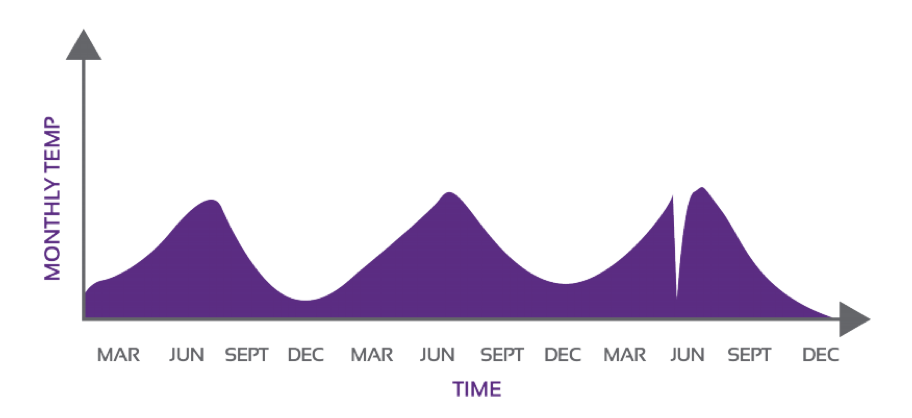
\includegraphics[scale=0.35]{images/temperature.png}}\hspace{1em}%
  \subcaptionbox{System logs ~\cite{du2017deeplog}.\label{fig:syslog}}{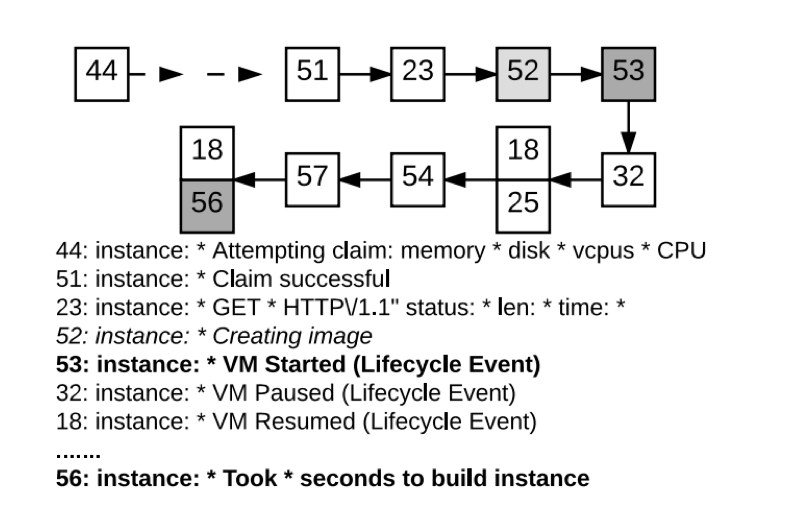
\includegraphics[scale=0.35]{images/deeplog.png}}
  \caption{Illustration of contextual anomaly detection.}
        \label{fig:deeplogContextual}
\end{figure}
% End of figure



% classification tree
% \begin{figure}[h]
% 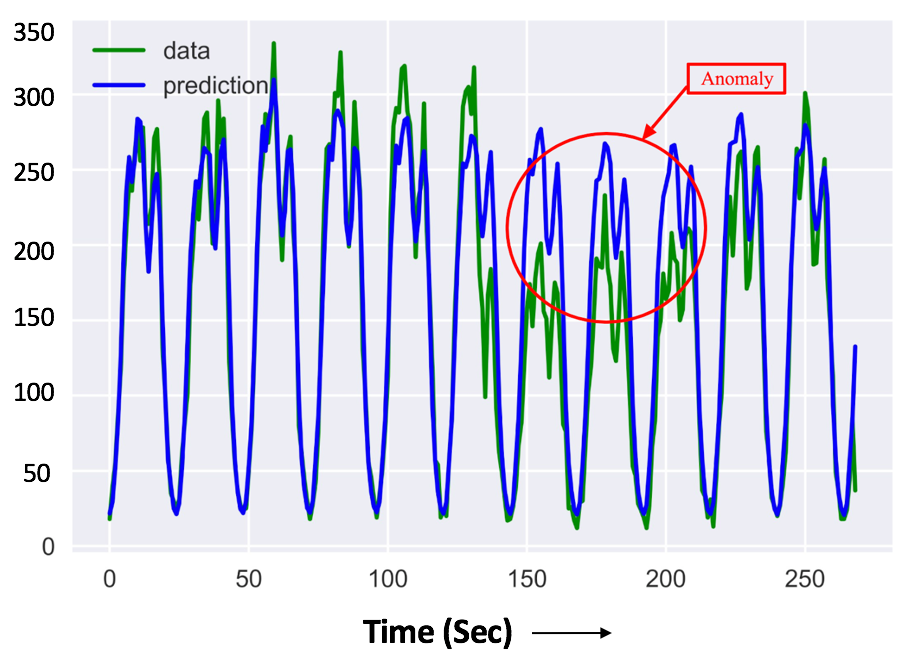
\includegraphics[scale=0.5]{images/ContextualAnomaly}
% \captionsetup{justification=centering}
% \caption{Predicted Vs Actual Data : Illustrating Contextual Anomaly.}
% \label{fig:ContextualAnomaly}
% \end{figure}


% Collective or Group Anomaly detection
\subsubsection{Collective or Group Anomaly Detection.}
Anomalous collections of individual data points are known as collective or group anomalies, wherein each of the individual points in isolation appear as normal data instances while observed in a group exhibit unusual characteristics. For example, consider an illustration of fraudulent credit card transaction, in the log data shown in Figure~\ref{fig:PointAndCollectiveAnomaly}, if a single transaction of "MISC" would have occured, it might probably not seem as anomalous. The consecutive group of transactions of valued at $\$75$ certainly seems to be a candidate for collective or group anomaly.
Group anomaly detection (GAD) with an emphasis on irregular group distributions (e.g. irregular mixtures of image pixels are detected using a variant of autoencoder model~\cite{chalapathy2018group,bontemps2016collective,araya2016collective,zhuang2017group}
% classification tree
\begin{figure}[h]
\centering
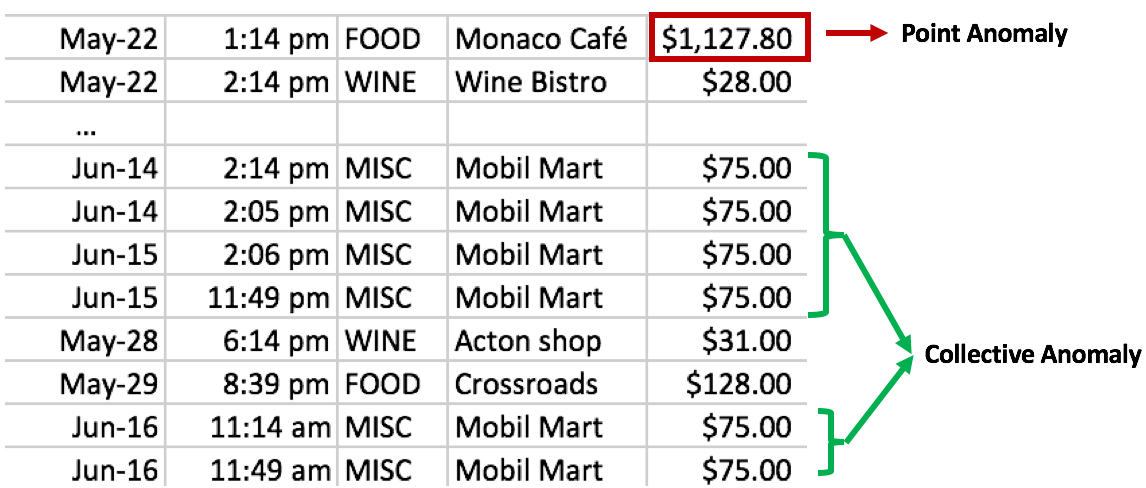
\includegraphics[scale=0.5]{images/PointAndCollectiveAnomaly}
\captionsetup{justification=centering}
\caption{Credit Card Fraud Detection: Illustrating Point and Collective anomaly.}
\label{fig:PointAndCollectiveAnomaly}
\end{figure}
%%%%%%%%%%%%%%%%%%%%%%%% End  Type of Anomalies %%%%%%%%%%%%%%%%%%%%%%%%


% Collective anomaly is also known as  group anomaly. While each individual data instances of this group may not be an anomaly, but their occurrence together as a collection is anomalous.

% Output of deep learning based anomaly detection methods
\subsection {Output of DAD Techniques}
\label{output_of_dad_methods}
An critical aspect for anomaly detection methods is the way in which the anomalies are identified. Generally, the outputs produced by anomaly detection methods are either anomaly score or binary labels.

\subsubsection{Anomaly Score:}
 Anomaly score describes the level of \textit{outlierness} for  each datapoint. The data instances may be ranked according to  anomalous score, and a domain specific threshold (commonly known as decision score) will be selected by subject matter expert to identify the anomalies.  In general, decision scores reveal more information than binary labels. For instance in Deep SVDD approach the decision score is the measure of distance of data point from center of the sphere, the data points which are farther away from center are considered anomalous~\cite{pmlrv80ruff18a}.

\subsubsection{Labels:} Instead of assigning scores, some techniques may assign a category label as normal or anomalous to each data instance. Unsupervised anomaly detection techniques using autoencoders measure  the magnitude of residual vector (i,e reconstruction error) for obtaining anomaly scores, later on the reconstruction errors are either ranked or thresholded by domain experts to label data instances.
%%%%%%%%%%%%%%%%%%%%%%%% End  Output of deep learning based AD %%%%%%%%%%%%%%%%%%%%%%%%


%!TEX root = ../main.tex
\section{Applications of Deep Anomaly Detection}
\label{sec:applicationsOfDLAD}

In this section we discuss several applications of deep anomaly detection. For each application
domain we discuss the following four aspects:\\
\textemdash the notion of anomaly;\\
\textemdash nature of the data;\\
\textemdash challenges associated with detecting anomalies;\\
\textemdash existing deep anomaly detection techniques.\\

%!TEX root = ../../main.tex
\subsection{Intrusion Detection}
\label{sec:intrusion_detection}

Intrusion detection  system (IDS) refers to identifying malicious activity in a computer related system~\cite{phoha2002internet}. IDS may be deployed at single computers known as Host Intrusion Detection (HIDS) to large networks Network Intrusion Detection (NIDS). The classification of deep anomaly detection techniques for intrusion detection is in Figure ~\ref{fig:deepADforIDS}. IDS depending on detection method are classified into signature based or anomaly based. Using signature based IDS is not efficient to detect new attacks, for which no specific signature pattern is available, hence anomaly based detection methods are more popular. In this survey we focus on deep anomaly detection (DAD) methods and architectures employed in intrusion detection.
\vspace{-0.3cm}
\subsubsection{Host-Based Intrusion Detection Systems (HIDS):}
 Such systems are installed software programs which monitors a single host or computer for malicious  activity or policy violations by listening to system calls or events occurring within that host ~\cite{vigna2005host}. The system call logs could be generated by programs or by user interaction resulting in logs as shown in Figure ~\ref{fig:syslog}. Malicious interactions lead to execution of these system calls in different sequences. HIDS may also monitor the state of a system, its stored information, in Random Access Memory (RAM), in the file system, log files or elsewhere for a valid sequence.
 Deep anomaly detection (DAD) techniques applied for HIDS are required to handle the variable length and sequential nature of data. The DAD techniques have to either model the sequence data or compute similarity between sequences. Some of the success-full DAD techniques for HIDS is illustrated in Table~\ref{tab:HIDS}.

\subsubsection{Network Intrusion Detection Systems (NIDS):} NIDS systems deal with monitoring the entire network for suspicious traffic by examining each and every network packet. Owing to real-time streaming behaviour, the nature of data is synonymous to big data with high volume, velocity, variety. The network data also has a temporal aspect associated with it. Some of the success-full DAD techniques for NIDS is illustrated in Table~\ref{tab:NIDS}. This survey also lists the data-sets used for evaluating the DAD intrusion detection methods in Table~\ref{tab:IDSDataset}. A challenge faced by DAD techniques in intrusion detection is that the nature of anomalies keeps changing over time as the intruders adapt their network attacks to evade the existing intrusion detection solutions.

% Begin Figure
\begin{figure*}
\centering
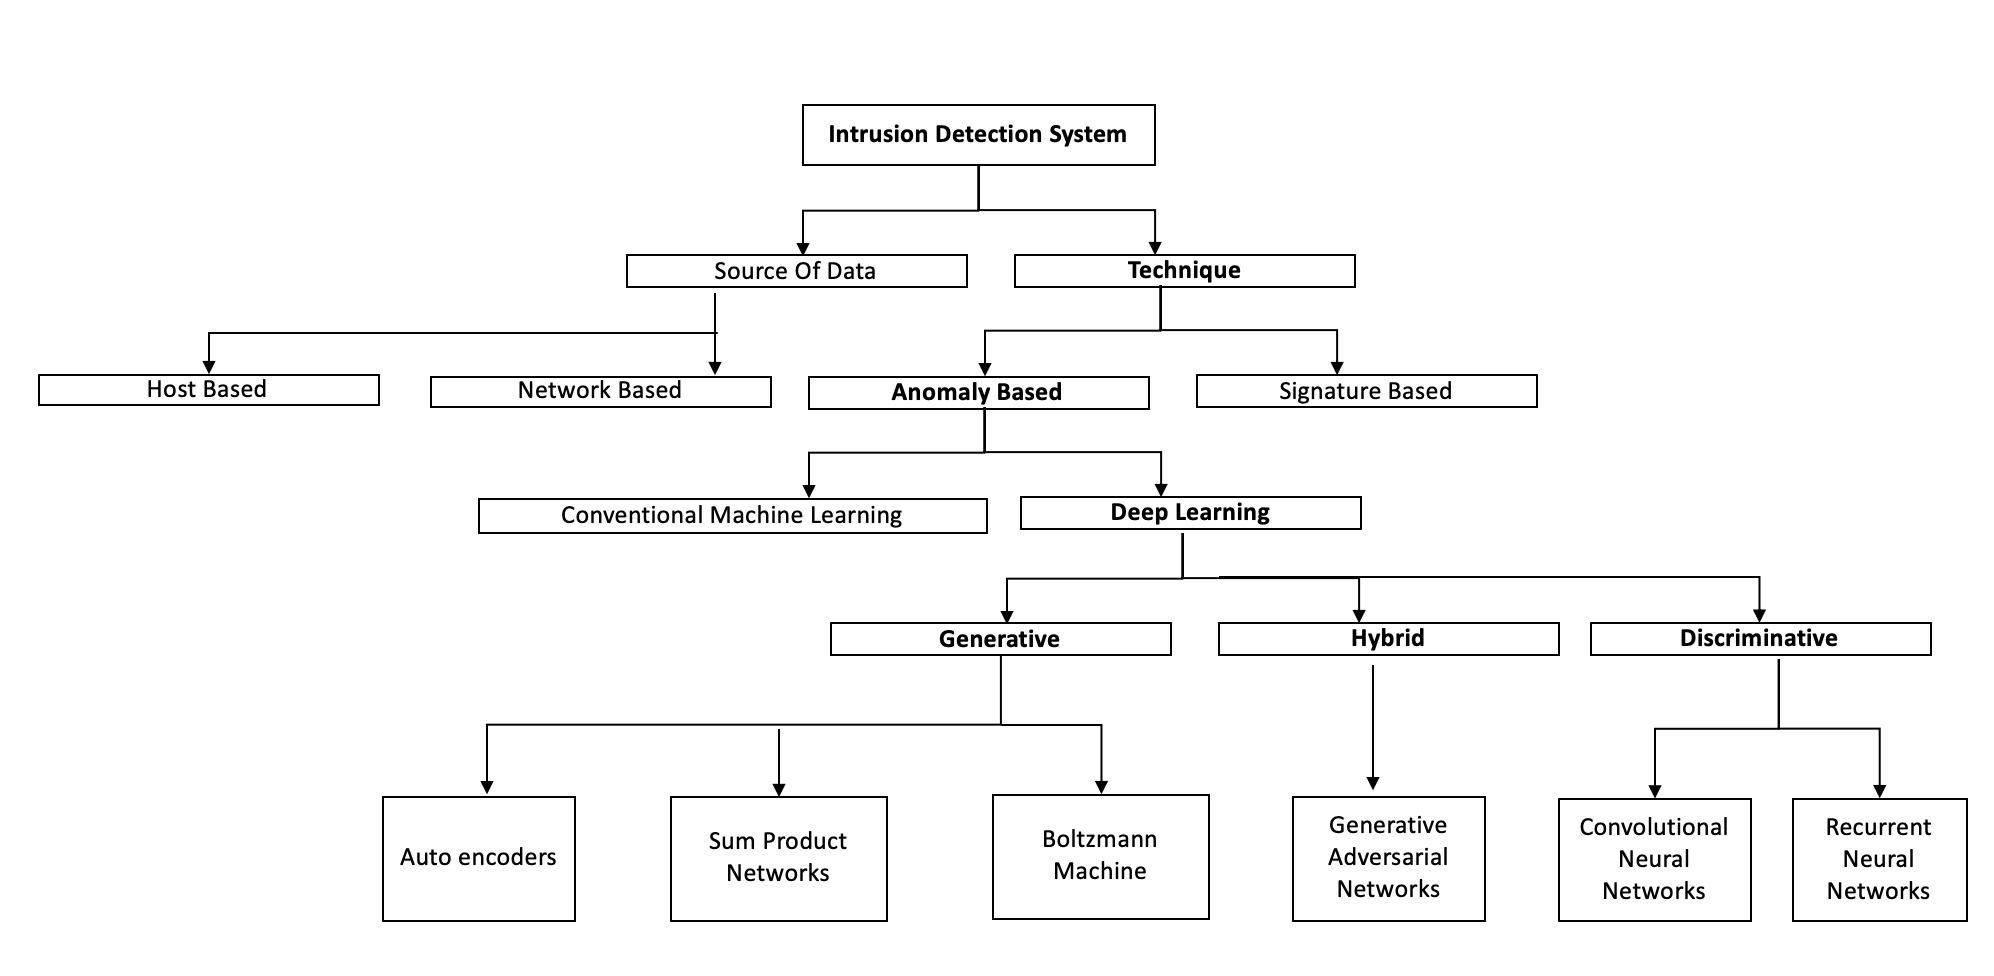
\includegraphics[scale=0.4]{images/IDS}
\captionsetup{justification=centering}
\caption{Classification of deep learning methods for intrusion detection.}
\label{fig:deepADforIDS}
\end{figure*}
% End of Figure


%%%%%%% HIDS Network intrusion detection%%%%%%%
%%% Table  Describing the model architectures and techniques used  of HIDS
\begin{table}
\begin{center}
\caption{Examples of DAD Techniques employed in HIDS
          \\CNN: Convolution Neural Networks, LSTM : Long Short Term Memory Networks
          \\GRU: Gated Recurrent Unit, DNN : Deep Neural Networks
          \\SPN: Sum Product Networks}
 \captionsetup{justification=centering}
  \label{tab:HIDS}
   \scalebox{0.82}{
    \begin{tabular}{ | l | p{4cm} | l | p{5cm} |}
    \hline
    Techniques & Model Architecture & Section & References \\ \hline
    Discriminative &  LSTM , CNN-LSTM-GRU, DNN & Section ~\ref{sec:rnn_lstm_gru},~\ref{sec:cnn},~\ref{sec:dnn} &  \cite{kim2016lstm},\cite{chawla2018host},\cite{chen2018henet},\cite{sohi2018recurrent},\cite{vinayakumar2017applying} \\\hline
    Hybrid &  GAN & Section ~\ref{sec:hybridModels} & \cite{aghakhani2018detecting}, \cite{li2018anomaly} \\\hline
    Generative &  AE, SPN,  & Section ~\ref{sec:ae},~\ref{sec:spn} & \cite{gao2014intrusion},\cite{peharz2018probabilistic},\cite{umer2018two} \\
    \hline
    \end{tabular}}
\end{center}
\end{table}
%%%% End of Table NIDS




%%% Host based Intrusion detection system table%%%%%%
%%% Table  Describing the model architectures and techniques used  of NIDS
\begin{table}
\begin{center}
  \caption{Examples of DAD Techniques employed in NIDS.
          \\CNN: Convolution Neural Networks, LSTM : Long Short Term Memory Networks
          \\RNN: Recurrent Neural Networks, RBM : Restricted Boltzmann Machines
          \\DCA: Dilated Convolution Autoencoders, DBN : Deep Belief Network
          \\AE: Autoencoders, SAE: Stacked Autoencoders
          \\GAN: Generative Adversarial Networks, CVAE : Convolutional Variational Autoencoder. }
  \captionsetup{justification=centering}

  \label{tab:NIDS}
  \scalebox{0.80}{
    \begin{tabular}{ | l | p{4cm} | p{5cm}  | p{7cm} |}
    \hline
    Techniques & Model Architecture & Section & References \\ \hline
   Generative  & DCA, SAE, RBM, DBN, CVAE & Section ~\ref{sec:cnn},~\ref{sec:ae},~\ref{sec:dnn},~\ref{sec:gan_adversarial} & \cite{yu2017network},\cite{thing2017ieee}, \cite{zolotukhin2016increasing},~\cite{cordero2016analyzing},\cite{alrawashdeh2016toward},\cite{tang2016deep},\cite{lopez2017conditional},\cite{al2018deep},\cite{mirsky2018kitsune},\cite{aygun2017network} \\ \hline
  Hybrid  & GAN   & Section ~\ref{sec:hybridModels} & \cite{lin2018idsgan},\cite{yin2018enhancing}, \cite{ring2018flow}, \cite{latah2018deep},\cite{intrator2018mdgan},\cite{matsubara2018anomaly},~\cite{nicolau2016hybrid} ,\cite{rigaki2017adversarial}. \\ \hline
  Discriminative &  RNN , LSTM ,CNN & Section ~\ref{sec:rnn_lstm_gru},~\ref{sec:cnn} & \cite{yu2017network}, \cite{malaiya2018empirical} \cite{kwon2018empirical},\cite{gao2014intrusion},\cite{staudemeyer2015applying},\cite{naseer2018enhanced}\\
  \hline
  \end{tabular}}
\end{center}
\end{table}
%%%% End of Table NIDS


% Datasets Used Table
%%% Host based Intrusion detection system table%%%%%%
%%% Table  Describing the model architectures and techniques used  of NIDS
\begin{table*}
\begin{center}
  \caption{Datasets Used in Intrusion Detection }
   \label{tab:IDSDataset}
    \scalebox{0.85}{
    \begin{tabular}{ | p{3cm} | l | p{5cm} | p{3cm} | p{5cm} |}
    \hline
    DataSet &IDS & Description & Type & References \\ \hline
    CTU-UNB & NIDS & CTU-UNB~\cite{ucsdAnomalyDetect2017} dataset consists of various botnet traffics from CTU-13 dataset [20] and normal traffics from the UNB ISCX IDS 2012 dataset ~\cite{shiravi2012toward}  & Hexadecimal & \cite{yu2017network} \\ \hline
    Contagio-CTU-UNB & NIDS  & Contagio-CTU-UNB dataset consists of six types of network traffic data. ~\cite{adam2008robust}  & Text & ~\cite{yu2017network}. \\ \hline
    NSL-KDD~\footnote{http://nsl.cs.unb.ca/NSL-KDD/}& NIDS &The NSL-KDD data set is a refined version of its predecessor KDD-99 data set.  ~\cite{ucsdAnomalyDetect2017} & Text &  ~\cite{yin2017deep},~\cite{javaid2016deep},  ~\cite{tang2016deep},~\cite{yousefi2017autoencoder},~\cite{mohammadi2017new}, ~\cite{lopez2017conditional}\\\hline
    DARPA KDD- CUP 99 & NIDS & DARPA KDD~\cite{stolfo2000cost} The competition task was to build a network intrusion detector, a predictive model capable of distinguishing between ``bad'' connections, called intrusions or attacks, and ``good'' normal connections.  & Text   & ~\cite{alrawashdeh2016toward} ,~\cite{van2017anomaly},~\cite{mohammadi2017new}\\\hline
    MAWI& NIDS  & The  MAWI~\cite{fontugne2010mawilab}  dataset  consists  of  network  traffic  capturedfrom  backbone  links  between  Japan  and  USA.  Every  daysince  2007  & Text   & ~\cite{cordero2016analyzing} \\\hline
    Realistic Global Cyber Environment (RGCE) & NIDS & RGCE~\cite{jamkRGCE}  contains
    realistic Internet Service Providers (ISPs) and numerous different web services as
    in the real Internet.  &  Text   & ~\cite{zolotukhin2016increasing} \\\hline
    ADFA-LD& HIDS & The ADFA Linux Dataset (ADFA-LD). This dataset provides a contemporary Linux dataset for evaluation by traditional HIDS~\cite{creech2014semantic} & Text   & ~\cite{kim2016lstm},~\cite{chawla2018host} \\\hline
    UNM-LPR& HIDS & Consists of system calls to evalute HIDS system~\cite{ImmuneDatasets} & Text   & ~\cite{kim2016lstm} \\\hline
    Infected PDF samples& HIDS & Consists of set of Infected PDF samples, which are used to monitor the malicious traffic  & Text   &~\cite{chen2018henet}\\\hline
    \end{tabular}}
\end{center}
\end{table*}
%%%% End of Table NIDS













\label{sec:intrusionDetect}

%!TEX root = ../../main.tex
\subsection{Fraud Detection}
Fraud is a deliberate act of deception to access valuable resources~\cite{abdallah2016fraud}. The PwC global economic crime survey of 2018~\cite{Lavion2018,zhao2013fraud} found that half of the 7,200 companies they surveyed had experienced fraud of some nature. Fraud detection refers to detection of unlawful activities across various industries, illustrated in Figure ~\ref{fig:AerasOfFraud}.

%%%%% Figure
\begin{figure}[h]
\centering
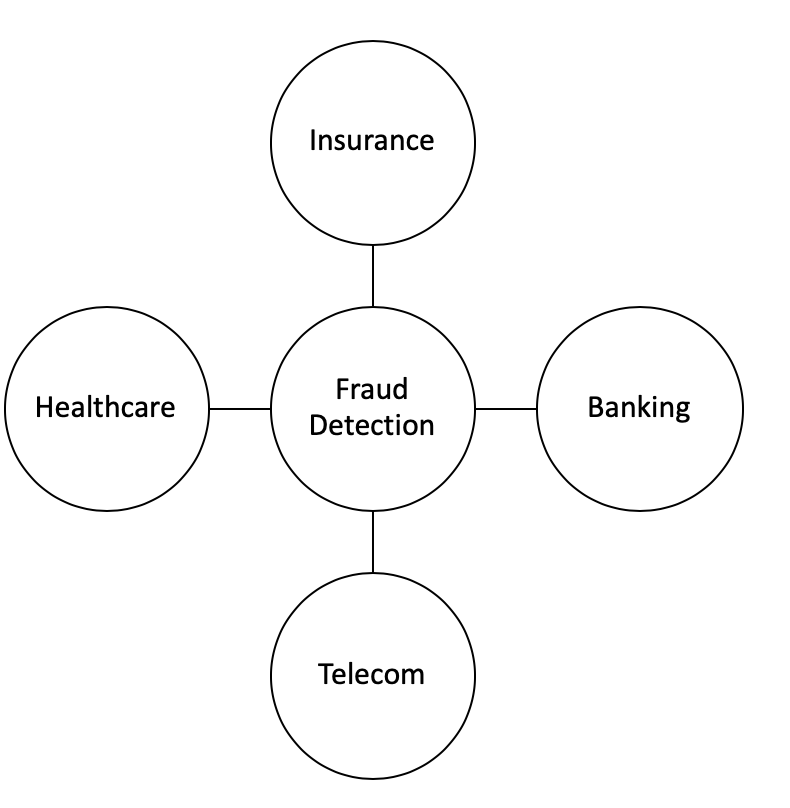
\includegraphics[scale=0.5]{images/AreasOfFraud}
\captionsetup{justification=centering}
\caption{Fraud detection across various application domains.}
\label{fig:AerasOfFraud}
\end{figure}
%%%%%%

Fraud in telecommunications, insurance \textit{( health, automobile, etc)} claims, banking \textit{( tax return claims, credit card transactions etc)} represent significant problems in both governments and private businesses. Detecting and preventing fraud is not a simple task since fraud is an adaptive crime. Many traditional machine learning algorithms have been applied successfully in fraud detection~\cite{sorournejad2016survey}.  The challenge associated with detecting fraud is that it requires real time detection and prevention. This section focuses on deep anomaly detection (DAD) techniques for fraud detection.
%-----------------------------------------------------------------------------------------------------------

\subsubsection{Banking fraud}
In the past decade, credit card was introduced in the banking sector. Now, credit card has become a popular
payment method in online shopping for goods and services. Credit card fraud involves theft of a payment card details, and use it as a fraudulent source of funds in a transaction. Many techniques for credit card fraud detection have been presented in the last few years~\cite{zhou2018state},~\cite{suganya2015survey}. We will briefly review some of DAD techniques as shown Table~\ref{tab:creditfraudDetect}.
The challenge in credit card fraud detection is that frauds have no constant patterns. The typical approach in credit card fraud detection is to maintain a usage profile for each user and monitor the user profiles to detect any deviations. Since there are billions of credit card users this technique of user profile approach is not very scalable. Owing to the inherent scalable nature of DAD techniques, these techniques are gaining wide spread adoption in credit card fraud detection.
%%%%%%% Begin table fraud detection
\begin{table*}
\begin{center}
  \caption{Examples of DAD techniques used in  credit card fraud detection.
          \\AE: Autoencoders, LSTM : Long Short Term Memory Networks
          \\RBM: Restricted Botlzmann Machines, DNN : Deep Neural Networks
          \\GRU: Gated Recurrent Unit, RNN: Recurrent Neural Networks
          \\CNN: Convolutional Neural Networks,VAE: Variational Autoencoders
          \\GAN: Generative Adversarial Networks}
  \captionsetup{justification=centering}
  \label{tab:creditfraudDetect}
  \scalebox{0.83}{
    \begin{tabular}{ | l | p{3cm} | p{10cm} |}
    \hline
    Technique Used & Section & References \\ \hline
     AE  & Section ~\ref{sec:ae}  & ~\cite{schreyer2017detection},~\cite{wedge2017solving} ,~\cite{paula2016deep},~\cite{renstrom2018fraud},~\cite{kazemi2017using},~\cite{zheng2018one},~\cite{pumsirirat2018credit} \\\hline
     RBM  & Section ~\ref{sec:dnn}  & ~\cite{pumsirirat2018credit} \\\hline
     DBN & Section ~\ref{sec:dnn} & ~\cite{seeja2014fraudminer} \\\hline
     VAE & Section ~\ref{sec:gan_adversarial} & ~\cite{sweers2018autoencoding} \\\hline
     GAN & Section ~\ref{sec:gan_adversarial} & ~\cite{fiore2017using},~\cite{choi2018generative} \\\hline
     DNN  & Section ~\ref{sec:dnn} & ~\cite{dorronsoro1997neural}, ~\cite{gomez2018end} \\\hline
     LSTM,RNN,GRU  & Section ~\ref{sec:rnn_lstm_gru} & ~\cite{wiese2009credit}, ~\cite{jurgovsky2018sequence},~\cite{heryadi2017learning},~\cite{ando2016detecting},~\cite{wang2017session},~\cite{alowais2012credit},~\cite{amarasinghe2018critical},~\cite{abroyan2017neural},~\cite{lp2018transaction}\\\hline
     CNN  & Section ~\ref{sec:cnn} & ~\cite{shen2007application},~\cite{chouiekh2018convnets},~\cite{abroyan2017convolutional},~\cite{fu2016credit},~\cite{lu2017deep},~\cite{wang2018credit},~\cite{abroyan2017neural} ,~\cite{zhang2018model}\\\hline
    \end{tabular}}
\end{center}
\end{table*}
%%%%%%%%% End of table Banking detection

%------------------------------------------------------
\subsubsection{Mobile cellular network fraud}
\label{sec:mobilefraud}

In recent times, mobile cellular networks  have witnessed  rapid deployment and evolution
supporting billions of users and a vast diverse array of mobile devices.
Due to this wide adoption and low mobile cellular service rates mobile
cellular networks is now faced with frauds such as voice scams targeted to steal customer private information, and messaging related scams to extort money from customers. Detecting such fraud is of paramount interest and not an easy task due to volume and velocity of mobile cellular network.
Traditional machine learning methods with static feature engineering  techniques fail to adapt to the nature of evolving fraud.
Table ~\ref{tab:mobilefraudDetect} lists DAD techniques for mobile cellular network fraud detection.

%%%%%%% Begin table fraud detection
\begin{table*}
\begin{center}
  \caption{Examples of DAD techniques used in  mobile cellular network fraud detection.
          \\CNN:  convolution neural networks,DBN: Deep Belief Networks
          \\SAE: Stacked Autoencoders, DNN : Deep neural networks
          \\GAN: Generative Adversarial Networks }
  \captionsetup{justification=centering}
  \label{tab:mobilefraudDetect}
  \scalebox{0.9}{
    \begin{tabular}{ | l | p{4cm} | p{5cm} | p{5cm} |}
    \hline
    Technique Used & Section & References \\ \hline
     CNN    & Section ~\ref{sec:cnn}  & ~\cite{chouiekh2018convnets} \\\hline
     SAE, DBN    & Section \ref{sec:ae},~\ref{sec:dnn}   &  ~\cite{alsheikh2016mobile},~\cite{badhe2017click} \\\hline
     DNN & Section ~\ref{sec:dnn}  &  ~\cite{akhter2012detecting},~\cite{jain2017perspective} \\\hline
     GAN & Section ~\ref{sec:gan_adversarial} &  ~\cite{zheng2018generative} \\\hline
    \end{tabular}}
\end{center}
\end{table*}
%%%%%%%%% End of table fraud detection
%-----------------------------------------------------------------------------------------------------------
\subsubsection{Insurance fraud}
Several traditional machine learning methods have been applied successfully to detect fraud in insurance claims ~\cite{joudaki2015using,roy2017detecting}. The traditional approach for fraud detection is based on features which are fraud indicators. The challenge with these traditional approaches is that the need of manual expertise to extract robust features. Another challenge is insurance fraud detection is the that the incidence of frauds is far less than the total number of claims, and also each fraud is unique in its own way. In order to overcome these limitations several DAD techniques are proposed which are illustrated in Table ~\ref{tab:insurancefraudDetect}

%%%%%%% Begin table fraud detection
\begin{table*}
\begin{center}
  \caption{Examples of DAD techniques used in insurance fraud detection.
          \\DBN: Deep Belief Networks, DNN : Deep Neural Networks
          \\CNN: Convolutional Neural Networks,VAE: Variational Autoencoders
          \\GAN: Generative Adversarial Networks}
  \label{tab:insurancefraudDetect}
  \captionsetup{justification=centering}
  \scalebox{0.85}{
    \begin{tabular}{ | l | p{4cm} | p{4cm} | p{4cm} |}
    \hline
     DBN & Section ~\ref{sec:dnn} & ~\cite{viaene2005auto} \\\hline
     VAE & Section ~\ref{sec:gan_adversarial} & ~\cite{fajardo2018vos} \\\hline
     GAN & Section ~\ref{sec:gan_adversarial} & ~\cite{fiore2017using},~\cite{choi2018generative} \\\hline
     DNN & Section ~\ref{sec:dnn} &~\cite{keung2009neural}\\\hline
     CNN  & Section ~\ref{sec:cnn} & ~\cite{shen2007application},~\cite{zhang2018model}\\\hline
    \end{tabular}}
\end{center}
\end{table*}
%%%%%%%%% End of Insurance fraud
% \ref{sec:dnn}
% \ref{sec:stn}
% \ref{sec:spn}
% \ref{sec:word2vec}
% \ref{sec:gan_adversarial}
% \ref{sec:cnn}
% \ref{sec:rnn_lstm_gru}
% \ref{sec:ae}
%-----------------------------------------------------------------------------------------------------------
\subsubsection{Healthcare fraud}

Healthcare is an integral component in people's lives, waste, abuse and fraud drive up costs in healthcare by tens of billions of dollars each year. Healthcare insurance claims fraud is a major contributor to increased healthcare costs, but its impact can be mitigated through fraud detection. Several machine learning models have been used effectively in health care insurance fraud~\cite{bauder2017medicare}.
Table~\ref{tab:healthcarefraudDetect} presents the overview of DAD methods for health-care fraud identification.


%%%%%%% Begin table fraud detection
\begin{table*}
\begin{center}
  \caption{Examples of DAD techniques used in  healthcare fraud detection.
          \\RBM: Restricted Botlzmann Machines, GAN: Generative Adversarial Networks}
  \captionsetup{justification=centering}
  \label{tab:healthcarefraudDetect}
  \scalebox{0.9}{
    \begin{tabular}{ | l | p{4cm} | p{5cm} | p{5cm} |}
    \hline
    Technique Used & Section & References \\ \hline
     RBM & Section ~\ref{sec:dnn} & ~\cite{lasaga2018deep} \\\hline
     GAN & Section ~\ref{sec:gan_adversarial} & ~\cite{ghasedi2018semi},~\cite{finlayson2018adversarial}\\\hline
     CNN  & Section ~\ref{sec:cnn} & ~\cite{esteva2017dermatologist}\\\hline
    \end{tabular}}
\end{center}
\end{table*}
%%%%%%%%% End of table health care fraud
%---------------------------------------------------------------------------------------------------

\label{sec:fraudDetection}

%!TEX root = ../../main.tex
\subsection{Malware Detection}
\label{sec:malwaredetection}

Malware, short for Malicious Software. In  order to protect legitimate users from malware, machine learning based efficient malware detection methods are proposed~\cite{ye2017survey}. In the classical machine learning methods, the process of malware detection is usually divided into two stages: feature extraction and classification/clustering. The performance of traditional malware detection approaches critically depend on the extracted features and the methods for classification/clustering. The challenge associated in malware detection problems is the seer scale of data, for instance considering data as bytes a certain  sequence classification problem could be  of the order of two million time steps. Furthermore the malware is very adpative in nature, wherein the attackers would use advanced techniques to hide the malicious behaviour. Some DAD techniques  which address these challenges effectively and detect malware are shown in Table~\ref{tab:malwareDetect}.

\begin{table*}
  \begin{center}
   \caption{Examples of DAD techniques used for malware detection.
             \\AE: Autoencoders, LSTM : Long Short Term Memory Networks
             \\RBM: Restricted Botlzmann Machines, DNN : Deep Neural Networks
             \\GRU: Gated Recurrent Unit, RNN: Recurrent Neural Networks
             \\CNN: Convolutional Neural Networks,VAE: Variational Autoencoders
             \\GAN: Generative Adversarial Networks,CNN-BiLSTM: CNN- Bidirectional LSTM}
    \captionsetup{justification=centering}
    \label{tab:malwareDetect}
    \scalebox{0.85}{
    \begin{tabular}{|p{3cm}|p{2cm}|p{10cm}|}
      \hline
      \textbf{Technique Used} & \textbf{Section} & \textbf{References}\\
      \hline
      AE &  Section ~\ref{sec:ae}  & ~\cite{yousefi2017autoencoder},~\cite{hardy2016dl4md},~\cite{yousefi2017autoencoder},~\cite{de2018malware},~\cite{sewak2018investigation},~\cite{kebede2017classification},~\cite{de2018malware},~\cite{david2015deepsign}\\\hline
      word2vec & Section ~\ref{sec:word2vec} &  ~\cite{cakir2018malware},~\cite{silva2018improving}\\\hline
      CNN & Section ~\ref{sec:cnn} &  ~\cite{kolosnjaji2018adversarial},~\cite{suciu2018exploring},~\cite{srisakaokul2018muldef},~\cite{srisakaokul2018muldef},~\cite{king2018artificial},~\cite{huang2017r2},~\cite{guo2017malware},~\cite{abdelsalam2018malware},\newline ~\cite{raff2017malware},~\cite{karbab2018maldozer},~\cite{martinelli2017evaluating},~\cite{mclaughlin2017deep},~\cite{gibert2018using},~\cite{kolosnjaji2017empowering}\\\hline
      DNN & Section ~\ref{sec:dnn} &  ~\cite{rosenberg2018end},~\cite{wang2017adversary}\\\hline
      DBN & Section ~\ref{sec:dnn} &  ~\cite{david2015deepsign},~\cite{yang2016application},~\cite{ding2016application},~\cite{yuxin2017malware},~\cite{selvaganapathy2018deep},~\cite{yuxin2017malware},~\cite{hou2017deep}\\\hline
      LSTM & Section ~\ref{sec:rnn_lstm_gru} &  ~\cite{tobiyama2016malware}, ~\cite{hu2017black},~\cite{tobiyama2018method} ,~\cite{passalislong} \\\hline
      CNN-BiLSTM& Section ~\ref{sec:cnn},~\ref{sec:rnn_lstm_gru} &  ~\cite{le2018deep},~\cite{wang2017adversary} \\\hline
      GAN& Section ~\ref{sec:gan_adversarial} &  ~\cite{kim2018zero} \\\hline
      Hybrid model(AE-CNN),(AE-DBN) & Section ~\ref{sec:hybridModels} &  ~\cite{wang2018effective},~\cite{li2015hybrid} \\\hline
      RNN & Section ~\ref{sec:rnn_lstm_gru} &  ~\cite{haddadpajouh2018deep} \\\hline
    \end{tabular}}
  \end{center}
\end{table*}



% OCSVM~\cite{scholkopf2002support}, SVDD~\cite{scholkopf2002support}
% SVM~\cite{cortes1995support}
% KNN~\cite{altman1992introduction}
% Random Forest~\cite{ho1995random}
% Relief~\cite{kira1992feature}
% CSI~\cite{ruchansky2017csi}
% \ref{sec:dnn}
% \ref{sec:stn}
% \ref{sec:spn}
% \ref{sec:word2vec}
% \ref{sec:gan_adversarial}
% \ref{sec:cnn}
% \ref{sec:rnn_lstm_gru}
% \ref{sec:ae}





\label{sec:malwareDetection}

%!TEX root = ../../main.tex
\subsection{Medical Anomaly Detection:}
\label{sec:medical_anomaly_detection}

 Several studies have been conducted to understand the theoretical and practical applications of deep learning in medical and bio-informatics ~\cite{min2017deep,cao2018deep,zhao2016deep,khan2018review}. Finding rare events (anomalies) in areas such as medical image analysis, clinical electroencephalography (EEG) records,  enable to diagnose and provide preventive treatments for a variety of medical conditions. Deep learning based architectures are employed with great success to detect medical anomalies as illustrated in Table ~\ref{tab:medicalanomalyDetect}. The vast amount of imbalanced data in medical domain presents significant challenges to detect  outliers. Additionally deep learning techniques for long have been considered as black-box techniques, i,e even though deep learning models produce outstanding performance, these models lack interpret-ability. In recent times models with good interpret-ability are proposed and shown to produce state-of-the-art performance ~\cite{gugulothusparse,amarasinghe2018toward,choi2018doctor}.

%%%%%%% Begin table fraud detection
\begin{table*}
\begin{center}
  \caption{Examples of DAD techniques Used for medical anomaly detection.
          \\AE: Autoencoders, LSTM : Long Short Term Memory Networks
          \\GRU: Gated Recurrent Unit, RNN: Recurrent Neural Networks
          \\CNN: Convolutional Neural Networks,VAE: Variational Autoencoders
          \\GAN: Generative Adversarial Networks, KNN: K-nearest neighbours
          \\RBM: Restricted Boltzmann Machines.}
  \captionsetup{justification=centering}
  \label{tab:medicalanomalyDetect}
   \scalebox{0.9}{
    \begin{tabular}{ | l | p{3cm} | p{9cm} |}
    \hline
    Technique Used & Section & References \\ \hline
     AE  & Section~\ref{sec:ae} & ~\cite{wang2016research,cowton2018combined},~\cite{sato2018primitive}\\\hline
     DBN & Section~\ref{sec:dnn} & ~\cite{turner2014deep},~\cite{sharma2016abnormality},~\cite{wulsin2010semi},~\cite{ma2018unsupervised},~\cite{zhang2016automatic},~\cite{wulsin2011modeling} ,~\cite{wu2015adaptive}\\\hline
     RBM & Section~\ref{sec:dnn}  & ~\cite{liao2016enhanced}\\\hline
     VAE & Section~\ref{sec:gan_adversarial} & ~\cite{xu2018unsupervised},~\cite{lu2018anomaly} \\\hline
     GAN & Section~\ref{sec:gan_adversarial}&~\cite{ghasedi2018semi},~\cite{chen2018unsupervised} \\\hline
     LSTM ,RNN,GRU & Section~\ref{sec:rnn_lstm_gru} & ~\cite{yang2018toward},~\cite{jagannatha2016bidirectional},~\cite{cowton2018combined},~\cite{o2016recurrent},~\cite{latif2018phonocardiographic},~\cite{zhang2018time},~\cite{chauhan2015anomaly},~\cite{gugulothusparse,amarasinghe2018toward}\\\hline
     CNN  & Section~\ref{sec:cnn} & ~\cite{schmidt2018artificial},~\cite{esteva2017dermatologist},~\cite{wang2016research},~\cite{iakovidis2018detecting}\\\hline
     Hybrid( AE+ KNN) & Section~\ref{sec:cnn} & ~\cite{song2017hybrid} \\\hline
    \end{tabular}}
\end{center}
\end{table*}
%%%%%%%%% End of table Medical anomaly detection








\label{sec:medicalAnomalyDetect}


%!TEX root = ../../main.tex
\subsection{Deep learning for Anomaly detection in Social Networks}
In recent times, online social networks has become part and parcel of daily life. Anomalies in social network
are irregular often unlawful behaviour pattern of individuals within a social network, such  individuals may be identified as  spammers, sexual predators, online fraudsters, fake users or rumour-mongers. Detecting these irregular patterns is of prime importance since if not detected, the act of such individuals can have serious social impact. A survey of traditional anomaly detection techniques and its challenges to detect anomalies in social networks is a well studied topic in literature ~\cite{liu2017social,savage2014anomaly,anand2017anomaly,yu2016survey,cao2018automatic,yu2016survey}. The heterogeneous and dynamic nature of data presents significant challenges to DAD techniques. Despite these challenges several DAD techniques illustrated in Table ~\ref{tab:socialNetworkAnomalyDetect} are shown outperform state-of-the-art methods.

% Table
\begin{table*}
  \begin{center}
   \caption{Examples of DAD techniques used to detect anomalies in social network.
            \\CNN: Convolution Neural Networks, LSTM : Long Short Term Memory Networks
            \\AE: Autoencoders, DAE: Denoising Autoencoders
            \\SVM : Support Vector Machines., DNN : Deep Neural Network  }
    \captionsetup{justification=centering}
    \label{tab:socialNetworkAnomalyDetect}
    \scalebox{0.85}{
    \begin{tabular}{|p{3cm}|p{4cm}|p{5cm}|}
      \hline
      \textbf{Technique Used} & \textbf{Section} & \textbf{References}\\
      \hline
      AE,DAE &  Section ~\ref{sec:ae}  & ~\cite{zhang2017detecting},~\cite{castellini2017fake}\\\hline
      CNN-LSTM & Section ~\ref{sec:cnn}, ~\ref{sec:rnn_lstm_gru} & ~\cite{sun2018detecting},~\cite{shu2017doc},~\cite{yang2018anomaly}\\\hline
      DNN & Section ~\ref{sec:dnn}  & ~\cite{li2017detecting}\\\hline
      Hybrid Models (CNN-LSTM-SVM) & Section ~\ref{sec:hybridModels}  & ~\cite{wei2017new}\\\hline
    \end{tabular}}
  \end{center}
\end{table*}





% Science is a belief in the ingnorance of experts
% Measure of ignorance; Data Artist
% Find Worst Case: Piano
%New Ideas in Business and Intelligence and customer analytics
%Learn the rules like a professional but break like an artist

\label{sec:socialNetworks}


%!TEX root = ../../main.tex
\subsection{Log Anomaly Detection:}
Anomaly detection in log file aims to find text, which can indicate the reasons and the nature of failure of a system. Most commonly, a domain  specific regular-expression  is constructed from past experience which finds new faults by pattern matching. The limitation of such approaches is that newer messages of failures are easily are not detected~\cite{memon2008log}.

The unstructured and diversity in both format and semantics of log data pose significant challenges to log anomaly detection. Anomaly detection techniques should adapt to concurrent setting of log data generated and detect outliers in real time. Following the success of deep neural networks in real time text analysis, several DAD techniques illustrated in Table~\ref{tab:logAnomalyDetect} which model the log data as natural language sequence are shown very effective in detecting outliers.

%%%%%%% Begin table fraud detection
\begin{table*}
\begin{center}
\caption{Examples of Deep learning anomaly detection techniques used in system logs.
        \\CNN: Convolution Neural Networks, LSTM : Long Short Term Memory Networks
        \\GRU: Gated Recurrent Unit, DNN : Deep Neural Networks
        \\AE: Autoencoders, DAE: Denoising Autoencoders}
    \captionsetup{justification=centering}
  \label{tab:logAnomalyDetect}
  \scalebox{0.85}{
    \begin{tabular}{ | p{2cm} | p{2cm} | p{9cm} |}
    \hline
     \textbf{Techniques}  & \textbf{Section} & \textbf{References} \\ \hline
     LSTM & Section ~\ref{sec:rnn_lstm_gru} & ~\cite{hochreiter1997long},~\cite{brown2018recurrent},~\cite{tuor2017deep},~\cite{das2018desh},~\cite{malhotra2015long} \\\hline
     AE & Section ~\ref{sec:ae} & ~\cite{du2017deeplog},~\cite{andrews2016detecting} ,~\cite{sakurada2014anomaly},~\cite{nolle2018analyzing},~\cite{nolle2016unsupervised}\\\hline
     LSTM-AE & Section ~\ref{sec:rnn_lstm_gru}, ~\ref{sec:ae} & ~\cite{grover2018anomaly},~\cite{wolpher2018anomaly} \\\hline
     RNN & Section ~\ref{sec:rnn_lstm_gru} & ~\cite{brown2018recurrent},~\cite{zhang2018role},~\cite{nanduri2016anomaly},~\cite{fengming2017anomaly}\\\hline
     DAE & Section ~\ref{sec:ae} & ~\cite{marchi2015non},~\cite{nolle2016unsupervised}\\\hline
     CNN & Section ~\ref{sec:cnn} & ~\cite{lu2018detecting},~\cite{yuan2018insider},~\cite{racki2018compact},~\cite{zhou2016spatial},~\cite{gorokhov2017convolutional},~\cite{liao2017deep},~\cite{cheng2017deep},~\cite{zhang2018alphamex}\\\hline
    \end{tabular}}
\end{center}
\end{table*}
%%%%%%%%% End of Log anomaly detection











\label{sec:logAnomaly}


%!TEX root = ../../main.tex
\subsection{Internet of things (IoT) Big Data Anomaly Detection}

IoT is identified as a network of  devices that is interconnected with soft-wares, servers, sensors and etc. In the field of Internet of things (IoT), data generated by weather stations, Radio-frequency identification (RFID) tags, IT infrastructure
components, and some other sensors are mostly time series sequential data. Anomaly detection in these IoT networks identifies fraudulent, faulty behaviour of these massive scale of interconnected devices. The challenges associated  in outlier detection is that heterogeneous devices are interconnected which renders the system more complex. A thorough overview on using  deep learning (DL), to facilitate the analytics and learning in the IoT domain is presented by ~\cite{mohammadi2018deep}. In this section we present some of the DAD techniques used in this domain in Table ~\ref{tab:iotBigDataAnomalyDetect}.

%%%%%%% Begin table iot BigData Anomaly Detect
\begin{table*}
\begin{center}
\caption{Examples of DAD techniques used in Internet of things (IoT) Big Data Anomaly Detection.
        \\ AE: Autoencoders, LSTM : Long Short Term Memory Networks
        \\ DBN : Deep Belief Networks.}
 \captionsetup{justification=centering}
  \label{tab:iotBigDataAnomalyDetect}
  \scalebox{0.95}{
    \begin{tabular}{ | l | p{4cm} | p{5cm} |}
    \hline
     \textbf{Techniques}  & \textbf{Section} & \textbf{References} \\ \hline
     AE & Section ~\ref{sec:ae} & ~\cite{luo2018distributed},~\cite{mohammadi2018neural} \\\hline
     DBN & Section ~\ref{sec:dnn} & ~\cite{kakanakova2017outlier} \\ \hline
     LSTM & Section ~\ref{sec:rnn_lstm_gru} & ~\cite{zhang2018lstm},~\cite{mudassar2018unsupervised}\\ \hline
    \end{tabular}}
\end{center}
\end{table*}
%%%%%%%%% End of iot BigData Anomaly Detect






\label{sec:iotBigDataAnomaly}

%!TEX root = ../../main.tex
\subsection{Industrial Anomalies Detection}

Industrial systems consisting of wind turbines, power plants, high-temperature energy systems, storage devices and  with rotating mechanical parts are exposed to enormous stress on a day-to-day basis. Damage to these type of systems not only causes economic loss but also a loss of reputation, therefore detecting and repairing them early is of utmost importance. Several machine learning techniques have been used to detect such damage in industrial systems ~\cite{ramotsoela2018survey,marti2015anomaly}. Several papers published utilizing deep learning models for detecting early industrial damage show great promise~\cite{atha2018evaluation,de2018automatic,wang2018residential}. Damages caused to equipment's are rare events, thus  detecting such events can be formulated as outlier detection problem. The challenges associated with outlier detection in this domain is both volume as well as dynamic nature of data, since failure can be caused due to variety of factors. Some of the DAD techniques employed across various industries are illustrated in Table ~\ref{tab:industrialDamageDetect}.



%%%%%%% Begin table industrial damage detection
\begin{table*}
\begin{center}
\caption{Examples of DAD techniques used in industrial operations.
        \\CNN: Convolution Neural Networks, LSTM : Long Short Term Memory Networks
        \\GRU: Gated Recurrent Unit, DNN : Deep Neural Networks
        \\AE: Autoencoders, DAE: Denoising Autoencoders, SVM: Support Vector Machines
        \\SDAE: Stacked Denoising Autoencoders, RNN : Recurrent Neural Networks.}
    \label{tab:industrialDamageDetect}
    \captionsetup{justification=centering}
    \scalebox{0.85}{
    \begin{tabular}{ | l | p{2cm} | p{8cm} |}
    \hline
     \textbf{Techniques}  & \textbf{Section} & \textbf{References} \\ \hline
     LSTM & Section ~\ref{sec:rnn_lstm_gru} &  ~\cite{inoue2017anomaly},~\cite{thi2017one},~\cite{kravchik2018detecting},~\cite{huang2018deep},~\cite{park2018lired},~\cite{chang2018review}\\\hline
     AE & Section ~\ref{sec:ae} & ~\cite{yuan2015distributed},~\cite{araya2017ensemble},~\cite{qu2017detection},~\cite{sakurada2014anomaly},~\cite{bhattad2018detecting}\\\hline
     DNN & Section ~\ref{sec:dnn} & ~\cite{lodhi2017power}\\\hline
     CNN & Section ~\ref{sec:cnn} & ~\cite{faghih2016deep},~\cite{christiansen2016deepanomaly},~\cite{lee2016convolutional},~\cite{faghih2016deep}, ~\cite{dong2016camera},~\cite{nanduri2016anomaly},~\cite{fuentes2017robust},~\cite{huang2018deep},~\cite{chang2018review}\\\hline
     SDAE,DAE & Section ~\ref{sec:ae} & ~\cite{yan2015accurate},~\cite{luo2017gas},~\cite{dai2017cleaning} \\\hline
     RNN & Section ~\ref{sec:rnn_lstm_gru} & ~\cite{banjanovic2017neural},~\cite{thi2017one} \\\hline
     Hybrid Models (DNN-SVM) & Section ~\ref{sec:hybridModels} & ~\cite{inoue2017anomaly} \\\hline
    \end{tabular}}
\end{center}
\end{table*}
%%%%%%%%% End of industrial damage detection












\label{sec:industrialDamageDetect}

%!TEX root = ../../main.tex
\subsection{Anomaly Detection in Time Series }
\label{sec:timeseriesAD}
Data recorded continuously over a duration is known the time series. Time series data are the best examples of collective outliers. In recent times, deep learning models for detecting time series anomalies has been well studied~\cite{fawaz2018deep,langkvist2014review,gamboa2017deep,lu2017unsupervised}. The advancements in deep learning domain offer opportunities to extract rich hierarchical features which can greatly improve outlier detection as illustrated by various techniques illustrated in Table ~\ref{tab:sensorAnomalyDetect}. Furthermore DeepAD, an anomaly detection framework to detect anomalies precisely, even in complex data patterns is proposed by~\cite{buda2018deepad}. Some of the challenges to detect anomalies in time series using deep learning models data are:
\begin{itemize}
    \item Lack of defined pattern in which an anomaly occuring may be defined.
    \item Noise within the input data seriously effects the performance of algorithms.
    \item As the length of the time series data increases the computational complexity also increases.
    \item Time series data is usually non-stationary, non-linear and dynamically evolving, hence DAD models should be able to detect anomalies in real time.
\end{itemize}


%%%%%%% Begin table sensor networks time series anomaly detection
\begin{table*}
\begin{center}
\caption{Examples of DAD techniques used in time series data.
        \\CNN: Convolution Neural Networks, GAN: Generative Adversarial networks,LSTM : Long Short Term Memory Networks
        \\GRU: Gated Recurrent Unit, DNN : Deep Neural Networks,
        \\AE: Autoencoders, DAE: Denoising Autoencoders, VAE: Variational Autoencoder
        \\ SDAE: Stacked Denoising Autoencoders}
    \captionsetup{justification=centering}
  \label{tab:sensorAnomalyDetect}
  \scalebox{0.90}{
    \begin{tabular}{ | p{3cm} | p{4cm} | p{9cm} |}
    \hline
    \textbf{Techniques}  & \textbf{Section} & \textbf{References} \\ \hline
     LSTM & Section ~\ref{sec:rnn_lstm_gru} & \cite{shipmon2017time},\cite{hundman2018detecting},\cite{zhu2017deep},\cite{hundman2018detecting},\cite{malhotra2015long},\cite{chauhan2015anomaly},\cite{assendorp2017deep},\cite{buda2018deepad},\newline \cite{ahmad2017unsupervised},\cite{malhotra2016lstm},\cite{bontemps2016collective},\cite{taylor2016anomaly},\cite{cheng2016ms},\cite{loganathan2018sequence},\cite{chauhan2015anomaly},\cite{malhotra2015long},\cite{gorokhov2017convolutional}\\\hline
     AE,LSTM-AE,CNN-AE,GRU-AE & Section ~\ref{sec:ae} & ~\cite{Dominique},~\cite{kieu2018outlier},~\cite{cowton2018combined},~\cite{malhotra2016multi},~\cite{malhotra2016lstm},\newline ~\cite{filonov2016multivariate},~\cite{sugimoto2018deep},~\cite{oh2018residual},~\cite{ebrahimzadehmulti}\\\hline
     RNN & Section ~\ref{sec:rnn_lstm_gru} & ~\cite{wielgosz2017recurrent},~\cite{saurav2018online},~\cite{wielgosz2018model},~\cite{guo2016robust}\\\hline
     CNN, CNN-LSTM & Section ~\ref{sec:cnn},~\ref{sec:rnn_lstm_gru} & ~\cite{kanarachos2017detecting},~\cite{dumodeling},~\cite{gorokhov2017convolutional},~\cite{napoletano2018anomaly},~\cite{shanmugam2018jiffy},\cite{medel2016anomaly}\\\hline
     LSTM-VAE & Section ~\ref{sec:rnn_lstm_gru},~\ref{sec:gan_adversarial} & ~\cite{park2018multimodal},~\cite{solch2016variational}\\\hline
     DNN &Section ~\ref{sec:dnn} & ~\cite{amarasinghe2018toward}\\\hline
     GAN &Section ~\ref{sec:gan_adversarial} & ~\cite{li2018anomaly},~\cite{zenati2018efficient},~\cite{lim2018doping},~\cite{laptevanogen}\\\hline
    \end{tabular}}
\end{center}
\end{table*}
%%%%%%%%% End of time series anomaly detection


\label{sec:sensorNetworkAnomaly}


%!TEX root = ../../main.tex

%%%%%%% Begin table for video survellienace anomaly detection
\begin{table*}
\begin{center}
\caption{Examples of DAD techniques used in video surveillance.
        \\CNN: Convolution Neural Networks, LSTM : Long Short Term Memory Networks
        \\RBM: Restricted Boltzmann Machine, DNN : Deep Neural Networks
        \\AE: Autoencoders, DAE: Denoising Autoencoders
        \\OCSVM: One class Support vector machines, CAE: Convolutional Autoencoders
        \\SDAE: Stacked Denoising Autoencoders, STN : Spatial Transformer Networks }
  \label{tab:videoSurvellianceAnomalyDetect}
  \captionsetup{justification=centering}
  \scalebox{0.80}{
    \begin{tabular}{ | p{3cm} | p{4cm} | p{12cm} |}
      \hline
      \textbf{Technique Used} & \textbf{Section} & \textbf{References}\\
      \hline
      CNN & Section ~\ref{sec:cnn} & \cite{dong2016camera},\cite{andrewsaanomaly},\cite{sabokrou2016fully},\cite{sabokrou2017deep},\cite{munawar2017spatio},\cite{li2017transferred},\cite{qiao2017abnormal},\cite{tripathi2018convolutional},\cite{nogas2018deepfall},\cite{christiansen2016deepanomaly},\cite{li2017transferred}\\\hline
      SAE (AE-CNN-LSTM)  &  Section ~\ref{sec:ae},~\ref{sec:cnn},~\ref{sec:rnn_lstm_gru}  & ~\cite{chong2017abnormal},~\cite{qiao2017abnormal},~\cite{khaleghi2018improved}\\\hline
      AE &  Section ~\ref{sec:ae}  & \cite{qiao2017abnormal},\cite{yang2015unsupervised},\cite{chen2015detecting},\cite{gutoskidetection},\cite{d2017autoencoder},\cite{dotti2017unsupervised},\cite{yang2015unsupervised},\cite{chen2015detecting},\cite{sabokrou2016video},\cite{tran2017anomaly},\cite{chen2015detecting} ,\cite{d2017autoencoder},\cite{hasan2016learning},\cite{yang2015unsupervised},\cite{cinelli2017anomaly}\\\hline
      Hybrid Model (CAE-OCSVM) & Section ~\ref{sec:hybridModels}  & ~\cite{gutoskidetection}, ~\cite{dotti2017unsupervised}\\\hline
      LSTM-AE &  Section ~\ref{sec:rnn_lstm_gru}, ~\ref{sec:ae}  & ~\cite{d2017autoencoder}\\\hline
      STN &Section~\ref{sec:stn}   & \cite{chianucci2016unsupervised}\\\hline
      RBM &Section ~\ref{sec:dnn}   & \cite{munawar2017spatio}\\\hline
      LSTM &Section ~\ref{sec:rnn_lstm_gru}  &~\cite{medel2016anomaly},~\cite{luo2017remembering},~\cite{ben2018attentioned},~\cite{singh2017anomaly}\\\hline
      RNN & Section ~\ref{sec:rnn_lstm_gru} &\cite{luo2017revisit},\cite{zhou2015abnormal} ,\cite{hu2016video},~\cite{chong2015modeling}\\\hline
      AAE & Section ~\ref{sec:gan_adversarial} & ~\cite{ravanbakhsh2017training}\\\hline
    \end{tabular}}
  \end{center}
\end{table*}
%%%%%%%%% End of video survellienace anomaly detection


\subsection{Video Surveillance}
Video Surveillance also popularly known as Closed-circuit television (CCTV) involves monitoring a designated areas of interest in order to ensure security. In videos surveillance applications unlabelled data is available in large amounts, this is a significant challenge for supervised machine learning and deep learning methods. Hence video surveillance applications have been modelled as anomaly detection problems owing to lack of availability of labelled data. Several works have studied the state-of-the-art deep models for video anomaly detection and  have classified them based on the type of model and criteria of detection~\cite{kiran2018overview,chong2015modeling}. The challenges of robust 24/7 video surveillance systems is discussed in detail by Boghossian et.al~\cite{boghossian2005challenges}. The lack of  explicit definition of anomaly in real-life video surveillance is a significant issue that hampers the performance of DAD methods as well. DAD techniques used in  video surveillance  are illustrated  in Table ~\ref{tab:videoSurvellianceAnomalyDetect}.







% % Datasets Used Table
% \begin{table*}
%   \begin{center}
%     \caption{Datasets Used For Video surveillance}
%     \label{tab:videoSurvelliance}
%     \begin{tabular}{|p{3cm}|p{4cm}|p{6cm}|}
%       \hline
%       \textbf{DataSet} & \textbf{Type} & \textbf{References}\\
%       \hline
%       UCSD Ped2~\cite{ucsdAnomalyDetect2017},Subway~\cite{adam2008robust} &  Video   & Sabokrou et al~\cite{sabokrou2016fully,sabokrou2017deep}, Gutoski et al~\cite{gutoskidetection} \\ \hline
%       LOST ~\cite{Abrams et al. 2012} &  Video   & Dotti et al~\cite{dotti2017unsupervised}\\ \hline
%       YouTube &  Video   & Yang et al~\cite{yang2015unsupervised}\\ \hline
%       UMN~\footnote{$http://mha.cs.umn.edu$} &  Video   & Sabokrou et al~\cite{yang2015unsupervised}\\ \hline
%       CIFAR-10 &Images& Munawar et al~\cite{munawar2017spatio} \\ \hline
%     \end{tabular}
%   \end{center}
% \end{table*}
% %%%%%%%%% End of Datasets used in video survellienace anomaly detection



































\label{sec:videoSurvelliance}












%!TEX root = ../main.tex
\section{Deep Anomaly Detection (DAD) Models}
\label{sec:deepDADModels}

In this section we discuss various DAD models classified  based on availability of labels and training objective. For each model types domain we discuss the following four aspects:\\
\textemdash assumptions;\\
\textemdash type of model architectures;\\
\textemdash computational complexity;\\
\textemdash advantages and disadvantages;\\

%!TEX root = ../../main.tex
\subsection{Supervised deep anomaly detection}
\label{sec:supervisedDAD}
 Supervised anomaly detection techniques are superior in performance compared to unsupervised anomaly detection techniques  since these techniques use  labeled samples.~\cite{gornitz2013toward}.  Supervised anomaly detection learns the separating boundary from a set of annotated data instances (training) and then, classify a test instance into  either normal or anomalous classes with the learned model (testing).\\
\textbf{Assumptions :}
Deep supervised learning methods depend on separating data classes whereas unsupervised
techniques focus on explaining and understanding the characteristics of data. Multi-class classification based anomaly detection techniques assume that the training data contains labeled instances of  multiple normal classes ~\cite{shilton2013combined,jumutc2014multi,kim2015deep,erfani2017shared}. Multi-class anomaly detection techniques learn a classifier to distinguish between anomalous class from the rest of the classes. In general, supervised deep learning-based classification schemes for anomaly detection have two sub-networks, a feature extraction network followed by a classifier network. Deep models require extremely large number of training samples (in the order of thousands or millions) to effectively learn feature representations to discriminate various class instances. Due to, lack of availability of clean data labels supervised deep anomaly detection techniques are not so popular as semi-supervised and unsupervised methods.

\textbf{Computational Complexity :} 
The computational complexity of deep supervised  anomaly detection methods based techniques depends on the  input data dimension and the number of hidden layers trained using back-propagation algorithm. High dimensional data tend to have more hidden layers to ensure meaning-full hierarchical learning of input features.The computational complexity also increases  linearly with the number of hidden layers and require greater model training and update time.


\textbf{Advantages and Disadvantages :}
The advantages of supervised DAD techniques are as follows:
\begin{itemize}
\item Supervised DAD methods are more accurate than semi-supervised and unsupervised models.
\item The testing phase of classification based techniques is fast since each test instance
needs to be compared against the pre-computed model.
\end{itemize}
The disadvantages of Supervised DAD techniques are as follows:
\begin{itemize}
\item  Multi-class supervised techniques require accurate labels for various normal classes and anomalous instances, which is often not available.
\item Deep supervised techniques fail to separate normal from anomalous data , if the feature space is highly complex and non-linear.
\end{itemize}













\label{sec:supervised}

%!TEX root = ../../main.tex
\subsection{Semi-supervised deep anomaly detection }
\label{sec:semi_supervised_DAD}
Semi-supervised or (one-class classification) DAD techniques assume that all training instances have only one class label.  A review of deep learning based semi-supervised techniques is presented by Kiran et.al and Min et.al~\cite{kiran2018overview,min2018ids}. DAD techniques learn a discriminative boundary around the normal instances. The test instance that does not belong to the majority class is flagged as being anomalous~\cite{perera2018learning,blanchard2010semi}. Various  semi-supervised DAD model architectures are illustrated in Table~\ref{tab:semisupervisedModels}.

%%%%%%% Begin table Semi-supervised deep anomaly detection models
\begin{table*}
\begin{center}
\caption{Semi-supervised DAD models overview
        \\AE: Autoencoders, DAE: Denoising Autoencoders, KNN : K- Nearest Neighbours
        \\CorGAN: Corrupted Generative Adversarial Networks, DBN: Deep Belief Networks
        \\ AAE: Adversarial Autoencoders, CNN: Convolution neural networks
        \\ SVM:  Support vector machines.}
    \label{tab:semisupervisedModels}
    \begin{tabular}{ | p{4cm} | p{4cm} | p{4cm} |}
    \hline
     \textbf{Techniques}  & \textbf{Section} & \textbf{References} \\ \hline
     AE & Section ~\ref{sec:ae} & ~\cite{edmunds2017deep} ,~\cite{estiri2018semi}\\\hline
     RBM & Section ~\ref{sec:dnn} & ~\cite{jia2014novel} \\\hline
     DBN & Section ~\ref{sec:dnn} & ~\cite{wulsin2010semi},~\cite{wulsin2011modeling} \\\hline
     CorGAN,GAN & Section~\ref{sec:gan_adversarial} & ~\cite{gu2018semi} ~\cite{akcay2018ganomaly},~\cite{sabokrou2018adversarially}\\\hline
     AAE &Section~\ref{sec:gan_adversarial} & ~\cite{dimokranitou2017adversarial}\\\hline
     Hybrid Models (DAE-KNN~\cite{altman1992introduction}), (DBN-Random Forest~\cite{ho1995random}),CNN-Relief~\cite{kira1992feature},CNN-SVM~\cite{cortes1995support} & Section~\ref{sec:DHM} & ~\cite{song2017hybrid},~\cite{shi2017semi},~\cite{zhu2018hybrid} \\\hline
     CNN & Section~\ref{sec:cnn} & ~\cite{racah2017extremeweather},~\cite{perera2018learning} \\ \hline
     RNN & Section~\ref{sec:rnn_lstm_gru} & ~\cite{wu2018semi} \\ \hline
     GAN & Section~\ref{sec:gan_adversarial} & ~\cite{kliger2018novelty},~\cite{gu2018semi} \\ \hline
    \end{tabular}
\end{center}
\end{table*}
%%%%%%%%% End of industrial damage detection

% OCSVM~\cite{scholkopf2002support}, SVDD~\cite{scholkopf2002support}
% SVM~\cite{cortes1995support}
% KNN~\cite{altman1992introduction}
% Random Forest~\cite{ho1995random}
% Relief~\cite{kira1992feature}
% CSI~\cite{ruchansky2017csi}
% Section ~\ref{sec:ae}
% Section ~\ref{sec:rnn_lstm_gru}
% Section ~\ref{sec:gan_adversarial}
% Section ~\ref{sec:dnn}
% Section ~\ref{sec:cnn}
% Section ~\ref{sec:hybridModels}


\textbf{Assumptions : }
Semi-supervised DAD methods proposed rely on one the following assumptions to score a data instance as an anomaly.
\begin{itemize}
 \item  Proximity and Continuity: Points which are close to each other both in input space  and learnt feature space are more likely to share a same label.
  \item Robust features are learnt within hidden layers of deep neural network layers and retain the discriminative attributes for separating normal from outlier data points.
\end{itemize}

\textbf{Computational Complexity :} 
The computational complexity of semi-supervised DAD methods based techniques is similar to supervised DAD techniques, which primarily depends on the dimensionality of the input data and the number of hidden layers used for representative feature learning.\\

\textbf{Advantages and Disadvantages:}
The advantages of semi-supervised deep anomaly detection techniques are as follows:
\begin{itemize}
\item  Generative Adversarial Networks (GANs) trained in semi-supervised learning mode have shown great promise, even with very few labeled data.
\item  Use of labeled data ( usually of one class), can produce considerable performance improvement   over unsupervised techniques.
\end{itemize}
The fundamental disadvantages of semi-supervised techniques presented by Lu et.al ~\cite{lu2009fundamental} is applicable even in deep learning context. Furthermore the hierarchical features extracted within hidden layers may not be representative of fewer anomalous instances hence are prone to over-fitting problem.











\label{sec:semiSupervised}

%!TEX root = ../../main.tex


%%%%%%% Begin table industrial damage detection
\begin{table*}
\begin{center}
\caption{Examples of  Hybrid DAD techniques.
        \\CNN: Convolution Neural Networks, LSTM : Long Short Term Memory Networks
        \\DBN: Deep Belief Networks, DNN : Deep Neural Networks.
        \\AE: Autoencoders, DAE: Denoising Autoencoders, SVM: Support Vector Machines~\cite{cortes1995support}
        \\SVDD: Support Vector Data Description, RNN : Recurrent Neural Networks
        \\Relief: Feature selection Algorithm~\cite{kira1992feature}, KNN: K- Nearest Neighbours~\cite{altman1992introduction}
        \\CSI: Capture, Score, and Integrate~\cite{ruchansky2017csi}. }
    \captionsetup{justification=centering}
    \label{tab:hybridModels}
    \scalebox{0.85}{
    \begin{tabular}{ | p{3cm} | p{2cm} | p{6cm} |}
    \hline
     \textbf{Techniques}  & \textbf{Section} & \textbf{References} \\ \hline
     AE-OCSVM, AE-SVM & Section ~\ref{sec:ae}, & ~\cite{andrews2016detecting} \\\hline
     DBN-SVDD, AE-SVDD & Section ~\ref{sec:dnn}, & ~\cite{erfani2016high},~\cite{kim2015deep} \\\hline
     DNN-SVM & 21D & ~\cite{inoue2017anomaly} \\\hline
     DAE-KNN, DBN-Random Forest~\cite{ho1995random},CNN-Relief,CNN-SVM & Section ~\ref{sec:dnn},\ref{sec:ae} & ~\cite{song2017hybrid},~\cite{shi2017semi},~\cite{zhu2018hybrid,urbanowicz2018relief} \\\hline
     AE-CNN, AE-DBN & Section ~\ref{sec:dnn},~\ref{sec:cnn},\ref{sec:ae} &  ~\cite{wang2018effective},~\cite{li2015hybrid} \\\hline
     AE+ KNN & Section \ref{sec:ae} & ~\cite{song2017hybrid} \\\hline
     CNN-LSTM-SVM & Section ~\ref{sec:cnn},\ref{sec:rnn_lstm_gru}  & ~\cite{wei2017new}\\
     RNN-CSI & Section ~\ref{sec:rnn_lstm_gru} & ~\cite{ruchansky2017csi}\\
     CAE-OCSVM & Section \ref{sec:ae} & ~\cite{gutoskidetection}, ~\cite{dotti2017unsupervised}\\\hline
    \end{tabular}}
\end{center}
\end{table*}

\subsection{Hybrid deep anomaly detection}
\label{sec:hybridModels}
Deep learning models are widely used as feature extractors to learn robust features~\cite{andrews2016detecting}. In hybrid deep models, the representative features learnt within deep models are input to traditional algorithms like one-class Radial Basis Function (RBF) , Support Vector Machine (SVM) classifiers. The hybrid models employ two step learning and are shown to produce state-of-the-art results~\cite{erfani2016high,erfani2016robust,wu2015harvesting}.  Deep hybrid architectures used in anomaly detection are illustrated in Table ~\ref{tab:hybridModels}.

%%%%%%%%% End of Hybrid Models

% OCSVM~\cite{scholkopf2002support}, SVDD~\cite{scholkopf2002support}
% SVM~\cite{cortes1995support}
% KNN~\cite{altman1992introduction}
% Random Forest~\cite{ho1995random}
% Relief~\cite{kira1992feature}
% CSI~\cite{ruchansky2017csi}
% Section ~\ref{sec:ae}
% Section ~\ref{sec:rnn_lstm_gru}
% Section ~\ref{sec:gan_adversarial}
% Section ~\ref{sec:dnn}
% Section ~\ref{sec:cnn}
% Section ~\ref{sec:stn}
% Section ~\ref{sec:hybridModels}



\textbf{Assumptions : } \\
The deep hybrid models proposed for anomaly detection rely on one the following assumptions to detect outliers:
\begin{itemize}
  \item Robust features are extracted within hidden layers of deep neural network, aid in separating out the irrelevant features which can conceal the presence of anomalies.
  \item Building a robust anomaly detection model on complex, high-dimensional spaces require feature extractor and an anomaly detector. Various anomaly detectors used alongwith are illustrated in Table ~\ref{tab:hybridModels}
\end{itemize}

\textbf{Computational Complexity :} \\
Computational complexity of an hybrid model includes complexity of both deep architectures as well as traditional algorithms used within.  Additionally  an inherent issue of non-trivial choice of deep network architecture and parameters which involves searching optimized parameters in a considerably larger space introduces the computational complexity of using deep layers within hybrid models. Furthermore considering the classical algorithms such as  linear SVM which has prediction complexity  of $O(d)$ with d the number of input dimensions. For most kernels, including polynomial and RBF, the complexity is $O(nd)$ where $n$ is the number of support vectors although an approximation $O(d^2)$ is considered for SVMs with an RBF kernel.

\textbf{Advantages and Disadvantages }\\
The advantages of hybrid DAD techniques are as follows:
\begin{itemize}
\item  The feature extractor greatly reduce the ‘curse of dimensionality’ especially in high dimensional domain.
\item  Hybrid models are  more scalable and computationally efficient since the linear or nonlinear kernel models operate on reduced input dimension.
\end{itemize}
The significant disadvantages of hybrid DAD techniques are:
\begin{itemize}
\item  The hybrid approach is suboptimal because it is unable to influence representational learning within the hidden layers of feature extractor, since generic loss functions are employed instead of  customised objective for anomaly detection.
\item The deeper hybrid models tend to perform better, if the individual layers are pre-trained ~\cite{saxe2011random} which introduces computational expenditure.
\end{itemize}













\label{sec:hybrid}

%!TEX root = ../../main.tex
\subsection{One-class neural networks (OC-NN) for anomaly detection}
\label{sec:oneclassNN}
One-class neural networks (OC-NN) combines the ability of deep networks to extract progressively rich representation of data alongwith the one-class objective, such as an hyperplane~\cite{chalapathy2018anomaly} or hypersphere ~\cite{ruff2018deep} to separate all the normal data points from the outliers. The OC-NN approach is novel for the following crucial reason: data representation in the hidden layer are learned by optimising the objective function customised for anomaly detection as illustrated in
The experimental results in ~\cite{chalapathy2018anomaly,ruff2018deep} demonstrate that OC-NN can achieve comparable or better performance than existing state-of-the art methods for complex datasets, while having reasonable training and testing time compared to the existing methods.

\textbf{Assumptions : } 
The OC-NN models proposed for anomaly detection rely on the  following assumptions to detect outliers:
\begin{itemize}
 \item  OC-NN models extracts the common factors of variation within the data distribution within the hidden layers of deep neural network.
  \item Performs combined representation learning and produces a outlier score for test data instance.
  \item Anomalous samples do not contain common factors of variation and hence hidden layers fails to capture the representations of outliers.
\end{itemize}

\textbf{Computational Complexity :} 
The Computational complexity of an OC-NN model as against the  hybrid model includes only the complexity of deep network of choice ~\cite{saxe2011random}. OC-NN models do not require  data to be
stored for prediction, thus have very low memory complexity. However  it is evident that the OC-NN training time is proportional to the input dimension.

\textbf{Advantages and Disadvantages:}
The advantages of OC-NN  are as follows:
\begin{itemize}
\item  OC-NN  models jointly trains a deep neural network while optimizing a data-enclosing hypersphere or hyperplane in output space.
\item OC-NN propose an alternating minimization algorithm for learning
the parameters of the OC-NN model. We observe that the subproblem of the OC-NN objective is equivalent to a solving a quantile selection problem which is well defined.
\end{itemize}
The significant disadvantages of OC-NN for anomaly detection are:
\begin{itemize}
\item Training times  and model update time may be longer for high dimensional input data.
\item Model updates would also take longer time, given the change in input space.
\end{itemize}



\label{sec:oneClassNeuralNetworks}

%!TEX root = ../../main.tex
\subsection{Unsupervised Deep Anomaly Detection }
\label{sec:unsupervisedDAD}
Unsupervised DAD is an important area of research  in both fundamental machine learning research and industrial applications. Several deep learning frameworks that addresses  challenges in unsupervised anomaly detection are proposed and shown to produce state-of-the-art performance as illustrated in Table ~\ref{tab:unsupervisedAnomalyDetection}. Autoencoders are the fundamental  unsupervised deep architectures used in anomaly detection~\cite{baldi2012autoencoders}.

%%%%%%% Begin Un-supervised Deep Anomaly Detection (UDAD)
\begin{table*}
\begin{center}
\caption{Examples of  Un-supervised DAD techniques .
        \\CNN: Convolution Neural Networks, LSTM : Long Short Term Memory Networks
        \\DNN : Deep Neural Networks., GAN: Generative Adversarial Network
        \\AE: Autoencoders, DAE: Denoising Autoencoders, SVM: Support Vector Machines
        \\STN: Spatial Transformer Networks, RNN : Recurrent Neural Networks
        \\AAE: Adversarial Autoencoders, VAE : Variational Autoencoders.}
\captionsetup{justification=centering}
    \label{tab:unsupervisedAnomalyDetection}
    \scalebox{0.85}{
    \begin{tabular}{ | p{3cm}  | p{2cm} | p{8cm} |}
    \hline
     \textbf{Techniques}  & \textbf{Section} & \textbf{References} \\ \hline
     LSTM & Section ~\ref{sec:rnn_lstm_gru} &  ~\cite{singh2017anomaly},~\cite{chandola2008comparative},~\cite{dasigi2014modeling},\cite{malhotra2015long}\\\hline
     AE & Section ~\ref{sec:ae} & ~\cite{abati2018and},~\cite{zong2018deep},~\cite{tagawa2015structured},~\cite{dau2014anomaly},~\cite{sakurada2014anomaly},~\cite{wu2015adaptive},\newline~\cite{xu2015learning},~\cite{hawkins2002outlier},~\cite{zhao2015robust},~\cite{qi2014robust},~\cite{chalapathy2017robust},~\cite{yang2015unsupervised},\newline ~\cite{zhai2016deep},~\cite{lyudchik2016outlier},~\cite{lu2017unsupervised},~\cite{mehrotra2017deep},~\cite{meng2018relational},\cite{parchami2017using}\\\hline
     STN & Section ~\ref{sec:stn} & ~\cite{chianucci2016unsupervised}\\\hline
     GAN & Section ~\ref{sec:gan_adversarial} & ~\cite{lawson2017finding} \\\hline
     RNN & Section ~\ref{sec:rnn_lstm_gru} & ~\cite{dasigi2014modeling},\cite{filonov2017rnn} \\\hline
     AAE & Section ~\ref{sec:gan_adversarial} & ~\cite{dimokranitou2017adversarial},~\cite{leveau2017adversarial} \\\hline
     VAE & Section ~\ref{sec:gan_adversarial} &  ~\cite{an2015variational},~\cite{suh2016echo},~\cite{solch2016variational},~\cite{xu2018unsupervised},~\cite{mishra2017generative}\\\hline
    \end{tabular}}
\end{center}
\end{table*}
%%%%%%%%% End of Un-supervised Deep Anomaly Detection (UDAD)

% OCSVM~\cite{scholkopf2002support}, SVDD~\cite{scholkopf2002support}
% SVM~\cite{cortes1995support}
% KNN~\cite{altman1992introduction}
% Random Forest~\cite{ho1995random}
% Relief~\cite{kira1992feature}
% CSI~\cite{ruchansky2017csi}
% Section ~\ref{sec:ae}
% Section ~\ref{sec:rnn_lstm_gru}
% Section ~\ref{sec:gan_adversarial}
% Section ~\ref{sec:dnn}
% Section ~\ref{sec:cnn}
% Section ~\ref{sec:stn}
% Section ~\ref{sec:hybridModels}

\textbf{Assumptions : } 
The deep unsupervised models proposed for anomaly detection rely on one the following assumptions to detect outliers:
\begin{itemize}
 \item The “normal” regions in the original or some latent feature space can be distinguished from "anomalous" regions in the original or some latent feature space.
  \item The majority of the data instances are normal compared to the remainder of the data set.
  \item Unsupervised anomaly detection algorithm produces an outlier score of the data instances based on  intrinsic properties of the data-set such as distances or densities. The hidden layers of deep neural network aim to capture these intrinsic properties within the dataset~\cite{goldstein2016comparative}.
\end{itemize}

\textbf{Computational Complexity :} 
The autoencoders is the most common architecture employed in outlier detection with quadratic cost, the optimization problem is non-convex in nature, similar to any other neural network architecture.
The model computational complexity depends on the number of operations, network parameters and hidden layers. However, the computational complexity of training an autoencoder is much higher than traditional methods such as Principal Component Analysis (PCA) since PCA is
based on matrix decomposition ~\cite{meng2018relational,parchami2017using}.\\

\textbf{Advantages and Disadvantages:}
The advantages of unsupervised deep anomaly detection techniques are as follows:
\begin{itemize}
\item  Learns the inherent data characteristics to separate normal from anomalous data point. These technique  identifies commonalities within the data therefore facilitates outlier detection.
\item  Cost effective technique to find the anomalies since it does not require annotated data for training the algorithms.
\end{itemize}
The significant disadvantages of unsupervised deep anomaly detection techniques are:
\begin{itemize}
\item  Often it is difficult to learn commonalities within data in a complex and high dimensional space.
\item While using autoencoders the choice of right degree of compression, i.e. dimensionality reduction is often an hyper-parameter that requires tuning for optimal results.
\item Unsupervised techniques techniques are very sensitive to noise, and data corruptions and
       are often less accurate than supervised or semi-supervised techniques.
\end{itemize}









\label{sec:unsupervised}

%!TEX root = ../../main.tex
\subsection{Miscellaneous Techniques}
This section explores, various DAD techniques which are shown to be effective and promising,  we discuss the key idea behind those techniques, and their area of applicability.

\subsubsection{Transfer Learning based anomaly detection : }
Deep learning for long has been critized for the need to have enough data to produce good results.
Transfer learning relaxes this data dependence and helps to  achieve good performance even with limited  training data instances. Litjens et.al and Pan et.al ~\cite{litjens2017survey,pan2010survey} present the review on deep transfer learning approaches. Transfer learning is an important tool in machine learning to solve the basic problem of insufficient training data. It aims to transfer the knowledge from the source domain to the target domain by relaxing the assumption that  training and future data must be in the same feature space and have the same distribution. Deep transfer representation-learning has been explored ~\cite{andrews2016transfer,vercruyssen2017transfer,li2012detecting,almajai2012anomaly,kumar2017transfer,liang2018transfer} and shown to produce very promising results. The open research questions using transfer learning for anomaly detection is , the degree of  transferability, that is to define how well features transfer the knowledge and improve the classification performance from one task to another.

\subsubsection{Zero Shot learning based anomaly detection:}
Zero shot learning (ZSL)  aims recognize objects never seen before within training set~\cite{romera2015embarrassingly}.
ZSL achieves this  in two phases: Firstly the  knowledge about the objects in natural language descriptions or attributes (commonly known as meta-data) is captured Secondly this knowledge is then used to classify instances among a new set of classes. This setting is important in real world since one may not be able to obtain images of all the possible classes at training. The main challenge associated with this approach is the obtaining the meta-data about the data instances. However several approaches of using ZSL in anomaly and novelty detection are shown to produce state-of-the-art results ~\cite{mishra2017generative,socher2013zero,xian2017zero,liu2017generalized,rivero2017grassmannian}.

\subsubsection{Ensemble based anomaly detection:}
 A notable issue with deep neural networks is that they are sensitive to noise within input data and often require large training data to perform robustly~\cite{kim2016lstm}. In order to achieve robustness even in noisy data an idea to randomly vary on the connectivity architecture of the autoencoder are shown to obtain signicantly better performance. An autoencoder ensembles consisting of  various randomly connected autoencoders are experimented by Chen et.al ~\cite{chen2017outlier} to achieve promising results on several bench-mark datasets. The ensemble approaches are still an active area of research which has been shown to produce improved diversity, thus avoid overfitting problem while reducing training time.

% Similarly Kim et.al  employ a novel ensemble method that combines  multiple thresholding classifiers into a single one unit , enabling it possible to recognize ‘highly normal’ sequences.

\subsubsection{Clustering based anomaly detection:}
Several anomaly detection  algorithms based on clustering have been proposed in literature ~\cite{ester1996density}. Clustering involves grouping together similar patterns based on features extracted  detect new anomalies. The time and space complexity grows linearly with number of classes to be clustered ~\cite{sreekanth2010generalized}, which renders the clustering based anomaly detection prohibitive for real-time practical applications.  The dimensionality of the input data is reduced  extracting features within the hidden layers of deep neural network which ensures scalability for complex and high dimensional datasets.  Deep learning enabled clustering approach anomaly detection utilizes e.g word2vec ~\cite{mikolov2013efficient}  models to get the semantical presentations of normal data and anomalies to form clusters and detect outliers ~\cite{yuan2017deep}. Several works rely on variants of hybrid models along with auto-encoders for obtaining representative features for  clustering to find anomalies~\cite{aytekin2018clustering,xie2016unsupervised,guo2017improved,xie2016unsupervised,guo2017deep,wang2016learning,mani2018scalable}.


\subsubsection{Deep Reinforcement Learning (DRL) based anomaly detection:}
\label{reinforcementlearning},
Deep reinforcement learning (DRL) methods have attracted significant interest due to its ability to learn complex behaviors in high-dimensional data space. Efforts to detect anomalies using deep reinforcement learning have been proposed by ~\cite{de2017learning,rlanomaly}.
The DRL based anomaly detector  does not consider any assumption about the concept of the anomaly,  the detector identifies new anomalies by consistently enhancing its knowledge  through reward signals accumulated. DRL based anomaly detection is a very novel concept which  requires further investigation and identification of research gap and its applications.

\subsubsection{Statistical techniques deep anomaly detection: }
Hilbert transform is statistical signal processing technique which derives the analytic representation of a real-valued signal. This property is leveraged by Kanarachos et.al~\cite{kanarachos2015anomaly} for real time detection of anomalies in health related time series dataset and is shown to be a very promising technique. The algorithm combines the ability of wavelet analysis, neural networks and Hilbert transform in a sequential manner to detect real-time anomalies. The topic of statistical techniques DAD techniques requires further investigation to fully understand thier potential and applicability for anomaly detections.


% Although the authors claim the real time detection of anomalies In the fourth comming years these statistical signal processing techniques have been rarely experimented due to the fact that the training phase can be computationally demanding and exprensive.


\label{sec:others}

%!TEX root = ../main.tex
\section{Deep neural network architectures for locating anomalies}
\label{sec:locatingAnomalieswithNNArchitecture}


\subsection{Deep Neural Networks (DNN)}
\label{sec:dnn}
The "deep" in "deep neural networks" refers to the number of layers through which the features of data are extracted~\cite{schmidhuber2015deep,bengio2009learning}. Deep architectures overcome the limitations of traditional machine learning approaches of scalability, and generalization to new variations within data~\cite{lecun2015deep} and the need for manual feature engineering. Deep Belief Networks (DBNs) are class of deep neural network which comprises of multiple layer of graphical models known as Restricted Boltzmann Machine (RBMs).
The hypothesis in using DBNs for anomaly detection is that RBMs are used as  directed encoder-decoder network that can be trained with backpropogation algorithm~\cite{werbos1990backpropagation}. DBNs fail to capture the common variations of anomalous samples, resulting in high reconstruction error. DBNs  are shown to scale efficiently to big-data and improve interpretability~\cite{wulsin2010semi}.


\subsection{Spatio Temporal Networks (STN)}
\label{sec:stn}
Researchers for long have explored  techniques to learn both both spatial and temporal relation features~\cite{zhang2018detecting}. Deep learning architectures have been shown perform well at learning spatial aspects ( using CNNs) and temporal features ( using LSTMs) individually. Spatio Temporal Networks (STNs) comprise of deep neural architectures combining both CNNs and LSTMs to extract spatio-temporal features. The temporal
features (modeling correlations between near time points via LSTM), spatial features (modeling
local spatial correlation via local CNNs) are shown to be effective in detecting outliers~\cite{lee2018stan,szeker2014spatio,nie2018spatio,dereszynski2011spatiotemporal}.

\subsection{ Sum-Product Networks (SPN)}
\label{sec:spn}
Sum-Product Networks (SPNs) are directed acyclic graphs with variables as leaves, and the internal nodes, and weighted edges constitute the sums and products. SPNs are considered as a combination of mixture models  which have fast exact probabilistic inference over many layers~\cite{poon2011sum,peharz2018probabilistic}. The main advantage of SPNs is that, unlike graphical models, SPNs are more traceable over high treewidth models without requiring approximate inference. Furthermore, SPNs are shown to capture uncertainty over their inputs in a convincing manner, yielding robust anomaly detection~\cite{peharz2018probabilistic}. SPNs are shown to be  impressive results on numerous datasets, while much remains to be further explored in relation to outlier detection.

\subsection{Word2vec Models}
\label{sec:word2vec}
Word2vec is a group of deep neural network models used to produce word embeddings~\cite{mikolov2013efficient}. These models are capable of capturing sequential relationships within  data instance such as sentences, time sequence data. Obtaining word embedding features as inputs is shown to improve the performance in several deep learning architectures~\cite{rezaeinia2017improving,naili2017comparative,altszyler2016comparative}. Anomaly detection models leveraging the word2vec embeddings are shown to significantly improve performance. ~\cite{schnabel2015evaluation,bertero2017experience,bakarov2018anomaly,bamler2017dynamic}.


\subsection{Generative Models }
\label{sec:gan_adversarial}

Generative models aim to learn true data distribution in order to generate new data points with some variations. The two most common and efficient generative approaches are Variational Autoencoders (VAE)~\cite{kingma2013auto} and Generative Adversarial Networks (GAN)~\cite{NIPS2014_5423,goodfellow2014generative}. A variant of GAN architecture known as Adversarial autoencoders (AAE) ~\cite{makhzani2015adversarial} that use adversarial training to impose an arbitrary prior on the latent code learnt within hidden layers of autoencoder are also shown to effectively learn the input distribution. Leveraging this ability of learning input distributions, several Generative Adversarial Networks-based Anomaly Detection (GAN-AD) frameworks ~\cite{li2018anomaly,deecke2018anomaly,schlegl2017unsupervised,ravanbakhsh2017abnormal,eide2018applying}
 proposed are shown to be effective in identifying anomalies on high dimensional and complex datasets. However traditional methods such as K-nearest neighbours (KNN) are shown to perform better in scenarios which have lesser number of anomalies when compared to deep generative models~\cite{vskvara2018generative}.

\subsection{Convolutional Neural Networks }
\label{sec:cnn}
Convolutional Neural Networks (CNNs), are the popular choice of neural networks for analyzing visual imagery~\cite{krizhevsky2012imagenet}.  CNN’s ability to extract complicated hidden features from high dimensional data with complex structure has enabled its use as feature extractors in outlier detection for both sequential and image dataset~\cite{gorokhov2017convolutional,kim2014convolutional}. Evaluation of CNNs based frameworks for anomaly detection is still an active area of research being explored currently~\cite{kwon2018empirical}.

\subsection{Sequence Models}
\label{sec:rnn_lstm_gru}

Recurrent Neural Networks (RNNs)~\cite{williams1989complexity} are shown to capture features of time sequence data. The limitations with RNNs is that they fail to capture the context as time steps increases, in order to resolve this problem,  Long Short-Term Memory~\cite{hochreiter1997long} networks was introduced, they  are a special type of RNNs comprising of memory cell that can store information about previous time steps. Gated Recurrent Unit~\cite{cho2014learning} (GRUs) are similar to LSTMs, but use a set of gates to control the flow of information, instead of separate memory cells.
Anomaly detection in sequential data  has attracted significant interest in literature due its applications in a wide range of engineering problems illustrated in Section ~\ref{sec:timeseriesAD}.
Long Short Term Memory (LSTM) neural network based algorithms for anomaly detection  have been investigated and reported to produce significant performance gains over conventional methods~\cite{ergen2017unsupervised}.

\subsection{Autoencoders}
\label{sec:ae}
Autoencoders with single layer alongwith a linear activation function is nearly equivalent to Principal Component Analysis (PCA)~\cite{pearson1901liii}. While PCA is restricted to a linear dimensionality reduction, auto encoders enable both linear or nonlinear tranformations~\cite{liou2008modeling,liou2014autoencoder}. One of the popular applications of Autoencoders is anomaly detection. Autoencoders represent data within multiple hidden layers by reconstructing the input data, effectively learning an identity function. The autoencoders when trained solely on normal data instances ( which are the majority in anomaly detection tasks) fail to reconstruct the anomalous data samples therefore producing a large reconstruction error. The data samples which produce high residual errors are considered outliers. Several variants of autoencoder architectures are proposed as illustrated in Figure ~\ref{fig:aevariants} produce promising results in anomaly detection. The choice of autoencoder architecture depends on the nature of data, convolution networks are preferred for image datasets while Long short-term memory (LSTM) based models tend to produce good results for sequential data. Efforts to combine both convolution and LSTM layers where encoder is a convolutional neural network (CNN) and decoder is a multilayer LSTM network to reconstruct  input images are shown to be effective in detecting anomalies within data.  The use of combined models  such as Gated recurrent unit autoencoders (GRU-AE), Convolutional neural networks autoencoders (CNN-AE), Long short-term memory (LSTM) autoencoder (LSTM-AE) eliminate the need for preparing hand-crafted features,  and facilitates the use of raw data with minimal preprocessing in anomaly detection tasks.


%%%%% Autoencoder architectures used in anomaly detection %%%%%
\tikzset{edge from parent/.style=
{draw, edge from parent path={(\tikzparentnode.south)
-- +(0,-8pt)
-| (\tikzchildnode)}},
blank/.style={draw=none}}

\begin{figure}
\centering
\begin{tikzpicture}
\matrix
{
% \node{\Tree
%     [A.  \edge[blank];
%     [B.  \edge[blank];
%     [C. \edge[blank];
%     [D. ]]]]};
&
\node{\Tree
 [.Autoencoders
    [.Images
        [{CAE} {CNN-AE}  {CNN-LSTM-AE} {DAE} ] ]
    [.{Sequential Data}
            [ {LSTM-AE} GRU-AE AE SDAE ]]]};\\
};
\end{tikzpicture}
\caption{   {Autoencoder architectures for anomaly detection}.
        \\AE: Autoencoders~\cite{liou2014autoencoder}, LSTM : Long Short Term Memory Networks~\cite{hochreiter1997long}
        \\SDAE: Stacked Denoising Autoencoder~\cite{vincent2010stacked}, DAE : Denoising Autoencoders~\cite{vincent2010stacked}
        \\GRU: Gated Recurrent Unit~\cite{cho2014learning}, CNN: Convolutional Neural Networks~\cite{krizhevsky2012imagenet}
        \\CNN-LSTM-AE: Convolution Long Short Term Memory Autoencoders~\cite{haque2018image}
        \\CAE: Convolutional Autoencoders~\cite{masci2011stacked}
        }

 \label{fig:aevariants}
\end{figure}
Although autoencoders are simple and effective architectures for outlier detection. However, the performance gets degraded  due to noisy training data with a large fraction of corruptions~\cite{zhou2017anomaly}.


%!TEX root = ../main.tex
\section{ Relative Strengths and Weakness : Deep Anomaly Detection Methods}
\label{sec:relativeSOW}
Each of the deep anomaly detection (DAD) techniques discussed in previous
sections have their unique strengths and weaknesses. It is critical to understand which
anomaly detection technique is best suited for a given anomaly detection problem context.
Given the fact that DAD is an active research area, it is not feasible to provide such an
understanding for every anomaly detection problem. Hence in  this section we analyze the
relative strengths and weakenesses of different categories of techniques for a few
simple problem settings.\\
Classification based supervised DAD techniques illustrated in Chapter ~\ref{chpt:supervisedDAD} are  better choices in scenario consisting of equal amount of labels for both normal and anomalous instances. The computational complexity of supervised DAD technique is a key aspect, especially when the technique is applied to a real domain. While classification
based, supervised or semi-supervised techniques have expensive training times, testing is usually fast since it uses pre-trained model. Unsupervised DAD techniques presented in Chapter~\ref{chpt:unsupervisedDAD} are being widely used since
label acquisition is very expensive and time consuming process. Most of the unsupervised deep anomaly detection requires priors to be assumed on the anomaly distribution hence the models are less robust in handling noisy data. Hybrid models illustrated in Section~\ref{sec:hybridModels} extract robust features within hidden layers of deep neural network, and feed to best performing classical anomaly detection algorithms. The hybrid model approach is suboptimal because it is unable to influence representational learning in the hidden layers.  The One-class Neural Networks  (OC-NN) described in Section~\ref{sec:oneclassNN} combines the ability of deep networks to extract progressively rich representation of data alongwith the one-class objective, such as an hyperplane~\cite{chalapathy2018anomaly} or hypersphere ~\cite{ruff2018deep} to separate all the normal data points from the origin. Further research and exploration is necessary to better comprehend the benefits of this new architecture proposed.





% !TEX root=../main.tex
In this paper, we have proposed a one-class neural network (OC-NN) approach for anomaly detection.
OC-NN uses a one-class SVM (OC-SVM) like loss function to train a neural network.
The advantage of OC-NN is that the features of the hidden layers are constructed for the specific
task of anomaly detection. This approach is substantially different from recently proposed
hybrid approaches which use deep learning features as input into an anomaly detector.  Feature
extraction in hybrid approaches is generic and not aware of the anomaly detection task. To learn
the parameters of the OC-NN network we have proposed a novel alternating minimization approach and
have shown that the optimization of a subproblem in OC-NN is equivalent to a quantile selection
% problem. Experiments on complex image and sequential data sets demonstrates that OC-NN is
% highly accurate. For future work, we would like to build and deploy an end to end system for anomaly
% detection based on OC-NN.




% \section{Anomaly detection: motivation and challenges}
% % !TEX root=../main.tex
A common need when analysing real-world datasets is determining which instances stand out as being dissimilar to all others. Such instances are known as \emph{anomalies}, and the goal of \emph{anomaly detection} (also known as \emph{outlier detection}) is to determine all such instances in a data-driven fashion~\cite{chandola2007outlier}. Anomalies can be caused by errors in the data but sometimes are indicative of a new, previously unknown, underlying process; in fact Hawkins~\cite{hawkins1980identification} defines an outlier as an observation that {\it deviates so significantly from other observations as to arouse suspicion that it was generated by a different mechanism.}

Unsupervised anomaly detection techniques uncover anomalies in an unlabeled test data, which plays a pivotal role in a variety of applications, such as, fraud detection, network intrusion detection and fault diagnosis. One-class Support Vector Machines (OC-SVM)~\cite{scholkopf2002support,tax2004support} are widely used, effective unsupervised techniques to identify anomalies. However, performance of OC-SVM is sub-optimal on complex, high dimensional datasets~\cite{vapnik1998statistical,vishwanathan2003simplesvm,bengio2007scaling}.
From recent literature, unsupervised anomaly detection using deep learning is proven to be very effective~\cite{zhou2017anomaly,chalapathy2017robust}. Deep learning methods for anomaly detection can be broadly classified into model architecture using autoencoders~\cite{andrews2016detecting} and hybrid models~\cite{erfani2016high}. Models involving autoencoders utilize magnitude of residual vector (i,e reconstruction error) for making anomaly assessments. While hybrid models mainly use autoencoder as feature extractor, wherein the hidden layer representations are used as input to traditional anomaly detection algorithms such as one-class SVM (OC-SVM). Following the success of transfer learning~\cite{pan2010survey} to obtain rich representative features, hybrid models have adopted pre-trained transfer learning models to obtain features as inputs to anomaly detection methods. Although using generic pre-trained networks for transfer learning representations is efficient, learning representations from scratch, on a moderately sized dataset, for a specific task of anomaly detection is shown to perform better~\cite{andrews2016transfer}. Since the hybrid models extract deep features using an autoencoder and then feed it to a separate anomaly detection method like OC-SVM, they fail to influence representational learning in the hidden layers. In this paper, we build on the theory to integrate a OC-SVM equivalent objective into the neural network architecture. The OC-NN combines the ability of deep networks to extract progressively rich representation of data alongwith the one-class objective, which obtains the hyperplane to separate all the normal data points from the origin. The OC-NN approach is novel for the following crucial reason:  data representation ,is driven by the OC-NN objective and is thus customized for anomaly detection. We show that OC-NN can achieve comparable or better performance in some scenarios than existing shallow state-of-the art methods for complex datasets, while having reasonable training and testing time compared to the existing methods.
%R Hidden layer activations
% in the hidden layer as illustrated in Figure~\ref{fig:h_activations}
% \begin{figure}[t]
%     \centering
%     \includegraphics[width=0.8\textwidth]{images/activations}
%     \caption{Hidden layer (sigmoid) activations and its t-sne~\cite{tSNEVisualize2008} embeddings of OC-NN model for CIFAR-10 dataset.}
%     \label{fig:h_activations}
%     \vspace{-0.530cm}
% \end{figure}

We summarize our main contributions as follows:
\begin{itemize}
\item We derive a new one class neural network (OC-NN) model for anomaly detection. OC-NN uses a one class SVM like loss function to drive the training
of the neural network.
\item We propose an alternating minimization algorithm for learning the parameters of the OC-NN model. We observe that the subproblem of
the OC-NN objective is equivalent to a solving a quantile selection problem.
\item We carry out extensive experiments which convincingly demonstrate  that OC-NN  outperforms other state-of-the-art deep learning approaches
for anomaly detection on complex image and sequence data sets.
\end{itemize}

The rest of the paper is structured as follows. In Section~\ref{sec:background} we provide a detailed survey of related and relevant
work on anomaly detection. The main OC-NN model is developed in Section~\ref{sec:method}. The experiment setup, evaluation metrics and
model configurations are described in Section~\ref{sec:ocnnexperiment-setup}. The results and analysis of the experiments are the focus of
Section~\ref{sec:ocnnexperiment-results}. We conclude in Section~\ref{sec:conclusion} with a summary and directions for future work.



% \section{Background and related work on anomaly detection}
% \label{sec:background}
% \label{sec:related}
% % !TEX root=../main.tex

\begin{comment}
Consider a feature matrix $\X \in \Real^{N \times D}$,
where $N$ denotes the number of data points and $D$ the number of features for each point.
For example, $N$ could be the number of images in some photo collection, and $D$ the number of pixels used to represent each image.
The goal of anomaly detection is to determine which rows of $\X$ are anomalous, in the sense of being dissimilar to all other rows. We will use $\X_{n :}$ to denote the $n$th row of $\X$.
\end{comment}

%\subsection{A tour of anomaly detection methods}

Anomaly detection is a well-studied topic in Data Science~\cite{chandola2007outlier,charubook}. Unsupervised anomaly detection aims at discovering
rules to separate normal and anomalous data in the absence of labels. One-Class SVM (OC-SVM) is a popular unsupervised approach to detect anomalies, which constructs
a smooth boundary around the majority of probability mass of data~\cite{Scholkopf:2001}. OC-SVM will be  described in detail in Section~\ref{sec:ocsvm}.
In recent times, several approaches of feature selection and feature extraction methods have been proposed for complex, high-dimensional
data for use with OC-SVM ~\cite{cao2003comparison,neumann2005combined}.
Following the unprecedented success of using deep autoencoder networks, as feature extractors, in tasks as diverse as visual, speech anomaly detection~\cite{chong2017abnormal,marchi2017deep}, several hybrid models that combine feature extraction using deep learning and OC-SVM
have appeared~\cite{sohaib2017hybrid,erfani2016high}. The benefits of leveraging pre-trained transfer learning  representations for anomaly detection in hybrid models was made evident by the results obtained, using two publicly available~\footnote{Pretrained-models:http://www.vlfeat.org/matconvnet/pretrained/.} pre-trained CNN models: ImageNet-MatConvNet-VGG-F (VGG-F) and  ImageNet-MatConvNet-VGG-M (VGG-M)~\cite{andrews2016transfer}. However, these hybrid OC-SVM approaches are decoupled in the sense that the feature learning is task agnostic and not customized for anomaly detecion. Recently a deep model which trains a neural network by minimizing the volume of a hypersphere that encloses the network representations of the data is proposed ~\cite{pmlrv80ruff18a}, our approach differs from this approach by combining the ability of deep networks to extract progressively rich representation of data alongwith the one-class objective, which obtains the hyperplane to separate all the normal data points from the origin.
 %In this paper, we formulate and evaluate a new architecture for anomaly detection in complex, high-dimensional domains by integrating the one-class objective into neural network arhitecture. The proposed one-class neural network (OC-NN) model is trained using standard back-propogation algorithm to learn, rich differentiable features customized for anomaly detection. To the best of our knowledge, this is the first method proposed which
%combines the ability of deep networks to extract progressively rich representation of data
%with the one-class objective of creating a tight envelope around normal data to improve the performance
%for anomaly detection.

\begin{comment}
\subsection{Deep hybrid OC-SVM Models.}
A popular hybrid approach followed in unsupervised anomaly detection is to couple feature reduction and extraction methods alongwith SVMs~\cite{cao2003comparison,neumann2005combined,shen2008feature,widodo2007combination}. Several hybrid models have been proposed to leverage the representational power of deep learning to address scalability issues of SVMs~\cite{song2017hybrid,you2017hybrid,sohaib2017hybrid}. Deep learning architectures such as sparse stacked autoencoder (SAE)-based deep neural networks (DNNs)~\cite{sohaib2017hybrid}, deep belief networks (DBNs)~\cite{erfani2016high} are adopted for extracting robust features. DBNs are generative models consisting of multiple layers of latent variables ("hidden units"). The advantages of using DBNs are two-fold: (a) their ability to perform non-linear dimensionality reduction (b) learn high dimensional data representations. A DBN can be trained efficiently in a greedy layer-wise fashion by using a Restricted Boltzmann Machine (RBM)~\cite{hinton2010practical}. A Restricted Boltzmann machine model can be defined by joint energy function on the hidden variable $h_k$ with $K$ dimension and visible input variable $x_d$ with $D$ dimension as seen in Equation~\ref{energy}. The model parameters $W^P_{dk}$ encode the pairwise compatibility between $x_d$ and $h_k$ while the  parameters $W^B_k$ and $W^C_d$ are biases which, selectively activates either $h_k$ or $x_d$.

\begin{align}
\label{energy}
    E_W(\mbf{x},\mbf{h})&=
-\sum_{d=1}^D\sum_{k=1}^K W^P_{dk}x_dh_k - \sum_{k=1}^KW^B_k h_k - \sum_{d=1}^D W^C_d x_d
\end{align}

In the context of anomaly detection for images, the $\mbf{x}$ variables may represent (e.g  pixels of the image). The hidden units are binary vector of length $K$ less than original dimension of image $D$. Training an RBM implies finding the values of the parameters such that the energy is minimised. One possible approach is to maximise the log-likelihood of $x$ that is estimated by its gradient with respect to the model parameters using Contrastive Divergence (CD). The DBN consisting of stack of RBMs model encodes rich feature representations of the input within hidden units. While a hybrid model consisting of DBN, trained to extract generic underlying features, as inputs to one-class SVM trained are shown to be effective~\cite{erfani2016high}. The experiments in the aforementioned work were performed on real-datasets comprising 1D inputs, synthetic data or texture images, which have lower dimensionality and different data distribution compared to colour images or long protein sequences.
\end{comment}

%%%%%
\subsection{Robust Deep Autoencoders for anomaly detection}
Besides the hybrid approaches which use OC-SVM with deep learning features another approach for anomaly detection is to use deep autoencoders.
Inspired by RPCA~\cite{xu2010robust}, unsupervised anomaly detection techniques such as robust deep autoencoders can be used to separate
normal from anomalous data~\cite{zhou2017anomaly,chalapathy2017robust}.
Robust Deep Autoencoder (RDA) or Robust Deep Convolutional Autoencoder (RCAE) decompose input data $X$ into two parts $X = L_D + S$, where $L_D$ represents the latent representation the hidden layer of the autoencoder. The matrix  $S$ captures noise and outliers which are hard to reconstruct as shown in Equation~\ref{eqn:robust-ae}. The decomposition is carried out by optimizing the objective function shown in Equation~\ref{eqn:robust-ae}.

\begin{equation}
	\label{eqn:robust-ae}
	\min_{\theta, S} + ||L_D - D_{\theta}(E_{\theta}(L_D)) ||_{2}+ \lambda \cdot \| S^T \|_{2,1}
\end{equation}
 \hspace{1.8cm}   $s.t. \hspace{0.2cm} X - L_D -S = 0 $



The above optimization problem is solved using a combination of backpropagation and Alternating Direction Method of Multipliers (ADMM) approach~\cite{boyd2004convex}. In our experiments  we have carried out a detailed comparision between OC-NN and approaches based on robust autoencoders.

\begin{comment}
Notice that in the constraint of Equation~\ref{eqn:robust-ae} we split the input data X into two
parts, $L_D$ and $S$. $L_D$ is the input to an autoencoder $D_{\theta}(E_{\theta}(L_D))$ and
we train this autoencoder by minimizing the reconstruction error
 $||L_D - D_{\theta}(E_{\theta}(L_D)) ||_{2}$ through back-propagation. $S$, on the other
hand, contains noise and outliers which are learnt applying proximal methods following Alternating Direction Method of Multipliers (ADMM) ~\cite{boyd2004convex}. While $\lambda$ tuning parameter is selected in a semi-supervised fashion through grid-search for optimal $F1$ score.
RDA could be leveraged to detect anomalies similar to OC-SVM setting. The results obtained using our proposed approach of OC-NN are comparable to the results obtained on anomaly detection task on both MNIST and Cifar-10 datasets, as illustrated in Table~\ref{tbl:mnist-usps-anomaly-results-summary} and Table~\ref{tbl:cifar-10-pfam-anomaly-results-summary}.
\end{comment}

\subsection{One-Class SVM for anomaly detection}
\label{sec:ocsvm}

One-Class SVM (OC-SVM) is a widely used approach to discover anomalies in an unsupervised fashion~\cite{scholkopf2002support}. OC-SVMs are a special case of support vector machine, which learns a  hyperplane to separate all the data points from the origin in a reproducing kernel Hilbert space (RKHS) and maximises the distance from this hyperplane to the origin. Intuitively in OC-SVM all the data points are considered as positively labeled instances and the origin
as the only negative labeled instance. More specifically, given a training data $\X$, a set without any class information, and $\Phi(\X)$  a RKHS map function
from the input space to the feature space $F$,  a
hyper-plane or linear decision function $f(\X_{n :})$ in the feature space $F$ is constructed as
$f( \X_{n :} ) = w^T \Phi(\X_{n :}) - \bias$,  to separate as many as possible of the mapped vectors
${ \Phi(\X_{n :}), n: 1,2,...,N}$ from the origin. Here  $w$ is the norm perpendicular to the hyper-plane and $\bias$ is the bias of the hyper-plane. In order to
obtain $w$ and $\bias$, we need to solve the
following optimization problem,

\begin{equation}
\label{eqn:ocsvm-objective}
 \min_{w,\bias} \frac{1}{2} \| w \|_{2}^2+ \frac{1}{\nu} \cdot \frac{1}{N} \sum_{n = 1}^N \max( 0, \bias - \langle w, \Phi(\X_{n :}) \rangle ) - \bias.
\end{equation}

where $\nu \in (0,1)$, is a parameter that
controls a trade off between maximizing the distance of the
hyper-plane from the origin and the number of data points
that are allowed to cross the hyper-plane (the false positives).
%When $\nu$ is small, fewer data fall on the same side of the hyper-plane as the origin in the
%feature space $F$.





% \section{From One Class SVM  to One Class Neural Networks}
% \label{sec:method}
% % !TEX root=../main.tex

We now present our one-class Neural Network (OC-NN) model for unsupervised anomaly detection.
The method can be seen as designing a neural architecture using an  OC-SVM equivalent loss function.
Using OC-NN we will be able to exploit and refine features obtained from unsupervised tranfer learning specifically for anomaly
detection. This in turn will it make it possible to discern anomalies in complex data sets where the decision boundary between normal and anomalous
is highly nonlinear.
\vspace{-0.1cm}
\subsection{One-Class Neural Networks (OC-NN)}
\label{sec:oc-nn}
We design a simple feed forward network with one hiden layer having linear or sigmoid activation $g(\cdot )$ and one output node. Generalizations to deeper
architectures is straightforward. The OC-NN objective can be formulated as:
\begin{equation}
	\label{eqn:oc-nn}
	\min_{w, V, \bias} \frac{1}{2} \| w \|_{2}^2 + \frac{1}{2} \| V \|_F^2 + \frac{1}{\nu} \cdot \frac{1}{N} \sum_{n= 1}^N \max( 0, \bias - \langle w, g( V  \X_{n :} ) \rangle ) - \bias
\end{equation}

where $w$ is the scalar output obtained from the hidden to output layer,
$V$ is the weight matrix from input to hidden units.
Thus the \underline{key insight} of the paper is to replace the dot product $\mathbf{\langle w,\Phi(\X_{n :}) \rangle}$ in OC-SVM with the dot product $\mathbf{\langle w,g(V\X_{n :})\rangle}$. This change will make it possible to leverage transfer learning features obtained using an autoencoder and create an additional layer to refine
the features for anomaly detection. However, the price for the change is that the objective becomes non-convex and thus the resulting algorithm
for inferring the parameters of the model will not lead to a global optima.

%which is randomly initialized from the uniform distribution within the range $[-1, 1]$.  $\nu \in (0,1)$, is the parameter that
%equates to the percentage of anomalies within data, found via grid search in the experiments. $\bias$ is the equivalent maximum margin separating plane from the origin.


%%%%
\begin{comment}
\subsection{Connection to OC-SVM}
\label{sec:connection_to_OC-SVM}

Clearly, Equation~\ref{eqn:oc-nn} is the special case of the Equation~\ref{eqn:ocsvm-objective} presented in the Section~\ref{sec:ocsvm}, where the weights $V$  in Equation~\ref{eqn:oc-nn} are randomly initialised, and not optimised, and $g$ is the either a $linear$ and $sigmoid$ activations.
More generally, for a deep network with parameters $w$, we have

\begin{equation}
\label{eqn:gen-oc-nn}
 \min_{w,\bias} \frac{1}{2} \| w \|_{2}^2 +\frac{1}{\nu} \cdot \frac{1}{N} \sum_{i = 1}^N \max( 0, \bias - \langle w, \Phi( \X_{n :} w ) \rangle ) - \bias
\end{equation}
\end{comment}

%%%%
\vspace{-0.1cm}
\subsection{Training the model}
\label{sec:training}
We can optimize Equation~\ref{eqn:oc-nn} using an alternate minimization approach: We first fix $r$ and optimize for $w$ and $V$. We then use
the new values of $w$ and $V$ to optimize $r$. However, as we  will show, the optimal value of $r$ is just the $\upsilon$-quantile of
the array $\langle w,g(Vx_{n})\rangle$. We first define the objective to solve for $w$ and $V$ as
% \vspace{-0.1cm}
\begin{equation}
                \label{eqn:minimize_w_V}
                 \underset{w, V}{\argmin} \frac{1}{2} \| w \|_{2}^2 + \frac{1}{2} \| V \|_F^2 + \frac{1}{\upsilon} \cdot \frac{1}{N} \sum_{n = 1}^N \ell( y_n, \hat{y}_n( w, V ) )
                 \end{equation}
                where
                \begin{align*}
                        \ell( y, \hat{y} ) &= \max( 0, y - \hat{y} ) \\
                        y_n       &= \bias \\
                        \hat{y}_n( w, V ) &= \langle w, g( V x_n ) \rangle
                \end{align*}

Similarly the optimization problem for $\bias$ is
\begin{equation}
\label{eqn:minimize_r}
\underset{\bias}{\argmin} \left( \frac{1}{N\upsilon} \cdot \sum_{n = 1}^N \max( 0, \bias - \hat{y}_n ) \right) - r
\end{equation}
\begin{comment}
%%%
\begin{enumerate}[(1)]
	\item Initialise $w^{(0)}, V^{(0)}, r^{(0)}$ randomly
	\item for $t = 1, 2, \ldots$
	\begin{enumerate}[(a)]
		\item find $(w^{(t+1)}, V^{(t+1)})$ that minimise the objective through Backpropagation (BP) algorithm.
		\begin{equation}
		\label{eqn:minimize_w_V}
		 \underset{w, V}{\argmin} \frac{1}{2} \| w \|_{2}^2 + \frac{1}{2} \| V \|_F^2 + \frac{1}{\upsilon} \cdot \frac{1}{N} \sum_{n = 1}^N \ell( y_n, \hat{y}_n( w, V ) )
		 \end{equation}
		where
		\begin{align*}
			\ell( y, \hat{y} ) &= \max( 0, y - \hat{y} ) \\
			y_n       &= \bias^{(t)} \\
			\hat{y}_n( w, V ) &= \langle w, g( V x_n ) \rangle
		\end{align*}

		\item pick $\bias^{(t)}$ to be the $\upsilon^{\text{th}}$ quantile of $\{ \hat{y}_n \}_{n = 1}^N$, where
		$$ \hat{y}_n^{(t+1)} = \langle w^{(t+1)}, g( V^{(t+1)} x_n ) \rangle. $$
	\end{enumerate}

\end{enumerate}

To justify step 2(b), let us observe that the optimisation with respect to $\bias$ is\\
%
\begin{equation}
\label{eqn:minimize_r}
\underset{\bias}{\argmin} \left( \frac{1}{N\upsilon} \cdot \sum_{n = 1}^N \max( 0, \bias - \hat{y}_n ) \right) - r
\end{equation}
\end{comment}
\begin{theorem}
Given $w$ and $V$ obtained from solving Equation~\ref{eqn:minimize_w_V}, the solution to Equation~\ref{eqn:minimize_r} is given
by the $\upsilon^{\text{th}}$ quantile of $\{ \hat{y}_n \}_{n = 1}^N$, where
                $$ \hat{y}_n = \langle w, g(V x_n ) \rangle. $$
\end{theorem}
\begin{proof}
 We can rewrite Equation~\ref{eqn:minimize_r} as:
\begin{align*}
%\underset{\bias}{\argmin} \left( \frac{1}{N\upsilon} \cdot \sum_{n = 1}^N \max( 0, \bias - \hat{y}_n ) \right) - r \\
\underset{\bias}{\argmin} \left( \frac{1}{N\upsilon} \cdot \sum_{n = 1}^N \max( 0, \bias - \hat{y}_n ) \right) - \left( \bias - \frac{1}{N} \sum_{n = 1}^{N} \hat{y}_n \right) \\
= \underset{\bias}{\argmin} \left( \frac{1}{N\upsilon} \cdot \sum_{n = 1}^N \max( 0, \bias - \hat{y}_n ) \right) - \left( \frac{1}{N} \sum_{n = 1}^{N} \left[ \bias - \hat{y}_n \right] \right) \\
= \underset{\bias}{\argmin} \left( \sum_{n = 1}^N \max( 0, \bias - \hat{y}_n ) \right) - \upsilon \cdot \left( \sum_{n = 1}^{N} \left[ \bias - \hat{y}_n \right] \right) \\
= \underset{\bias}{\argmin} \sum_{n = 1}^N \left[ \max( 0, \bias - \hat{y}_n ) - \upsilon \cdot \left( \bias - \hat{y}_n \right) \right] \\
= \underset{\bias}{\argmin} \sum_{n = 1}^N
\begin{cases} (1 - \upsilon) \cdot \left( \bias - \hat{y}_n \right) & \text{ if } \bias - \hat{y}_n > 0 \\ - \upsilon \cdot \left( \bias - \hat{y}_n \right) & \text{ otherwise}
\end{cases}
\end{align*}
% \vspace{0.4cm}
\vspace{-0.1cm}
We can observe that the derivative with respect to $r$ is
$$ F'( r ) = \sum_{n = 1}^N \begin{cases} (1 - \upsilon) & \text{ if } \bias - \hat{y}_n > 0 \\ -\upsilon & \text{ otherwise. } \end{cases} $$
Thus, by F'( r ) = 0 we obtain
%
\begin{align*}
	(1 - \upsilon) \cdot \sum_{n = 1}^N \indicator{ \bias - \hat{y}_n > 0 } &= \upsilon \cdot \sum_{n = 1}^N \indicator{ \bias - \hat{y}_n \leq 0 } \\
	&= \upsilon \cdot \sum_{n = 1}^N (1 - \indicator{ \bias - \hat{y}_n > 0 }) \\
	&= \upsilon \cdot N - \upsilon \cdot \sum_{n = 1}^N \indicator{ \bias - \hat{y}_n > 0 },
\end{align*}
or
\begin{equation}
 \frac{1}{N} \sum_{n = 1}^N \indicator{ \bias -\hat{y}_n > 0 }= \frac{1}{N} \sum_{n = 1}^N \indicator{ \hat{y}_n < r } = \upsilon
\end{equation}\\
This means we would require the $\nu^{\text{th}}$ quantile of $\{ \hat{y}_n \}_{n = 1}^N$.
\end{proof}
% \vspace{0.3cm}
%Algorithm
\vspace{-0.3cm}
\subsection{OC-NN Algorithm}
\label{sec:algorithm}
We summarize the solution in Algorithm~\ref{alg1}. We initialize $\bias^{(0)}$ in Line 2. We learn the parameters($w,V$) of the neural network
using the standard Backpropogation(BP) algorithm (Line 7). In the experiment section, we will train the model using features extracted from
an autoencoder instead of raw data points. However this has no impact on the OC-NN algorithm. As show  in Theorem 3.1, we solve for $\bias$
using the $\upsilon$-quantile of the scores $\langle y_{n} \rangle$. Once the convergence criterion is satisfied, the data points are
labeled normal or anomalous using the decision function $S_{n} = sgn(\hat{y}_{n} - r)$.

\begin{algorithm}
\caption{one-class neural network (OC-NN) algorithm}\label{alg:oc-nn}
\label{alg1}
\begin{algorithmic}[1]
\State{
\textbf{Input:} Set of points $\X_{n :},\hspace{0.2cm} n: 1,...,N$
}
\State{
\textbf{Output:} A Set of decision scores $S_{n :}=\hat{y}_{n :}$, n: 1,...,N for X
}

\State Initialise $\bias^{(0)}$
\State $t \gets 0$
\While{(no convergence achieved)}
\State Find $(w^{(t+1)}, V^{(t+1)})$ \Comment Optimize Equation~\ref{eqn:minimize_w_V} using BP.
\State $r^{t+1} \gets \nu^{\text{th}}$ quantile of $\{ \hat{y}_n^{t+1} \}_{n = 1}^N$
\State $t \gets t + 1$
\EndWhile \label{endwhile}
\State \textbf{end}
\State Compute decision score $S_{n :}=  \hat{y}_n -r  \mbox{ for each }  \X_{n :}$
\If{($S_{n :}$ $\geq$ 0)}
    \State $\X_{n :}$ is normal point
   \Else
    \State $\X_{n :}$ is anomalous
\EndIf

\State \textbf{return} $\{S_n\}$

\end{algorithmic}
\end{algorithm}
% \vspace{-0.05cm}
%
\noindent
{\bf Example:} We give a small example to illustrate that the minimum of the function
\[f(r) =  \left( \frac{1}{N\upsilon} \cdot \sum_{n = 1}^N \max( 0, \bias - y_n ) \right) - r\] occurs at the
the $\upsilon$-quantile of the set $\{y_{n}\}$. \\

Let $y =\{1,2,3,4,5,6,7,8,9\}$ and  $\upsilon = 0.33$. Then the minimum will occur at $f(3)$ as detailed in
the table below.
\[
\begin{array}{|r|l|r|}  \hline \hline
r & f(r) (\mbox{expr}) & f(r) (\mbox{value}) \\ \hline \hline
1 & \frac{1}{9*.33}[0 + 0 +\ldots 0] - 1 & -1.00 \\ \hline
2 & \frac{1}{9*.33}[1 + 0 +\ldots 0] - 2 & -1.67 \\ \hline
\rowcolor{green!20}
3 & \frac{1}{9*.33}[2 + 1 +\ldots 0] - 3 & -1.99  \\ \hline
4 & \frac{1}{9*.33}[3 + 2 + 1 +\ldots 0] - 4 & -1.98  \\ \hline
5 & \frac{1}{9*.33}[4 + 3 + 2 + 1\ldots 0] - 5 & -1.63  \\ \hline
6 & \frac{1}{9*.33}[5 + 4  + 3 + 2 + 1\ldots 0] - 6 & -0.94  \\ \hline
7 & \frac{1}{9*.33}[6 + 5  + 4 + 3 + 2 + 1\ldots 0] - 7 & 0.07  \\ \hline
8 & \frac{1}{9*.33}[7 + 6  + 5 + 4 + 3 + 2 + 1\ldots 0] - 8 & 1.43  \\ \hline
9 & \frac{1}{9*.33}[8 + 7  + 6 + 4 + \ldots 0] - 9 & 3.12  \\ \hline
\end{array}
\]


\begin{comment}
\subsection{Predicting with the model}

One convenient property of our model is that the anomaly detector will be inductive, i.e.\ it can generalise to unseen data points.
One can interpret the model as learning a non linear projection  of the input;
such a representation should thus be able to accurately model any unseen points that lie on the same manifold as the data used to train the model. Formally, $f( x ) = \langle w, \Phi( \X_{n :} w ) \rangle$  computes decision score of the given data point.
The "negative" or "closer" $\langle w, \Phi( \X_{n :} w ) \rangle$ is, to origin and the more likely the point is deemed to be anomalous.

%
\subsection{Relation to existing models}
Our contribution is breaking-new grounds, to integrate the OC-SVM equivalent objective into the neural
network architecture, utilizing the features extracted through unsupervised tranfer representation learning for anomaly detection.
Some previous works have employed deep networks for anomaly detection~\cite{chalapathy2017robust,zhou2017anomaly}. For example, the recent work of \cite{zhou2017anomaly} employed an autoencoder-inspired objective to train a robust deep autoencoder network, with extensions to capture structured noise within the data; Our method is distinct to robust deep autoencoders (RDA),  wherein we introduce a novel one-class neural network objective function illustrating the analytic derivation of $\nu^{th}$ quantile of the sorted output scores represents, the maximum margin distance,  separating normal data from anomalies. Although, nonlinear projections~\cite{bingham2001random,rathore2017ensemble} have been explored  for anomaly detection. We are unaware of prior usage of transfer learnt autoencoder networks integrated with one-class neural network objective to detect anomalies in unsupervised fashion.
\end{comment}



% % !TEX root=../main.tex
\section{Experimental Setup}
\label{sec:ocnnexperiment-setup}

In this section, we show the empirical effectiveness of OC-NN formulation over the state-of-the-art methods on real-world data. Although our method is applicable in any context where autoencoders may be used for feature representation, e.g., speech.  Our primary focus will be on non-trivial high dimensional images.
%\vspace{-0.3 cm}
\subsection{Methods compared}
\label{sec:methods_compared}
We compare our proposed one-class neural networks (OC-NN) with the following state-of-the-art methods for anomaly detection:
\let\labelitemi\labelitemii
\begin{itemize}{}
    \item \textbf{OC-SVM -SVDD} as per formulation in ~\cite{scholkopf2002support}
    \item \textbf{Isolation Forest} as per formulation in ~\cite{liu2008isolation}.
    \item \textbf{Kernel Density Estimation (KDE)} as per formulation in ~\cite{parzen1962estimation}.
    \item \textbf{Deep Convolutional Autoencoder (DCAE)} as per formulation in ~\cite{masci2011stacked}.
    \item \textbf{AnoGAN} as per formulation in ~\cite{radford2015unsupervised}.
    \item \textbf{Soft-Bound and One Class Deep SVDD} as per formulation in ~\cite{pmlrv80ruff18a}.
    \item \textbf{Robust Convolutional Autoencoder (RCAE)} as per formulation in ~\cite{chalapathy2017robust}.
    \item \textbf{One-class neural networks (OC-NN) \footnote{\url{https://github.com/raghavchalapathy/oc-nn}}}, our proposed model as per Equation \ref{eqn:oc-nn}.
\end{itemize}
We used Keras~\cite{chollet2015keras} and  TensorFlow~\cite{abadi2016tensorflow} for the implementation of OC-NN, DCAE, RCAE \footnote{\url{https://github.com/raghavchalapathy/rcae}}
For OC-SVM\footnote{\url{http://scikit-learn.org/stable/auto_examples/svm/plot_oneclass.html}} and Isolation Forest\footnote{\url{http://scikit-learn.org/stable/modules/generated/sklearn.ensemble.IsolationForest.html}}, we used publicly available implementations.

\begin{table}[!t]
    \centering
    \renewcommand{\arraystretch}{1.25}
    \setlength{\tabcolsep}{6pt}
    %\scalebox{0.85}{
    \begin{tabular}{@{}llll@{}}
        \toprule
        \toprule
        Dataset & \# instances & \# anomalies & \# features \\
        \toprule
        {\tt Synthetic}       & 190   & 10                                        & 512 \\
        {\tt MNIST}           & single class   & 1\%  ( from all class)            & 784 \\
        {\tt CIFAR$-$10}      & single class    & 10\% ( from all class)           &3072 \\
        {\tt GTSRB }           & 1050 (stop signs )     & 100 (boundary attack)  &3072 \\
        \bottomrule
    \end{tabular}
    %}
    %\vspace{0.1 cm}
    \caption{Summary of datasets used in experiments.}
    \label{tbl:datasets}
    \vspace{-\baselineskip}
\end{table}

% \vspace{-0.5 cm}
\subsection{Datasets}
%%\vspace{-0.2 cm}
We compare all methods on synthetic and four real-world datasets as summarized below :
\begin{itemize}
    \item {\tt Synthetic Data}, consisting of 190 normal data points 10 anomalous points drawn from normal distribution with dimension $512$.
    \item {\tt MNIST}, consisting of 60000 $28\times28$ grayscale images of handwritten digits  in 10 classes, with 10000  test images~\cite{lecun2010mnist}.
    \item {\tt GTSRB }, are $32\times32$ colour images comprising of  adversarial boundary attack on stop signs boards~\cite{stallkamp2011german}.
    \item {\tt CIFAR$-$10} consisting of 60000 $32\times32$ colour images in 10 classes, with 6000 images per class~\cite{krizhevsky2009learning}.
\end{itemize}

For each dataset, we perform further processing to create a well-posed anomaly detection task, as described in the next section.
\vspace{-0.3 cm}

\subsection{Evaluation of Models}
\label{sec:evaluationOfModels}
% Shallow methods compared
\subsubsection{{Baseline Model Parameters:}}
\label{sec:baselinemodel_parameters.}
The proposed OC-NN method is compared with several state-of-the-art baseline models as illustrated in Table~\ref{tab:ocnn_results}. The model parameters of shallow baseline methods are used as per implementation in~\cite{pmlrv80ruff18a}. Shallow Baselines (i) Kernel OC-SVM/SVDD with
Gaussian kernel. We select the inverse length scale $\gamma$ from
$\gamma$  $\in$ {$2^{ - 10}$ , $2^{ - 9}$, . . . , $2^{ - 1}$ via grid search using the performance on a small holdout set (10) \% of randomly drawn test samples). We run all experiments for $\nu = 0.1$ and report the better result. (ii) Kernel density estimation (KDE). We select the bandwidth \textit{h} of the Gaussian kernel from \textit{h} $ \in {2^{0.5} , 2 ^1, . . . , 2^5}$ via 5-fold cross-validation using  the log-likelihood score. (iii) For the  Isolation Forest (IF) we set the number of trees to \textit{t} = 100 and the sub-sampling size to $\Psi = 256$, as recommended in the original work~\cite{pmlrv80ruff18a}.
\vspace{-0.4cm}
% Deep Anomaly detection models compared
\subsubsection{ {Deep Baseline Models:}}
We compare OC$-$NN models to  four deep approaches described Section ~\ref{sec:methods_compared}.
We choose to train DCAE using the Mean sqaure error (MSE) loss since our experiments are on image data. For the DCAE encoder, we employ the same network architectures as we use for Deep SVDD, RCAE, and OC-NN models. The decoder is then constructed symmetrically, where we substitute max-pooling with upsampling. For AnoGAN we follow the implementation as per ~\cite{radford2015unsupervised} and set
the latent space dimensionality to $256$.
For we Deep SVDD, follow the implementation as per ~\cite{pmlrv80ruff18a} and employ a  two phase learning rate schedule (searching + fine tuning) with initial learning rate $\eta$ = $10^{ - 4}$  and subsequently $\eta$ = $10^{ - 5}$. For DCAE we train 250 + 100 epochs, for Deep SVDD 150 + 100. Leaky ReLU activations are used with leakiness $\alpha=0.1$. For RCAE we train the autoencoder using the robust loss and follow the parameter settings as per formulation in ~\cite{chalapathy2017robust}.

%OC-NN Model Architecture proposed
\subsubsection{ {One-class neural Networks (OC-NN):}}
\label{model_architecture}
In OC-NN technique firstly, a deep autoencoder is trained to obtain the representative features of the input as illustrated in Figure~\ref{fig:model-architecture}(a). Then, the encoder layers of this pre-trained autoencoder is copied and fed as input to the feed-forward network with one hidden layer as shown in Figure~\ref{fig:model-architecture}(b). The summary of feed forward network architecture's used for various datasets is presented in Table~\ref{tbl:feed-forward-OC-NN}. The weights of encoder network are not frozen (but trained) while we learn feed-forward network weights, following the algorithm summarized in Section~\ref{sec:algorithm}. A feed-forward neural network consisting of single hidden layer, with  linear activation functions produced the best results, as per Equation~\ref{eqn:oc-nn}.  The optimal value of parameter $\nu$ $\in$ ${[0, 1]}$ which is equivalent to the percentage of anomalies for each data set, is set according to respective outlier proportions.

\vspace{-0.2cm}
% Model architectures tested
% \begin{figure*}
% \subfloat[Autoencoder .\label{sfig:autoencoder-for-representation-learning}]{%
%   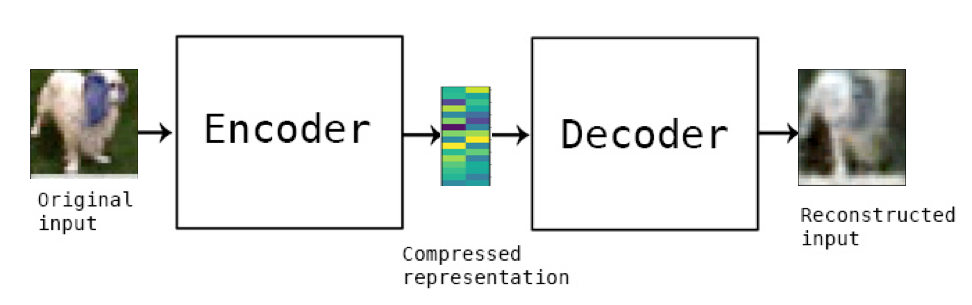
\includegraphics[width=.40\linewidth]{images/transferLearningAE}%
% }\hspace{0.5cm}
% \subfloat[one-class neural networks. \label{sfig:oc-nn-model-architecture}]{%
%   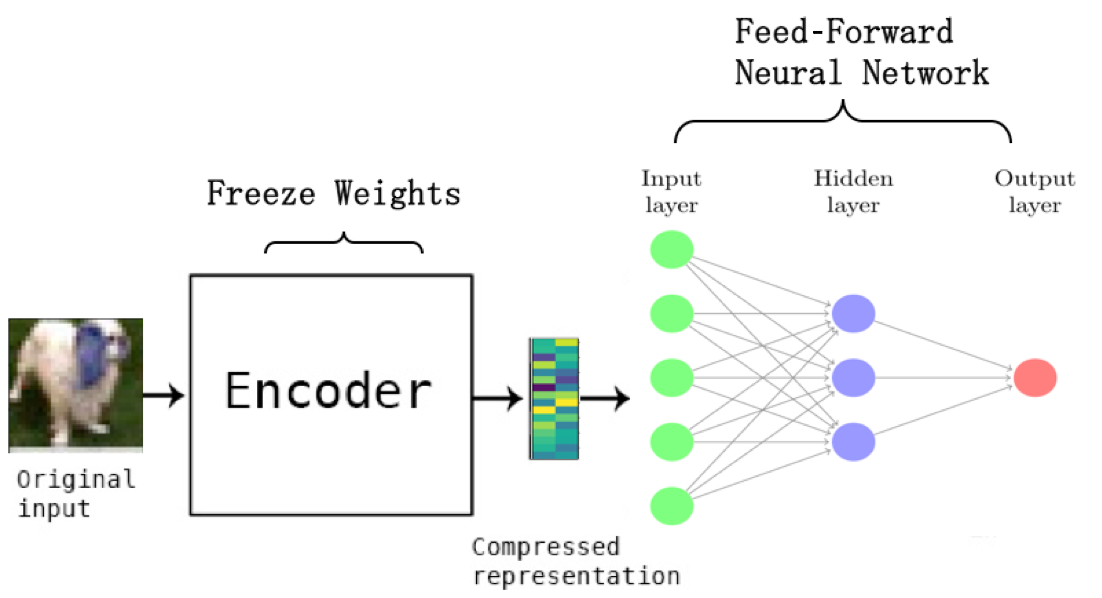
\includegraphics[width=.40\linewidth]{images/oneClassNN_model}%
% }
% \caption{Model architecture of Autoencoder  and the proposed one-class neural networks (OC-NN).}
% \label{fig:model-architecture}
% \end{figure*}
%  End of the Figure

\begin{figure}[!t]
     \begin{subfigure}[b]{1\textwidth}
   \centering
   {\includegraphics[scale=0.50]%{catswithrotatedcats}}
{images/transferLearningAE}}
\caption{Autoencoder.}
        \end{subfigure}%
        \hfill
        \vspace{2mm}
     \begin{subfigure}[b]{1\textwidth}
\centering
   {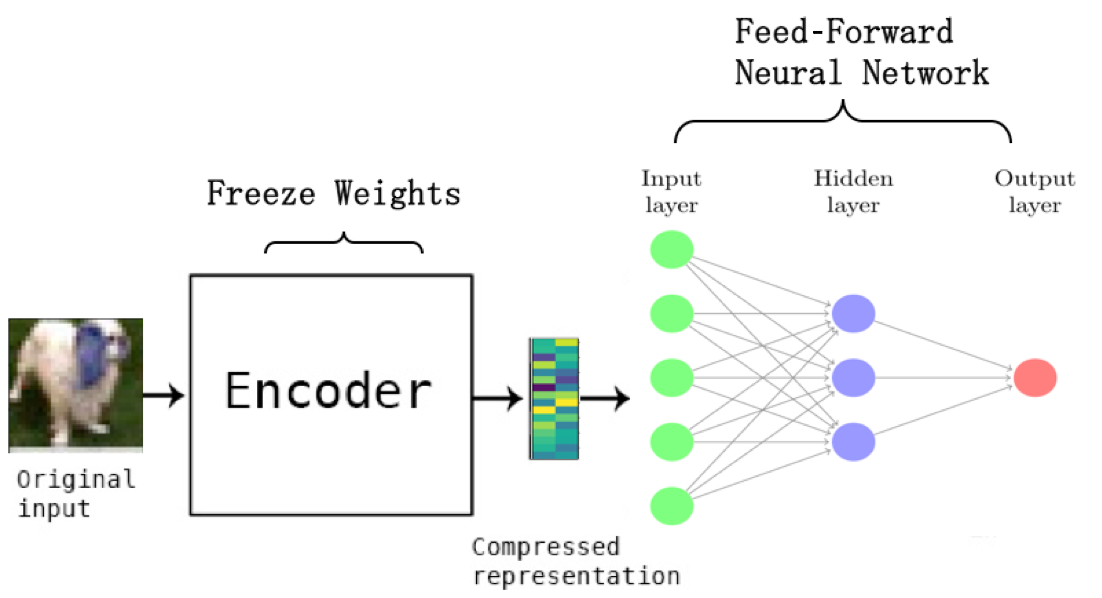
\includegraphics[scale=0.50]{images/oneClassNN_model}}
 \caption{One-class neural networks.}
        \end{subfigure}%
    \caption{
     Model architecture of Autoencoder  and the proposed one-class neural networks (OC-NN).
    }
    \label{fig:model-architecture}
\end{figure}




%Table containing the feed forward network architectures used in experiments
\begin{table}[!t]
    \centering
    \renewcommand{\arraystretch}{1.25}
    \setlength{\tabcolsep}{6pt}
    %\scalebox{0.85}{
    \begin{tabular}{@{}llll@{}}
        \toprule
        \toprule
         Dataset& \#    Input (features) & \# hidden layer( or output) \# optional layer  \\
        \toprule
        {\tt Synthetic }      & 512     & 128   & 1 \\
        {\tt MNIST}           & 32      & 32    & None \\
        {\tt CIFAR$-$10}      & 128     & 32    & None \\
        {\tt GTSRB }          & 128     & 32    & 16 \\
        \bottomrule
    \end{tabular}
    %}
    %\vspace{0.1 cm}
    \caption{Summary of best performing feed-forward network architecture's used in OC-NN model for experiments.}
    \label{tbl:feed-forward-OC-NN}
    \vspace{-\baselineskip}
\end{table}
% end of the table

% \begin{figure}
%     \centering
%     \includegraphics[scale=0.38]{images/s1}
%     \caption{Decision Score Histogram of anomalous vs normal data points, {\tt synthetic} dataset.}
%     \label{fig:synthetic-histogram}
% \end{figure}
































% % The new  experimental setup and results are forthcoming, and that there were technical issues discovered with previously posted results.

% % !TEX root=../main.tex
\section{Experimental Results}
\label{sec:ocnnexperiment-results}

In this section, we present empirical results produced by OC-NN model on synthetic and real data sets. We perform a comprehensive set of experiments to demonstrate that on complex data sets OC-NN performs on par with state-of-the-art methods and outperformed conventional shallow methods in some scenarios.
%%%%% Synthetic Dataset
\subsection{ Synthetic Data}
Single cluster consisting of 190 data points using $\mu=0$ and $\sigma = 2$ are generated as normal points , along with 10 anomalous points drawn from normal distribution with $\mu=0$ and $\sigma = 10$ having  dimension $d=512$. Intuitively, the latter normally distributed points are treated as being anomalous, as the corresponding points have different distribution characteristics to the majority of the training data. Each data point is flattened as a row vector, yielding a 190 $\times$ 512 training matrix and 10 $\times$ 512 testing matrix. We use a simple feed-forward neural network model with one-class neural network  objective as per Equation~\ref{eqn:oc-nn}.\\
%using network parameter settings described in Section~\ref{sec:feed forward oc-nn-model-config}.\\
\textbf{Results}.
From Figure~\ref{fig:synthetic-histogram}, we see that it is a near certainty for all $10$ anomalous points, are accurately identified as outliers with decision scores being negative for anomalies. It is evident that, the OC-NN formulation performs on par with classical OC-SVM in detecting the anomalous data points. In the next sections we apply to image and sequential data and demonstrate its effectiveness.


%% Results for Synthetic dataset
\begin{figure}
    \centering
    \includegraphics[scale=0.38]{images/s1}
    \caption{Decision Score Histogram of anomalous vs normal data points, {\tt synthetic} dataset.}
    \label{fig:synthetic-histogram}
\end{figure}

  % Begin figure
  \begin{figure}[htp]
    % Fixed length
    \centering
    \subcaptionbox{Normal samples.\label{fig3:a}}{\includegraphics[height=8cm,width=1.6in]{images/mnistNormalRCAE}}\hspace{1em}%
    \subcaptionbox{In-class anomalies.\label{fig3:b}}{\includegraphics[height=8cm,width=1.6in]{images/mnistAnomalyRCAE}}
    \caption{MNIST Most normal and in-class anomalous MNIST digits detected by RCAE.}
    \label{fig:mnistRCAEresults}
  \end{figure}
  % End of figure



    % Begin figure
    \begin{figure}[htp]
      % Fixed length
      \centering
      \subcaptionbox{Normal samples.\label{fig3:a}}{\includegraphics[height=8cm,width=1.6in]{images/mnistnormalOCNN}}\hspace{1em}%
      \subcaptionbox{In-class anomalies.\label{fig3:b}}{\includegraphics[height=8cm,width=1.6in]{images/mnistOutlierOCNN}}
      \caption{MNIST Most normal and in-class anomalous MNIST digits detected by OC-NN.}
            \label{fig:mnistOCNNresults}
    \end{figure}
    % End of figure


%%%%% Mnist Dataset
\subsection{ OC-NN on MNIST and CIFAR-10}
\textbf{Setup}
Both MNIST and CIFAR-10  have ten different classes from which we construct one-class classification dataset.  One of the classes is the normal class and
samples from the remaining classes represent anomalies. We use the original training and test splits in our
experiments and only train with training set examples from
the respective normal class. This produces normal instances set of sizes
of n $\approx$ 6000 for MNIST and n $\approx$ 5000 for CIFAR-10 respectively.
Both MNIST and CIFAR-10 test sets have $10000$ samples per class.
The training set comprises of normal instances for each class along with anomalies sampled from
all the other nine classes. The number of anomalies used within training set consists of 1\% normal class for MNIST and  10\% of normal class for CIFAR-10 dataset respectively. We pre-process all images with global contrast normalization using the $L1$
norm and finally rescale to [0, 1] via min-max-scaling.\\
\textbf{Network architectures} For both MNIST and CIFAR-10 datasets, we employ LeNet type
CNNs, wherein each convolutional module consists of a convolutional layer followed by leaky ReLU activations and $2 \times 2$ max-pooling. On MNIST, we use a CNN with two modules, $8\times(5\times5\times1)$-filters followed by $4\times(5\times5\times1)$-filters, and a final dense layer of 32 units. On CIFAR-10,
we use a CNN with three modules, $32 \times (5 \times 5 \times3)$-filters,
$64\times(5\times5\times3)$-filters, and $128\times(5\times5\times3)$-filters, followed
by a final dense layer of $128$ units. We use a batch size of
$200$ and set the weight decay hyperparameter to $ \lambda= 10^{ - 5}$.\\
{\textbf{Results:}}
Results are presented in Table ~\ref{tab:ocnn_results}. RCAE
clearly outperforms both its shallow and deep competitors
on MNIST. On CIFAR-10 the results are convincing but for certain classes the shallow baseline methods outperform the deep models. OC-NN, Soft and One-class Deep SVDD however, shows an overall robust performance. On CIFAR-10 classes such as $AUTOMOBILE$, $BIRD$ and $DEER$ which have less global contrast, as illustrated in Table~\ref{tab:ocnn_results} (indicated in blue color)  OC-NN seems to outperform the shallow methods, Soft and One-class Deep SVDD methods, this is indicative of their future potential on similar data instances.  It is interesting to note that shallow OCSVM/SVDD and KDE perform better than deep methods on two of the ten CIFAR-10 classes. We can see that normal examples of the classes  such as $FROG$ and $TRUCK$ on which OCSVM/SVDD performs best as illustrated in Figure~\ref{fig:ocsvmresults} seem to have strong global structures. For example, TRUCK images are mostly divided horizontally into street and sky, and  $FROG$ have similar colors globally. For these classes,  the performance significantly depends on choice of network architecture. Notably, the One-Class Deep SVDD performs slightly better than its soft-boundary counterpart on both datasets. Figure ~\ref{fig:mnistRCAEresults},  Figure ~\ref{fig:cifar10_rcae_results}  and Figure ~\ref{fig:mnistOCNNresults}, Figure ~\ref{fig:cifar10_ocnn_results} show examples of the most normal and most anomalous in-class samples detected by RCAE and OC-NN for MNIST and CIFAR-10 dataset respectively.


% % Results for Most anomalous and most normal images detected for CIFAR10 dataset
% Figure Begin
\begin{figure}[htp]
    % Fixed length
    \centering
    \subcaptionbox{Normal samples.\label{fig3:a}}{\includegraphics[width=1.6in]{images/cifar10NormalRCAE}}\hspace{1em}%
    \subcaptionbox{In-class anomalies.\label{fig3:b}}{\includegraphics[width=1.6in]{images/cifar10AnomalyRCAE}}
  \caption{CIFAR-10 Most normal and in-class anomalous CIFAR10 digits detected by RCAE. }
  \label{fig:cifar10_rcae_results}
\end{figure}
  % End of figure

% Begin figure
\begin{figure}[htp]
      % Fixed length
      \centering
      \subcaptionbox{Normal samples.\label{fig3:a}}{\includegraphics[width=1.6in]{images/cifar10normalOCNN}}\hspace{1em}%
      \subcaptionbox{In-class anomalies.\label{fig3:b}}{\includegraphics[width=1.6in]{images/cifar10OutlierOCNN}}
    \caption{CIFAR-10 Most normal and in-class anomalous CIFAR10 digits detected by OC-NN. }
    \label{fig:cifar10_ocnn_results}
\end{figure}
% end of figure




% % Results for Most anomalous and most normal images detected for CIFAR10 dataset
% Figure Begin
\begin{figure}[htp]
          % Fixed length
          \centering
          \subcaptionbox{Normal samples.\label{fig3:a}}{\includegraphics[width=1.6in]{images/cifar10normalOCSVM}}\hspace{1em}%
          \subcaptionbox{In-class anomalies.\label{fig3:b}}{\includegraphics[width=1.6in]{images/cifar10OutlierOCSVM}}
       \caption{Most normal (left) and most anomalous (right) in-class
       examples determined by OCSVM-SVDD for in which OCSVM-SVDD performs best.}
        \label{fig:ocsvmresults}
 \end{figure}


\subsection{ Detecting Adversarial attacks on GTSRB stop signs using OC-NN }
\textbf{Setup:}
In many applications (eg. autonomous driving) it is of paramount interest to effectively detect the adversarial samples to ensure safety and security. In this experiment, we
examine  the performance of proposed algorithms on  detecting
adversarial examples. We consider the “stop sign”
class of the German Traffic Sign Recognition Benchmark
(GTSRB) dataset, for which we generate adversarial examples
from randomly drawn stop sign images of the test set
using Boundary Attack~\cite{brendel2017decision}. We create training dataset consists of n = 1150 examples obtained by combining the normal and anomalous samples in both train and test samples. The  number of normal instances n = 1050 stop signs ( 780  from train set +  270 test set ) alongwith  100
adversarial examples are added to obtain training set. We pre-process the
data by removing the 10\% border around each sign, and then resize every image to $32 \times 32$ pixels following the same setup as in ~\cite{pmlrv80ruff18a}. Furthermore, we  apply global contrast normalization using the $L1-norm$ and rescale to the unit interval $[0, 1]$.\\
\textbf{Network architecture} We use a CNN with LeNet architecture having three convolutional modules, $16\times(5\times5\times3)$-filters, $32 \times (5 \times 5 \times 3)$-filters, and $64 \times (5 \times 5 \times 3)$-filters, followed by a final dense layer of 32 units. We train with a smaller batch size of 64, due to the dataset size and set again hyperparamter $\lambda = 10^{ - 6}$.\\
\textbf{Results:}
Results Table ~\ref{tab:gtsrbresults} illustrates the AUC scores obtained. The RCAE outperforms all the other deep models. Figure ~\ref{fig:gtsrbrcaeresults} and Figure ~\ref{fig:gtsrbocnnresults}  shows the most anomalous samples detected by RCAE and OCNN methods respectively, the outliers in this experiment are the images in odd perspectives and the ones that are cropped incorrectly.

\begin{table*}[!t]
   \caption{Average AUCs in \% with StdDevs (over 10 seeds) per method on MNIST and CIFAR-10 dataset.}
   \label{tab:ocnn_results}
   \small % text size of table content
   \centering % center the table
   \scalebox{0.6}{
   \begin{tabular}{lccccccccr} % alignment of each column data
   \toprule[\heavyrulewidth]\toprule[\heavyrulewidth]
   \textsc{\pbox{20cm}{Normal \\ Class}} & \textsc{\pbox{20cm}{OCSVM / \\ SVDD}} & \textsc{KDE} &  \textsc{IF} & \textsc{DCAE} & \textsc{ANOGAN} & \textsc{\pbox{20cm}{SOFT-BOUND \\ DEEP SVDD}} & \textsc{\pbox{20cm}{ONE-CLASS \\ DEEP SVDD}} & \textsc{OC-NN} & \textsc{RCAE} \\
   \midrule
   0 & $96.75\pm0.5$ & $97.1\pm0.0$ & $95.32\pm1.2$  & $99.90\pm0.0$ & $96.6\pm1.3$ & $98.66\pm1.3$     & $97.78\pm0.0$ & $97.60\pm1.7$ &
   $\bf{99.92\pm0.0}$\\
   1 & $99.15\pm0.4$ & $98.9\pm0.0$ & $99.35\pm0.0$  & $99.96\pm2.1$ & $99.2\pm0.6$ & $99.15\pm0.0$     & $99.08\pm0.0$ & $\color[rgb]{0,0,1}99.53\pm0.0$ & $\bf{99.97\pm2.2}$\\
   2 & $79.34\pm2.2$ & $79.0\pm0.0$ & $73.15\pm4.5$  & $96.64\pm1.3$ & $85.0\pm2.9$ & $88.09\pm2.2$     & $88.74\pm1.2$ & $87.32\pm2.1$ & $\bf{98.01\pm1.2}$\\
   3 & $85.88\pm1.3$ & $86.2\pm0.0$ & $81.34\pm2.8$ & $98.42\pm0.0$ &  $88.7\pm2.1$ &  $88.93\pm3.4$     & $88.26\pm3.2$ & $86.52\pm3.9$ & $\bf{99.25\pm0.0}$\\
   4 & $94.18\pm1.5$ & $87.9\pm0.0$ & $87.40\pm2.6$  & $98.72\pm0.0$ & $89.4\pm1.3 $& $93.88\pm2.3$     & $95.24\pm1.4$ & $93.25\pm2.4$ & $\bf{99.23\pm0.0}$\\
   5 & $72.77\pm3.7$ & $73.8\pm0.0$ & $73.96\pm2.9 $ & $97.80\pm1.3$ & $88.3\pm2.9$ & $84.35\pm3.1$     & $83.76\pm3.1$ & $\color[rgb]{0,0,1}86.48\pm3.3$ &$ \bf{99.21\pm0.0}$\\
   6 & $95.14\pm1.1$ & $87.6\pm0.0$ & $88.65\pm0.0$  & $99.74\pm0.0$ & $94.7\pm2.7$ & $97.74\pm0.0$     & $97.99\pm0.0$ & $97.12\pm1.4$ & $\bf{99.81\pm1.1}$\\
   7 & $91.86\pm1.6$ & $91.4\pm0.0$ & $91.44\pm1.8$  & $99.08\pm2.2$ & $93.5\pm1.8$ & $92.60\pm1.2$     & $93.55\pm2.3$ & $93.64\pm2.1$ & $\bf{99.18\pm0.0}$\\
   8 & $88.65\pm1.2$ & $79.2\pm0.0$ & $75.10\pm3.7$  & $96.98\pm0.0$ & $84.9\pm2.1$ & $90.69\pm3.3$     & $90.25\pm3.1$ & $88.54\pm4.7$ & $\bf{98.50\pm2.2}$\\
   9 & $92.53\pm1.9$ & $88.2\pm0.0$ & $87.59\pm1.5$  & $98.04\pm1.3$ & $92.4\pm1.1$ & $94.28\pm2.5$     & $94.12\pm2.4$ & $93.54\pm3.3$ & $\bf{98.98\pm1.3}$\\
   \hline
  \textsc{Aeroplane}    & $60.37\pm1.3$ & $61.2\pm0.0$ & $63.99\pm1.1$  &$71.21\pm1.5$& $67.1\pm2.5$ & $66.15\pm1.1$ & $67.33\pm2.2$ & $60.42\pm1.9$  & $\bf{72.04\pm2.5}$\\
   \textsc{Automobile}  & $63.03\pm1.4$ & $63.0\pm0.0$ & $60.56\pm1.0$  &$63.05\pm2.3$& $54.7\pm3.4 $& $57.64\pm3.2$ & $58.14\pm3.1$ & $\color[rgb]{0,0,1}61.97\pm2.0$  & $\bf{63.08\pm2.1}$\\
   \textsc{Bird}        & $63.47\pm1.0 $& $50.1\pm0.0$ & $64.51\pm1.1$  &$71.50\pm1.1$& $52.9\pm3.0 $& $61.99\pm1.4$ & $61.35\pm1.5$ & $\color[rgb]{0,0,1} {63.66\pm1.4}$ & $\bf{71.67\pm1.3}$\\
   \textsc{Cat}         & $60.25\pm0.9$ & $56.4\pm0.0$ & $56.16\pm2.6$  &$60.57\pm0.0$& $54.5\pm1.9$ & $57.56\pm4.1$ & $55.72\pm1.4$ & $53.57\pm2.1$  & $\bf{60.63\pm1.1}$\\
  \textsc{Deer}         & $69.15\pm0.8$ & $66.2\pm0.0 $& $72.66\pm1.1 $ &$70.85\pm2.2$& $65.1\pm3.2$ & $63.36\pm1.3$ & $63.32\pm1.2$ & $\color[rgb]{0,0,1}67.40\pm1.7 $ & $\bf{72.75\pm3.3}$\\
   \textsc{Dog}         & $66.24\pm1.5$ & $62.4\pm0.0$ & $61.46\pm2.7 $ &$62.74\pm2.1$& $60.3\pm2.6$ & $58.58\pm1.2$ & $58.68\pm1.4$ & $56.11\pm2.1$  & $\bf{63.96\pm3.3}$\\
   \textsc{Frog}        & $\bf{71.57\pm1.5}$ & ${71.3\pm0.0}$ & $68.06\pm2.1 $ &$65.17\pm4.1$& $58.5\pm1.4 $& $63.93\pm3.1 $& $64.45\pm2.1$ & $63.31\pm3.0$  & ${64.88\pm4.2}$\\
   \textsc{Horse}       & $63.38\pm0.8 $& $62.6\pm0.0$ & $63.04\pm1.5$  &$61.11\pm1.4$& $62.5\pm0.8$ & $60.20\pm2.2$ & $59.80\pm2.6$ & $60.09\pm2.7$  &
   $\bf{63.64\pm0.0}$\\
  \textsc{Ship}         & $60.44\pm1.1$ & ${65.1\pm0.0}$ & $68.01\pm1.3$  &$74.18\pm1.2$& $74.68\pm4.1$ & $70.21\pm1.1$ & $67.44\pm2.2$ & $64.67\pm1.6$  & $\bf{74.72\pm1.1}$\\
  \textsc{Truck}        & $\bf{75.81\pm0.8}$ & ${74.0\pm0.0}$ & $72.83\pm1.1$  &$71.36\pm4.3$& $66.5\pm2.8 $& $72.91\pm3.3$ & $68.03\pm3.2$ &$ 60.32\pm4.9 $ & ${74.47\pm1.5}$\\
   \bottomrule[\heavyrulewidth]
   \end{tabular}}
\end{table*}
% end of the table

% begin of table
\begin{table}[ht]
\caption{Average AUCs in \% with StdDevs (over 10 seeds) per
method on GTSRB stop signs with adversarial attacks.} % title of Table
\centering % used for centering table
\scalebox{0.7}{
\begin{tabular}{l l } % centered columns (4 columns)
\hline\hline %inserts double horizontal lines
\bf{\textsc{Method}} & \bf{\textsc{AUC}}\\ [0.5ex] % inserts table
%heading
\hline % inserts single horizontal line
OC-SVM/SVDD & $52.5 \pm 1.3$ \\ % inserting body of the table
KDE & $51.5 \pm 1.6$ \\
IF & $53.37\pm 2.9$ \\
AnoGAN & - \\
DCAE & $79.1\pm3.0$ \\
SOFT-BOUND. DEEP SVDD & $67.53\pm4.7$ \\
ONE-CLASS. DEEP SVDD & $67.08\pm4.7$ \\
OC-NN & $63.53\pm2.5$ \\
\bf{\bf{RCAE $\lambda =0$}} &\bf{$87.45\pm3.1$} \\
\bf{RCAE} & {$\bf{87.39 \pm 2.7}$} \\ [1ex] % [1ex] adds vertical space
\hline %inserts single line
\end{tabular}}
\label{tab:gtsrbresults}
\end{table}
% end of table



% Begin figure
\begin{figure}[htp]
      % Fixed length
      \centering
      \subcaptionbox{Top 50 Normal.\label{fig3:a}}{\includegraphics[width=1.6in,height=1.6in]{images/most_normalGtsrb}}\hspace{1em}%
      \subcaptionbox{Top 50 anomalies.\label{fig3:b}}{\includegraphics[width=1.6in,height=1.6in]{images/most_anomalousGtsrb}}
      \caption{Most normal and anomalous stop signs detected by RCAE. Adversarial examples are highlighted in green, Normal samples are highlighted in blue}
      \label{fig:gtsrbrcaeresults}
   \end{figure}
% end of figure


% Begin figure
\begin{figure}[htp]
      % Fixed length
      \centering
      \subcaptionbox{Top 50 Normal.\label{fig3:a}}{\includegraphics[width=1.6in,height=1.6in]{images/most_normalGtsrbocnn}}\hspace{1em}%
      \subcaptionbox{Top 50 anomalies.\label{fig3:b}}{\includegraphics[width=1.6in,height=1.6in]{images/most_anomalousGtsrbocnn}}
      \caption{Most normal and anomalous stop signs detected by OC-NN.  Adversarial examples are highlighted in green, Normal samples are highlighted in blue}
      \label{fig:gtsrbocnnresults}
      \end{figure}
% end of figure



% \section{Conclusion}
% \label{sec:conclusion}
% % !TEX root=../main.tex
In this paper, we have proposed a one-class neural network (OC-NN) approach for anomaly detection.
OC-NN uses a one-class SVM (OC-SVM) like loss function to train a neural network.
The advantage of OC-NN is that the features of the hidden layers are constructed for the specific
task of anomaly detection. This approach is substantially different from recently proposed
hybrid approaches which use deep learning features as input into an anomaly detector.  Feature
extraction in hybrid approaches is generic and not aware of the anomaly detection task. To learn
the parameters of the OC-NN network we have proposed a novel alternating minimization approach and
have shown that the optimization of a subproblem in OC-NN is equivalent to a quantile selection
% problem. Experiments on complex image and sequential data sets demonstrates that OC-NN is
% highly accurate. For future work, we would like to build and deploy an end to end system for anomaly
% detection based on OC-NN.






%% Include bibliography
% \bibliographystyle{unsrt}
\bibliographystyle{unsrtnat}
\bibliography{main}


\end{document}
